
{\chapter{Exploring the single-cell RNAseq analysis landscape in timeseries patient derived xenografts}

}
 \label{ch:Chapter5}
 \section{Motivation}

In spite of advanced technologies and treatment, triple negative breast cancer still facing the problems of tumor recurrence and drug resistance.
For any given difference between the types of drug resistance, for example, the expression of a particular gene, it is assumed that differences arise deterministically or probabilistically in the configuration of transcription factors regulating the genes in the tumors. Cancer cells in distinct cell states often exhibit important differences in functional properties depending on which genes are turned on and off resulting in sensitive or resistant phenotype.

The most challenging analysis is to differentiate whether the change in gene expression leading to change in cellular state is stochastic \cite{raj2008nature} and random or its deterministic to produce the same output under similar environment.
Previously it is shown that unique cells within a population can exhibit fluctuations in expression of a group of genes, that could predict distinct phenotypes \cite{shaffer2019memory}.

Although many studies have analyzed CNV and differential gene expression of distinct oncogenes and tumor suppressor genes in various cancers, \cite{kuzyk2015mycn, budczies2016pan, kwak2015fibroblast} but there has been no precise study about the relationship between CNV and differential gene expression across a multiple tumor samples. It is unclear to what extent the expression level is affected by CNV. Because of difficulty to analyse longitudinal patient's samples for single cell gene expression and lack of multiple longitudinal pre-clinical breast cancer models, these questions remains unexplored and how they relate to triple negative breast cancer heterogeneity, is limited.

Here, we aimed to systematically investigate the specific relationship between copy number change and differential gene expression across timeseries TNBC PDX for which we have clonal copy number proportions already known from chapter 4. We set to explore 3 timeseries breast cancer patient derived xenografts (PDX) that were serially challenged for around 4-5 cycles with the drug until they started showing resistant behaviour. The aim is to measure the magnitude of fluctuations in gene expression from sensitive to resistant phenotype.
This study may help us better understand the correlation between CNV and differential gene expression and provide new insights into the mechanism of development and progression of cancer with potential biomarkers in triple negative breast cancer.

 \section{Synopsis}
 %From the previous chapter, we know that the population changes with the tumor growth from one passage to another, with and without the drugs. We see the shifts in the clones and some clones get selected and others disappear.
In this chapter, to explore the cellular compositions and breast cancer heterogeneity under diverse conditions, we performed scRNAseq analysis on the same 3 patient derived xenograft timeseries used as substrates in chapter 4. We acquired transcriptional signatures of 171,560 individual cells. Two libraries from CX-5461 treated samples were excluded from analysis as they didn't pass our QC threshold. Total of 145,858 individual cells were taken into further transcriptome analysis, including  52,256 cells from untreated tumors, 40,754 cells from cisplatin treated tumors, 31,269 cells from cisplatin drug holiday tumors, 8,558 cells from CX-5461 treated tumors and 13,021 cells from CX-5461 drug holiday tumors. The detail after filtering is summarized in  \textbf{\autoref{tab:nofcellsRNA}}.

First, we summarized the clonal identities from chapter 4 into sensitive and resistant and  assumed that the clones that show fitness advantage under drug selection, at DLP+ level, are resistant because they were high abundance clones (tumor growth inhibition was low in those tumors), whereas the clones that are having high fitness coefficient in the absence of drug are sensitive because they could not survive under drug pressure but showed fitness advantage over others in the absence of drug (\textbf{\autoref{tab:Listofresistantandsensitiveclones}}).
 

To pursue our analysis at single cell RNA level, we encompassed on three main queries; (i) how to explain the data processing from our experimental design (ii) how much of the differentially expressed genes in resistant vs sensitive clones are \textit{in cis} or \textit{in trans} regulated and (iii) explore the change of expression overtime.  

\subsection{Data processing and clonal assignments}
 From the data processing metrics, we found that batch effects in samples were partially removed by SCTransform normalization method \cite{hafemeister2019normalization} as well as \texttt{edgeR} \cite{robinson2010edger} for differential gene expression analysis.
Next, by using clonealign \cite{campbell2019clonealign}, we were able to assign single cell RNAseq to clones and observed similar clonal proportion from RNA seq what we concluded in the DLP+ in chapter 4 as expected. Finally, for this section,  
we applied dimentionality reduction embeddings of the cells and revealed that the clones appear to be clustering together with minor exceptions. 
%----------------------------------
% Table generated by Excel2LaTeX from sheet 'Sheet1'
 \begin{table}[htbp]
   
   \centering
   \caption{List of resistant and sensitive clones across TNBC PDX}
     \begin{tabular}{|l|l|l|}
      \hline
     TNBC PDX & Resistant clone & Sensitive clone \\
     \hline
     TNBC-SA609  & Clone A & Clone H \\
     TNBC-SA1035 & Clone H & Clone E \\
     TNBC-SA535-Cisplatin Rx & Clone S\_T & Clone J \\
     TNBC-SA535-CX-5461 Rx & Clone U & Clone J \\    \hline
     \end{tabular}%
   \label{tab:Listofresistantandsensitiveclones}%
   
 \end{table}%
 
%----------------------------------------------------------------

\subsection{Proportions of \textit{in cis} and \textit{in trans} genes in differentially expressed genes} 
In next section, we asked as to how much of the expression is accounted by the change in copy number and what proportion is independent. The global proportions of \textit{in cis} and \textit{in trans} in resistant versus sensitive clones were measured. Then, we looked for the magnitude of difference of upregulated or down regulated genes by calculating differential expression of resistant and sensitive clones through volcano plots analysis. Lastly, we explored which pathways and individual genes are involved in resistant and sensitive clones across all timeseries PDX models. We found few intersecting pathways that seems to be upregulated in all timeseries and some with 2-3

\subsection{Change of expression over time with or without drug exposure}
Lastly, we identified some genes that were increasing or decreasing under continuous drug pressure in our datasets. We were able to identify certain common genes that are showing trends under the drug in all TNBC timeseries PDX that could be further investigated as potential biomarkers of disease progression and tumor response.


%-----------------------------------------------------------------
\begin{figure}
\centering
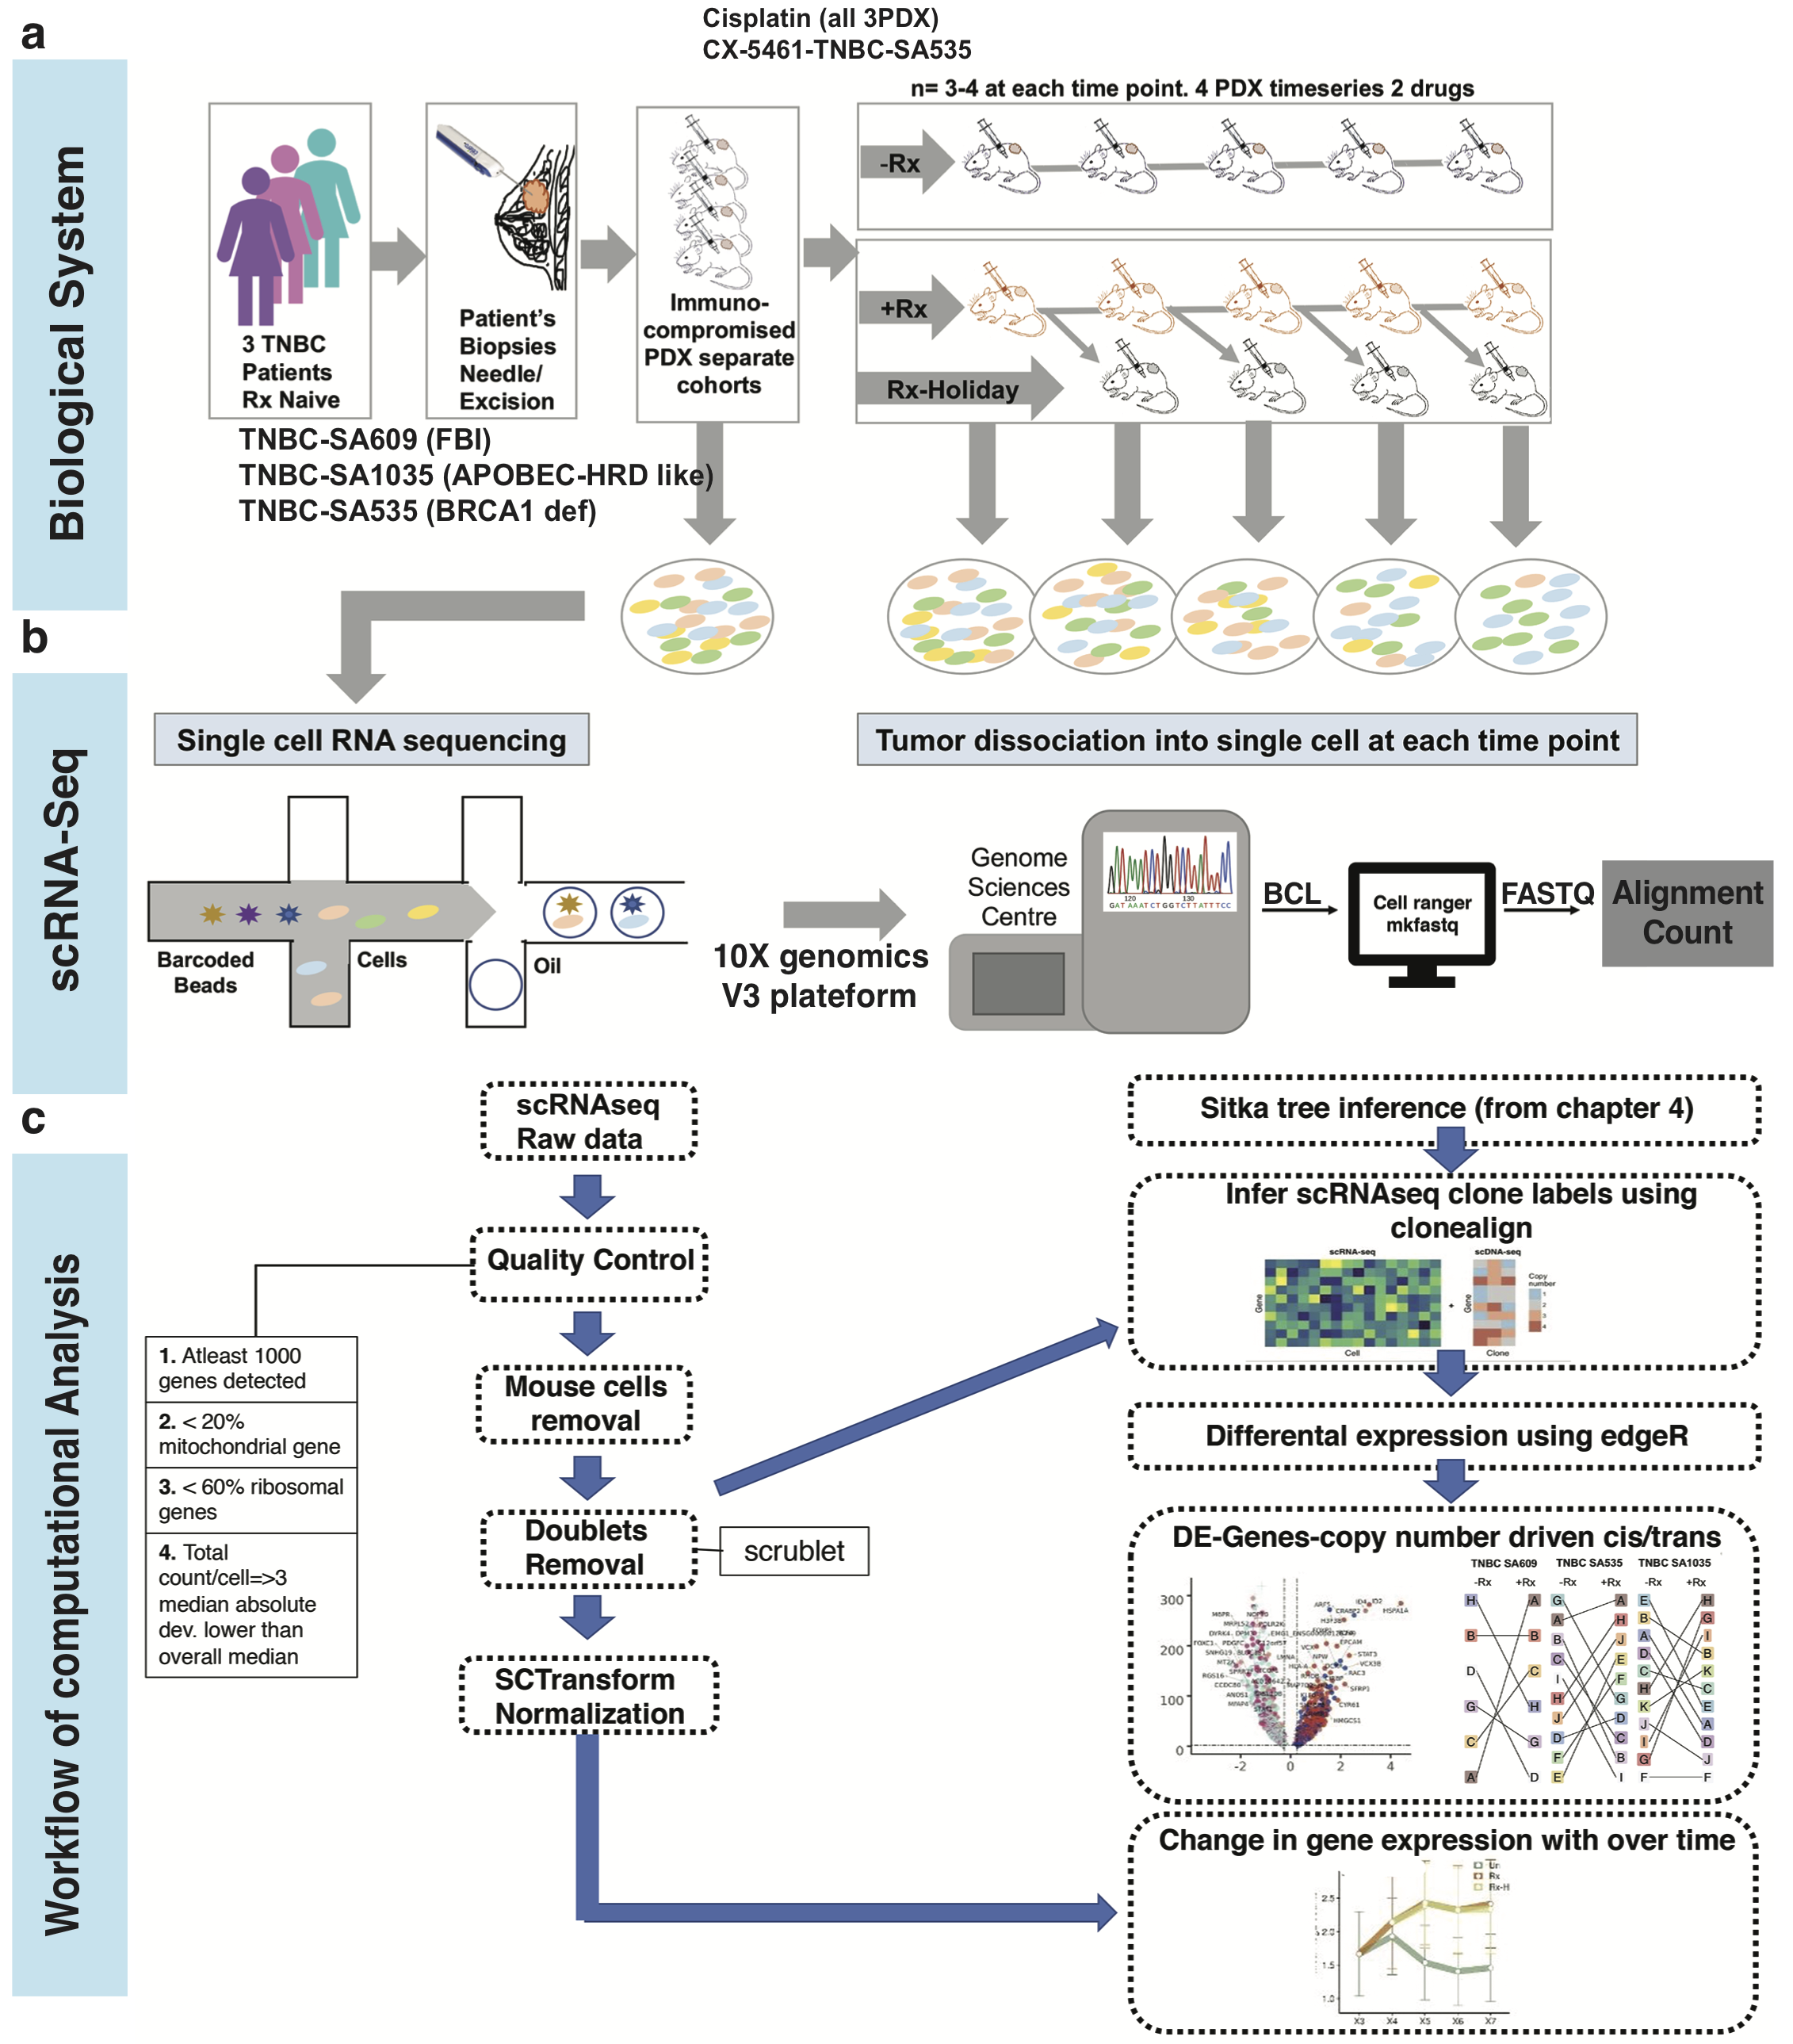
\includegraphics[width=\textwidth]{Figures/chap5/RNAworkflow.png}
	
\caption[Schematics of experimental design and analysis workflow]
	{\small
	\textbf{Schematics of data generation and analysis workflow.}
	   \textbf{(a)} Overview of the experimental design same series as of chapter 4.
	    \textbf{(b)} Single cells RNA library prep. and sequencing.
	    \textbf{(c)} Computational workflow analysis used in this chapter.
	}
	\label{fig:chap5RNAworkflow}
\end{figure}
%----------------------------------------------------------------


\section{Results}
 
 \subsection{Longitudinal single-cell RNA sequencing of patient-derived xenografts reveals complexity of data processing}
  
\subsubsection{Sample collection and workflow of data generation and analysis from triple negative breast cancer timeseries PDX}
To understand resistance at the single cell RNA level, we selected 4  patient-derived xenograft timeseries that were developed by transplanting patient's tumor biopsies in immunodeficient mice as described in chapter 3 (\textbf{\autoref{fig:chap5RNAworkflow} a}). 
Briefly, 3 triple negative breast cancer xenografts (TNBC-SA609, TNBC-SA1035,TNBC-SA535) were serially challenged for 4-5 cycles of (cisplatin) platinum compound until they started showing resistance.
Similar to aforementioned experiments for chapter 4, we collected exactly same tumors to digest and generate single cell RNA libraries using Chromium 10X genomics (chemistry V3) Single Cell 3' Reagent Chemistry kit standard protocol. Libraries were then sequenced on an Illumina Nextseq500/550 (\textbf{\autoref{fig:chap5RNAworkflow} b}). 

The sequenced raw data was passed through the bioinformatic analysis pipeline for downstream exploration of single cell gene expression in all timeseries \textbf{\autoref{fig:chap5RNAworkflow} c}. 
From raw data, cell features and quality output metrics were used to filter cells, remove low quality cells and keep only cells that pass the threshold of quality control. 
We use Scater package to apply quality control filters. Cell is considered as of good quality if (i) at least 1000 genes detected, (ii) less than 20\% of counts (UMIs) mapping to genes from the mitochondrial genome (``mitochondrial genes''), (iii) fewer than 60\% of counts (UMIs) mapping to ribosomal genes, and (iv) the total counts (UMIs) per cell was at most 3 median absolute deviations lower than the overall median. Cells not matching all criteria were filtered using the calculate \ac{QC} Metrics and Outlier functions in the scater package \cite{mccarthy2017scater}.

\texttt{SCTransform} \cite{hafemeister2019normalization} was used as the normalization method for input for (i) \ac{UMAP} embeddings, (ii) genes variations with drug, density (cloud) plots (iii) line plots to show the gene expression overtime. However, clonal assignments from \texttt{sitka} tree inference from chapter 4 was used to run clonealign \cite{campbell2019clonealign} for \ac{scRNAseq} clone labels. Furthermore, downstream analysis for differential expression of genes, between resistant and sensitive clones, used \texttt{edgeR} \cite{robinson2010edger} for differential expression, volcano plots, Manhattan plots to match genome position to change in expression and cancer related pathways analysis (\textbf{\autoref{fig:chap5RNAworkflow} c}).


\subsubsection{Summarization of number of cells and overall read counts of the data}
Tumors from each time points of TNBC-SA609, TNBC-SA1035 and TNBC-SA535 (cisplatin, CX-5461) were collected and enzymatically digested with collagenase/hyaluronidase, for single cell RNA sequencing as DLP+ (\textbf{\autoref{fig:RNAsampletree}}).
Summary of total number of cells sequenced for each library is enlisted in \textbf{\autoref{tab:nofcellsRNA}}. 

The quality metrics for filtered cells used in data analysis are shown in 
\textbf{\autoref{fig:Diagnosticplotsreadcounts}}. 
After filtering cells that have total features by counts greater than 1500 are considered and included in analysis. Interestingly, the data in 4 TNBC-PDX timeseries showed total features by counts or number of counts as greater than 3000.
Only 2 libraries in TNBC-SA1035 (X5-UT-CHIP0071 and X5-UU-CHIP0076) had a little low quality cells than other libraries (~2500 total features by counts) but acceptable and good enough to use. Other exceptions were TNBC-SA535-CX-5461 treated at time points X7 and X9 with low quality, that was excluded from the downstream analysis. 

%----------------------------------------------------------------


\begin{figure}
\centering
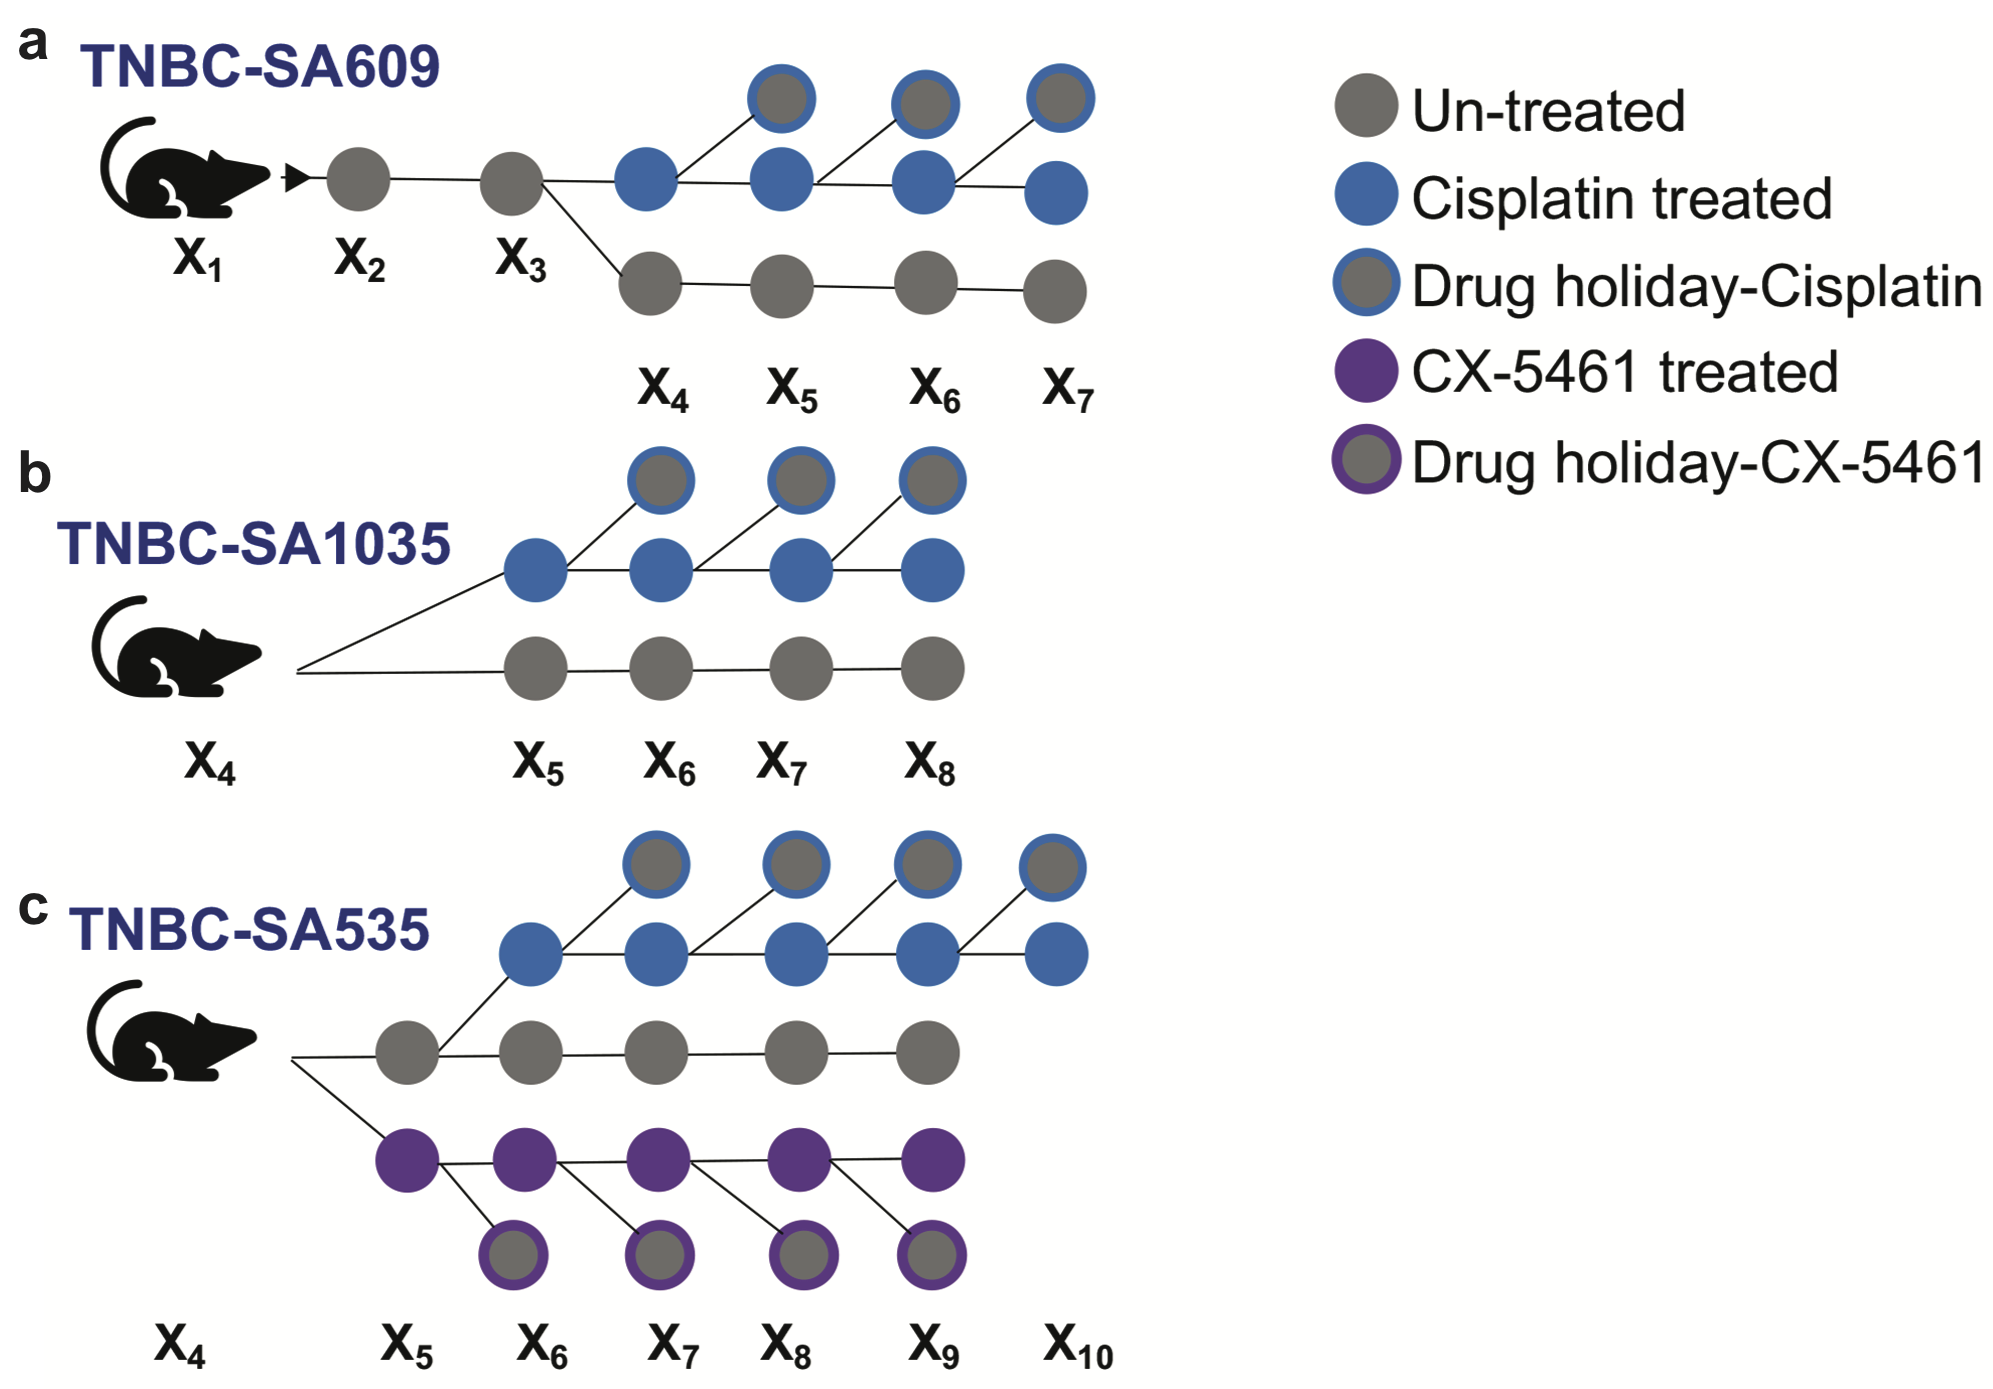
\includegraphics[width=\textwidth]{Figures/chap5/SchematicsforRNAsampling.png}
	
\caption[SchematicsforRNAsampling]
	{\small
	\textbf{Schematics exact tumors used for RNA sampling.}
	   \textbf{(a)} Overview of the experimental design same series as of chapter 4.
	    \textbf{(b)} Single cells RNA library prep. and sequencing.
	    \textbf{(c)} Computational workflow analysis used in this chapter.
	}
	\label{fig:RNAsampletree}
\end{figure}


%----------------------------------------------------------------
\begin{table}[htbp]
 \centering
  \caption{Number of cells sequenced for transcriptome analysis}
{
\begin{tabular}{|l|l|l|}
\hline
Sample labels     & No. of cells sequenced for scRNA & Filtered \\
\hline
Total cells          & 145,858                          & 63,183\\
Untreated         & 52,256                           & 21,510    \\
Cisplatin-Rx      & 40,754                           & 19,095    \\
Cisplatin-holiday & 31,269                           & 15,158    \\
CX-5461-Rx        & 8,558                            & 4,047     \\
CX-5461-holiday   & 13,021                           & 3,373  \\  
\hline
\end{tabular}%
\label{tab:nofcellsRNA}
}
\end{table}


%---------------------------------------------------------------

\begin{figure}
\centering
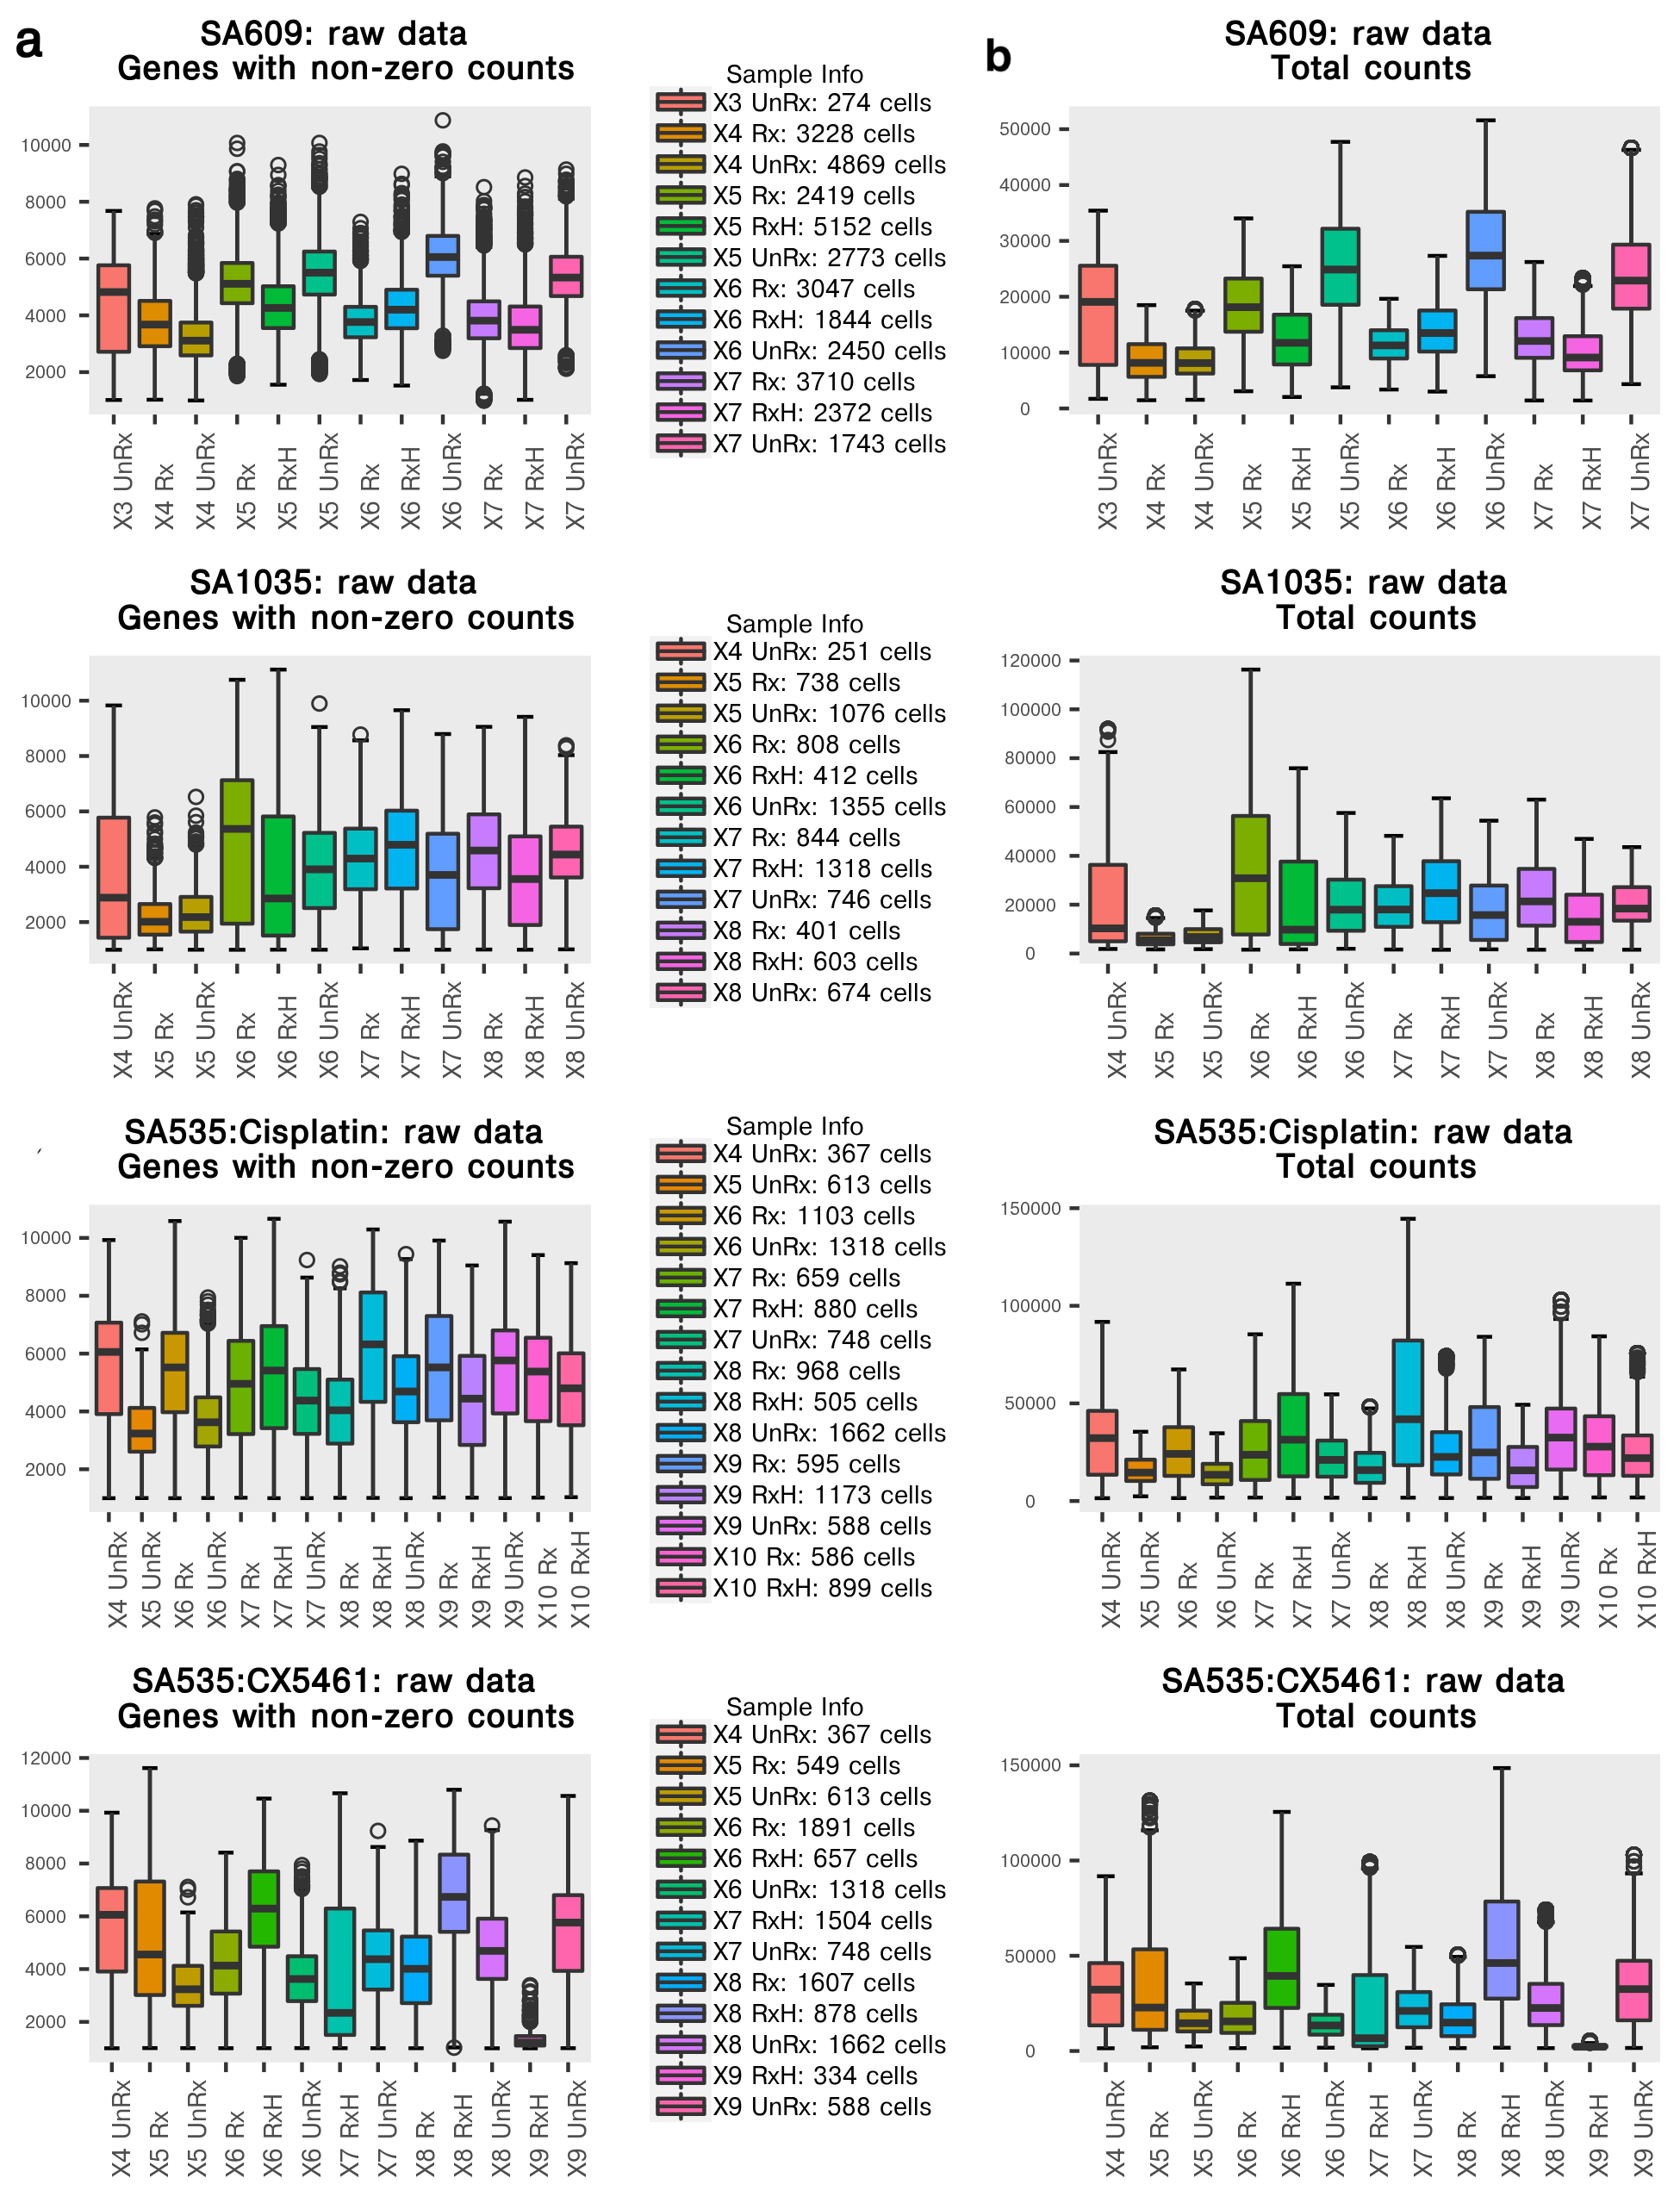
\includegraphics[width=\textwidth]{Figures/chap5/Diagnosticplotsreadcounts.png}
	
\caption[Summary of overall read counts and features of the raw data presented.]
	{\small
	\textbf{Summary of overall read count of the data presented.}
	   \textbf{(a)} Cell-level metric of ``total features by counts'' for all batches of experiments.y-axis denotes total features by counts: the number of genes for each cell that have counts gene expression value above 0. x-axis denotes different batches of experiments, C is ``CHIP0'', same chip number is same batch. x-axis also contain passage info, and treatment status
	    \textbf{(b)} Cell level metric ``total counts'' for all batches of experiments.
	   
	}
	\label{fig:Diagnosticplotsreadcounts}
\end{figure}

%-----------------------------------------------------------

\begin{figure}
\centering
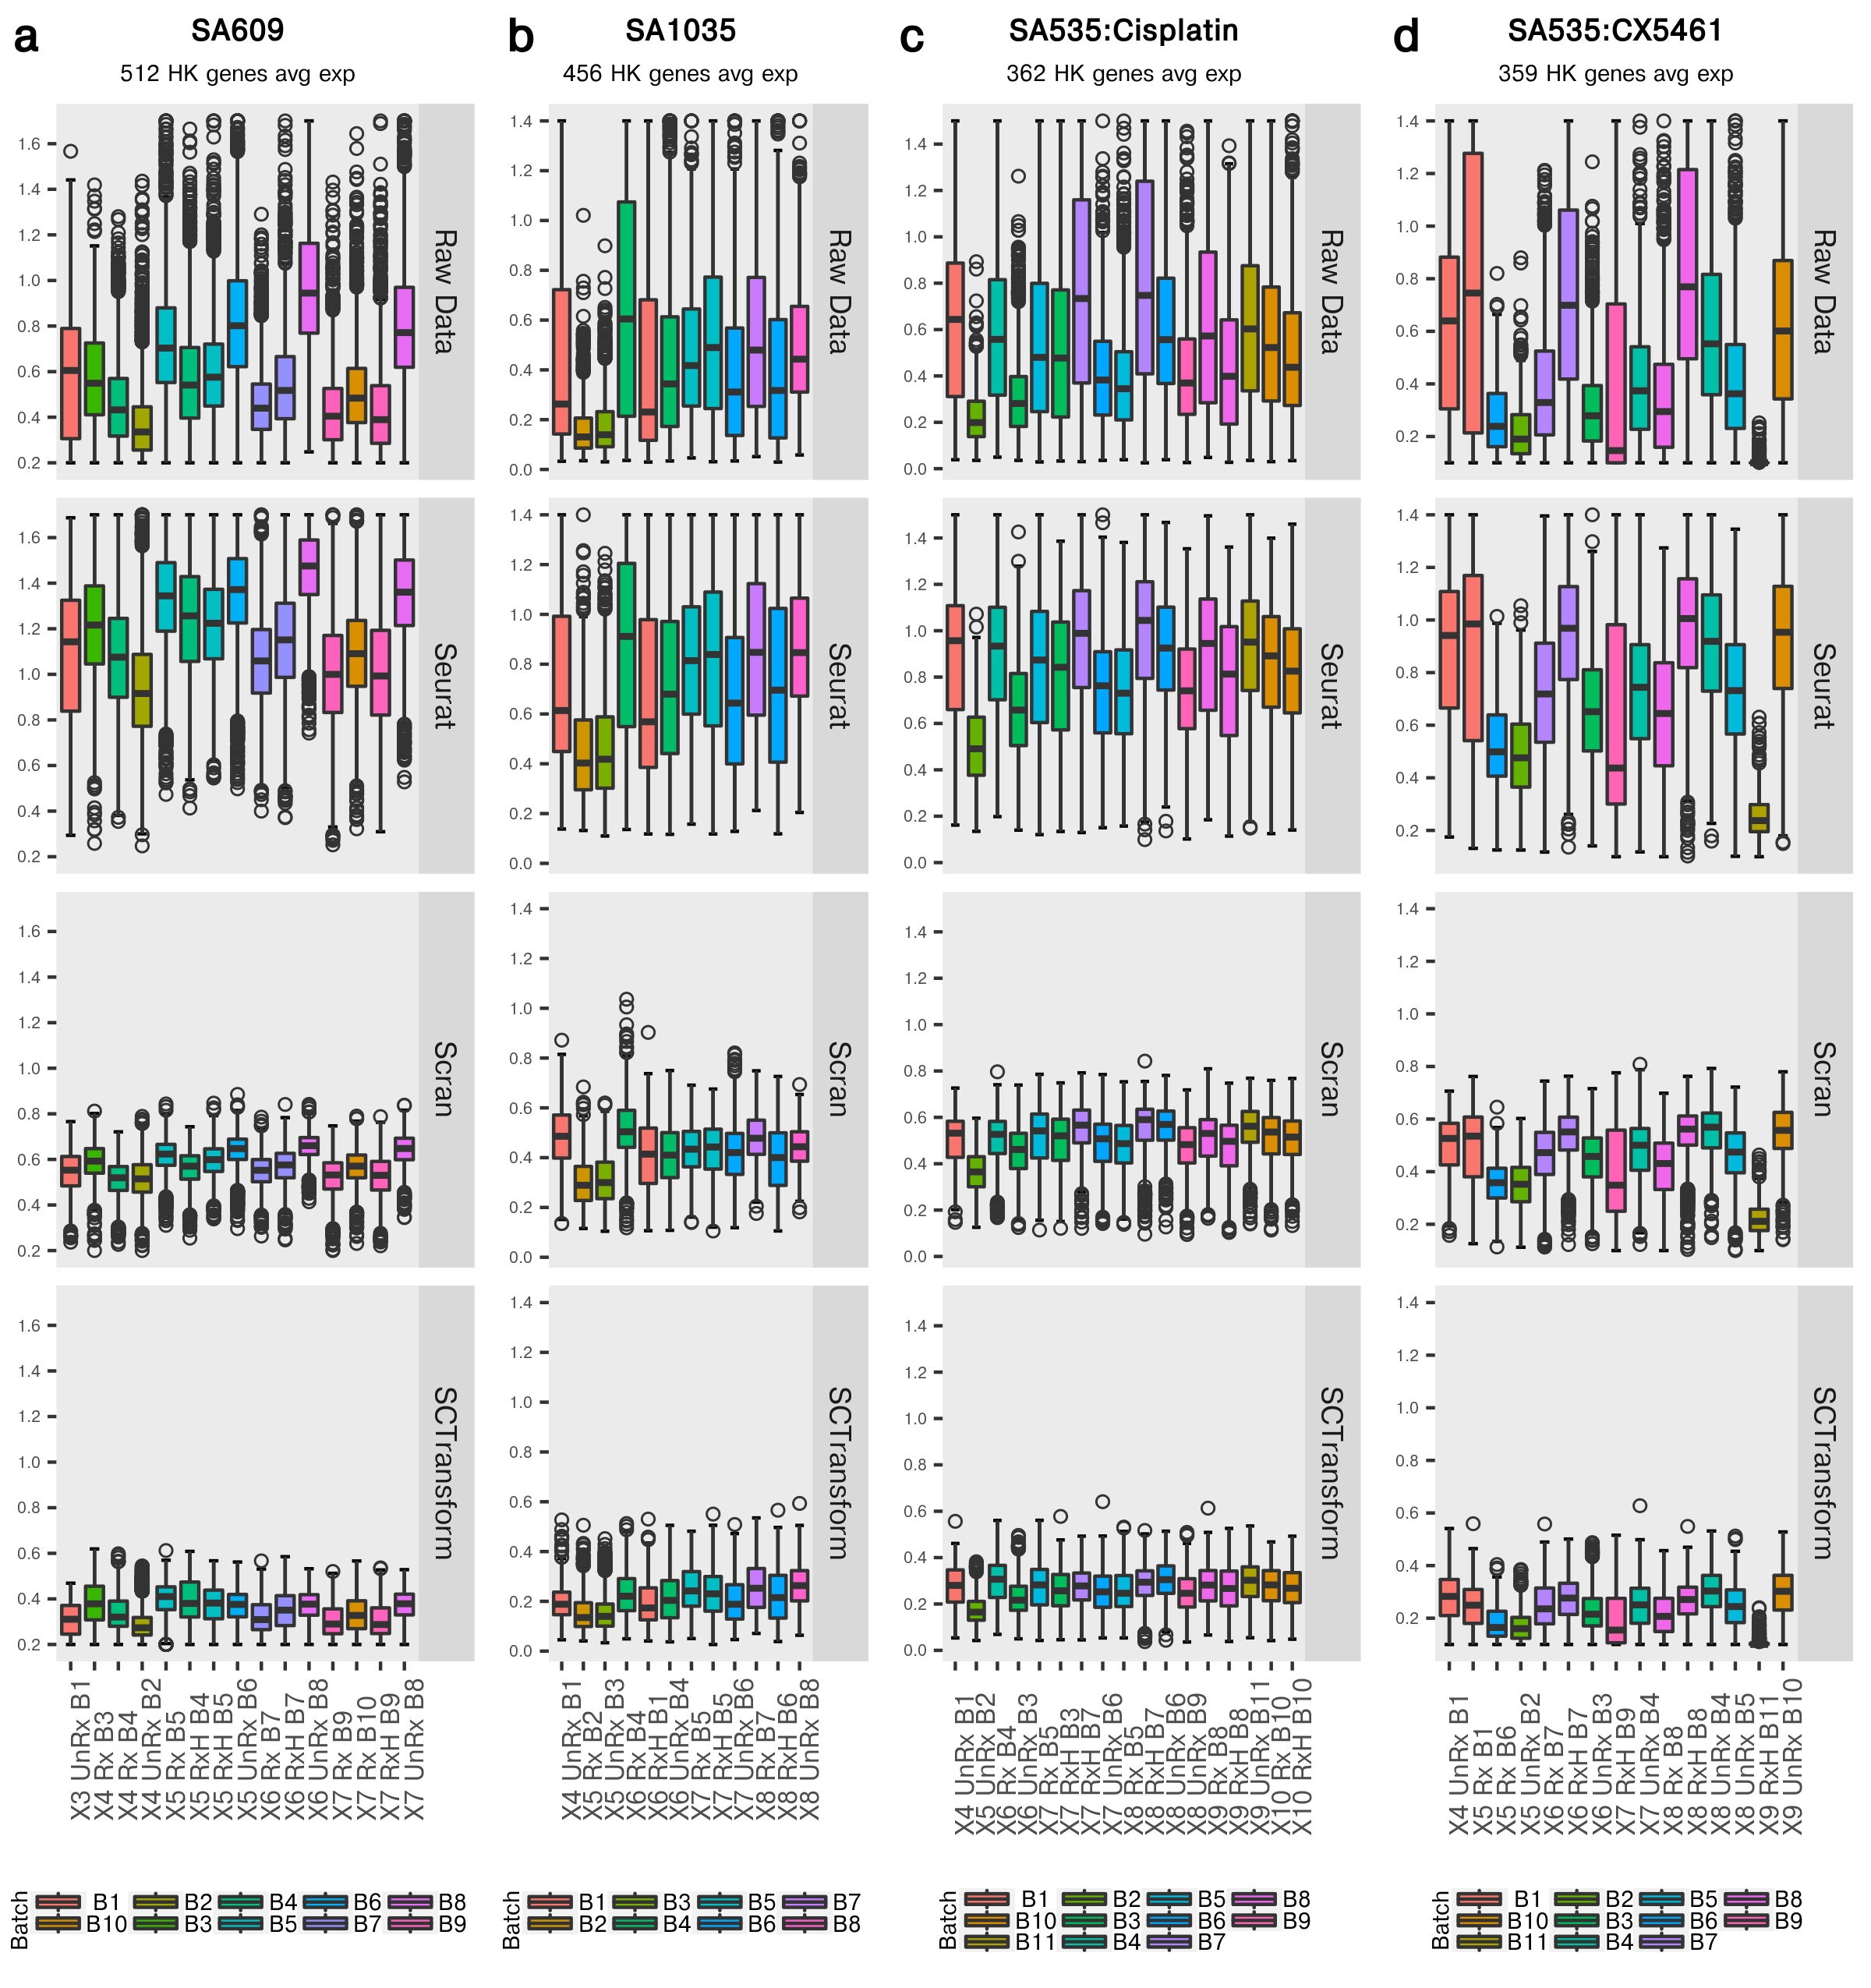
\includegraphics[width=\textwidth]{Figures/chap5/Comparisonofbatcheffects.png}
	
\caption[Summary of overall read count of the data presented.]
	{\small
	\textbf{Evaluation of batch effects in TNBC PDX timeseries data.}
	  House keeping genes were selected from \cite{lin2019evaluating} and mean expression calculated in all timeseries of TNBC PDX. Horizontal axis shows sample IDs from each of that time series and vertical axis shows mean gene expression.
	   \textbf{(a)} Raw data with no normalization showing mean expression of house keeping genes in all 4 treated and untreated TNBC PDX timeseries. 
	    \textbf{(b)} Two times applying scran on data (Twice scran) normalization  in all 4 treated untreated TNBC PDX timeseries.
	    \textbf{(c)} Suerat (normalization) on  all 4 treated and untreated TNBC PDX timeseries.
	    \textbf{(d)} SCTransform (normalization) on  all 4 treated and  untreated TNBC PDX timeseries
	}
	\label{fig:Comparisonofbatcheffects}
\end{figure}
%-----------------------------------------------------------------

\begin{figure}
\centering
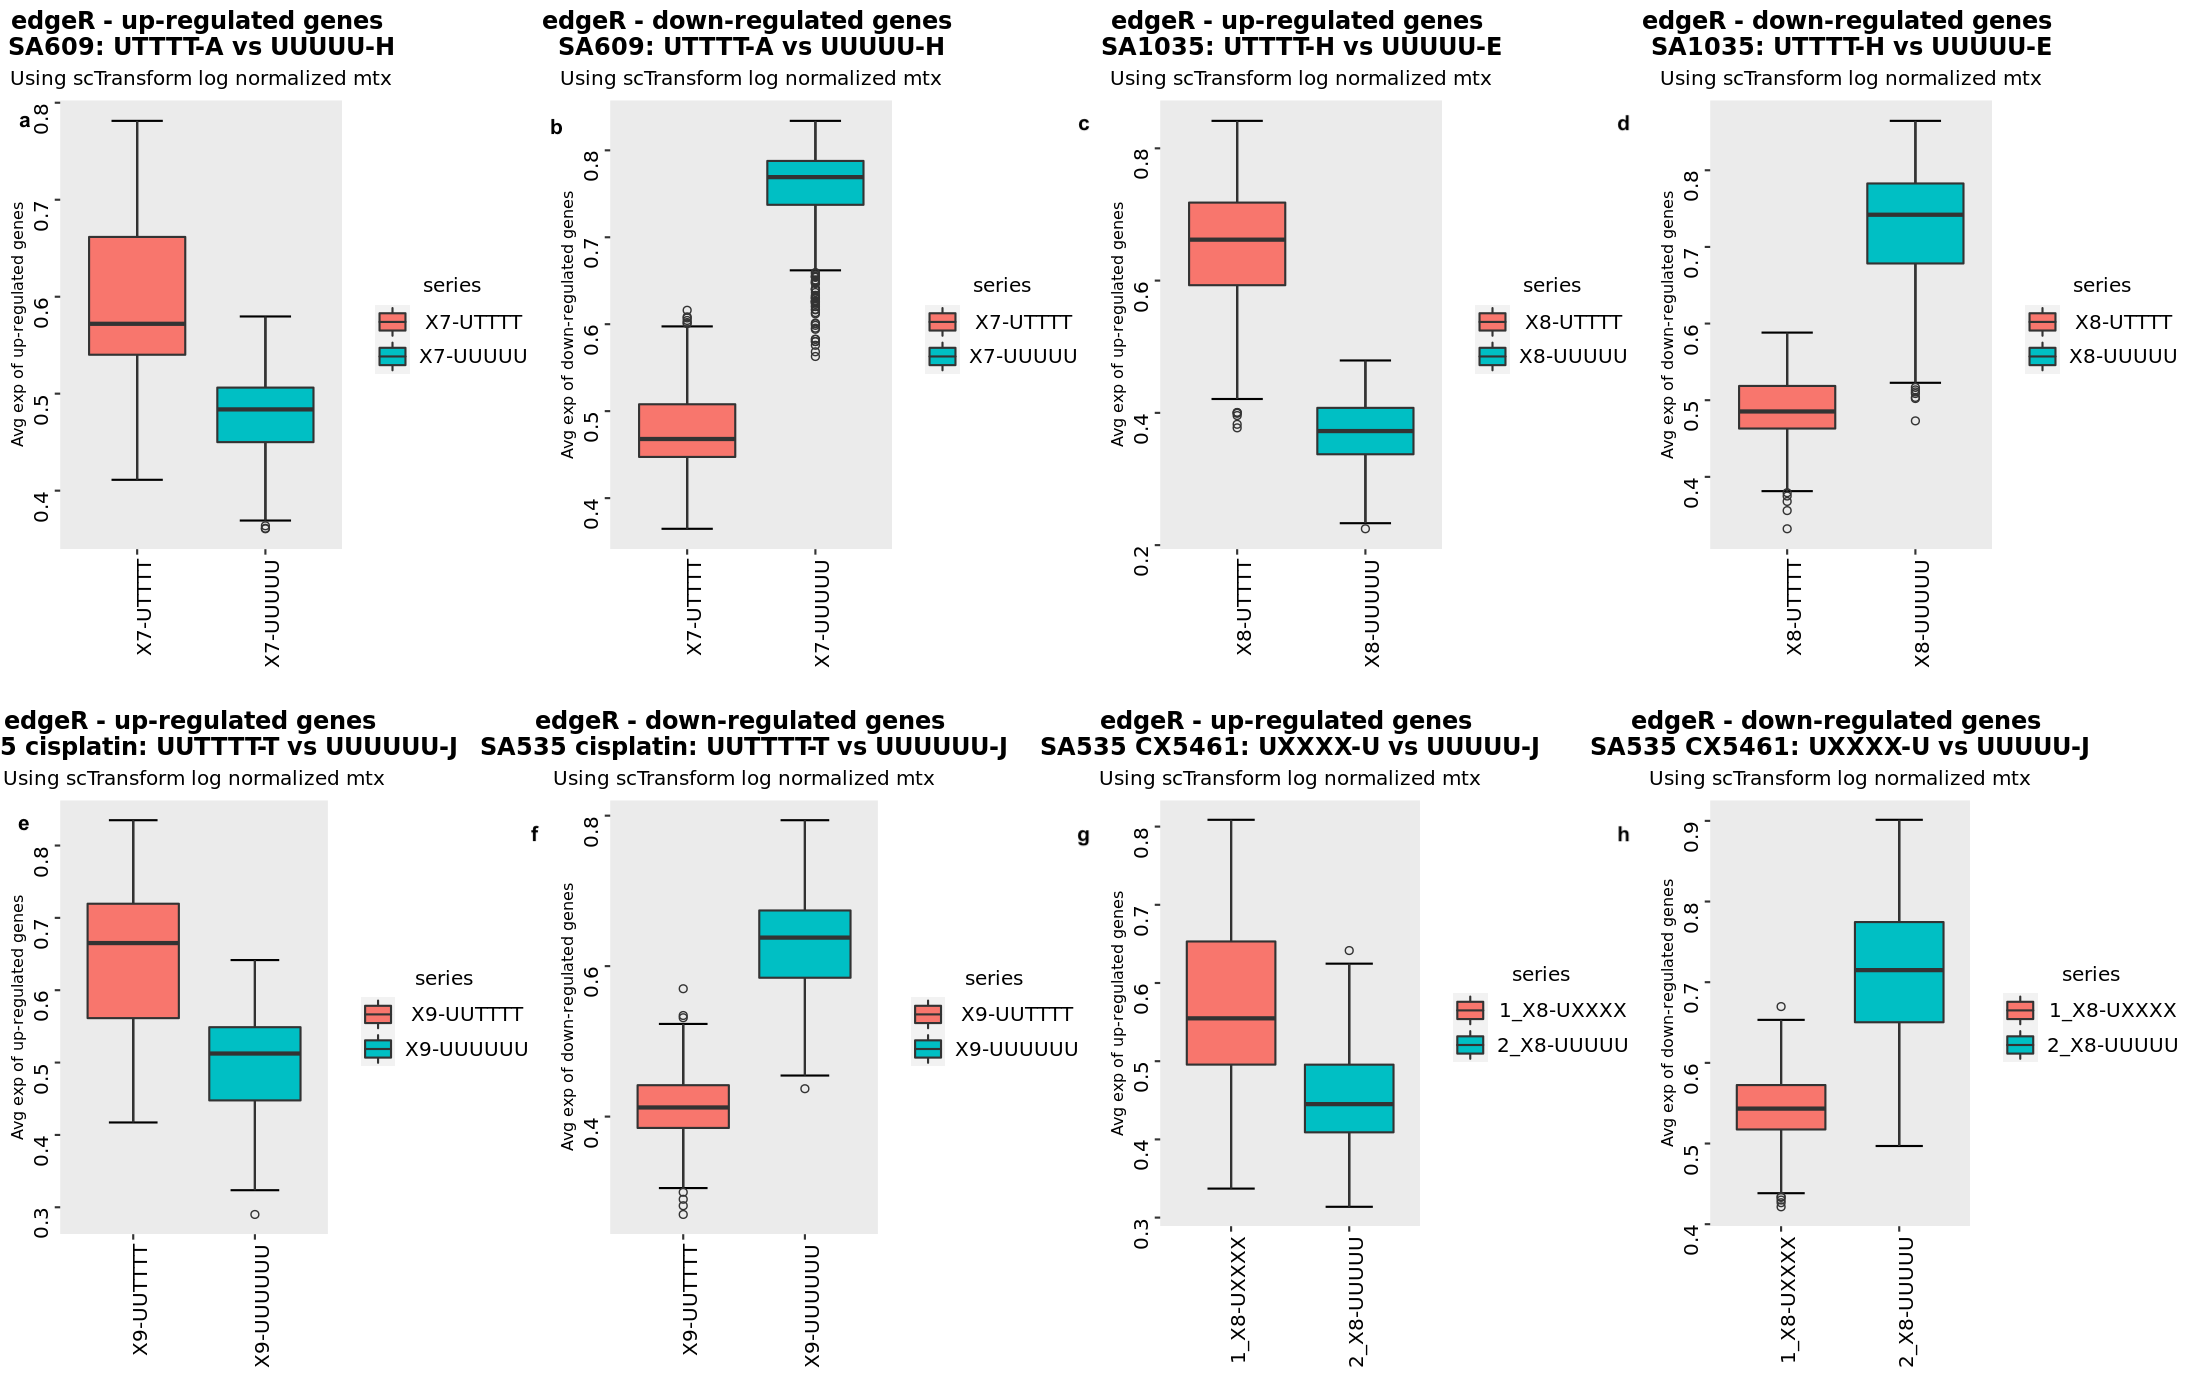
\includegraphics[width=\textwidth]{Figures/chap5/edgeRevaluation3series.png}
	
\caption[Evaluation of \texttt{edgeR} in all PDX timeseries data.]
	{\small
	\textbf{Evaluation of \texttt{edgeR} in all PDX timeseries data.}
	Box plots showing upregulated and downregulated differentially expressed genes in four TNBC timeseries PDX. Horizontal axis shows sample status and passage timepoint, where each `T' stands for one cycle of cisplatin and each `X' stands for one cycle of CX-5461. `U' stands for untreated timepoint. Vertical axis denotes average expression of genes.
	\textbf{(a)} TNBC-SA609 showing upregulated gene expression in 4 cycles treated resistant tumor (red) and sensitive tumor (blue). 
	\textbf{(b)} TNBC-SA609 showing down regulated gene expression in 4 cycles treated resistant tumor (red) and sensitive tumor (blue). 
		\textbf{(c, d)} Same as \textbf{(a, b)} but for TNBC-SA1035.
		\textbf{(e, f)} Same as \textbf{(a, b)} but for TNBC-SA535-Cisplatin treated.
		\textbf{(g, h)} Same as \textbf{(a, b)} but for TNBC-SA535-CX-5461 treated.
	}
	\label{fig:edgeRevaluation3series}
\end{figure}

%-------------------------------------------------------------



\begin{figure}
\centering
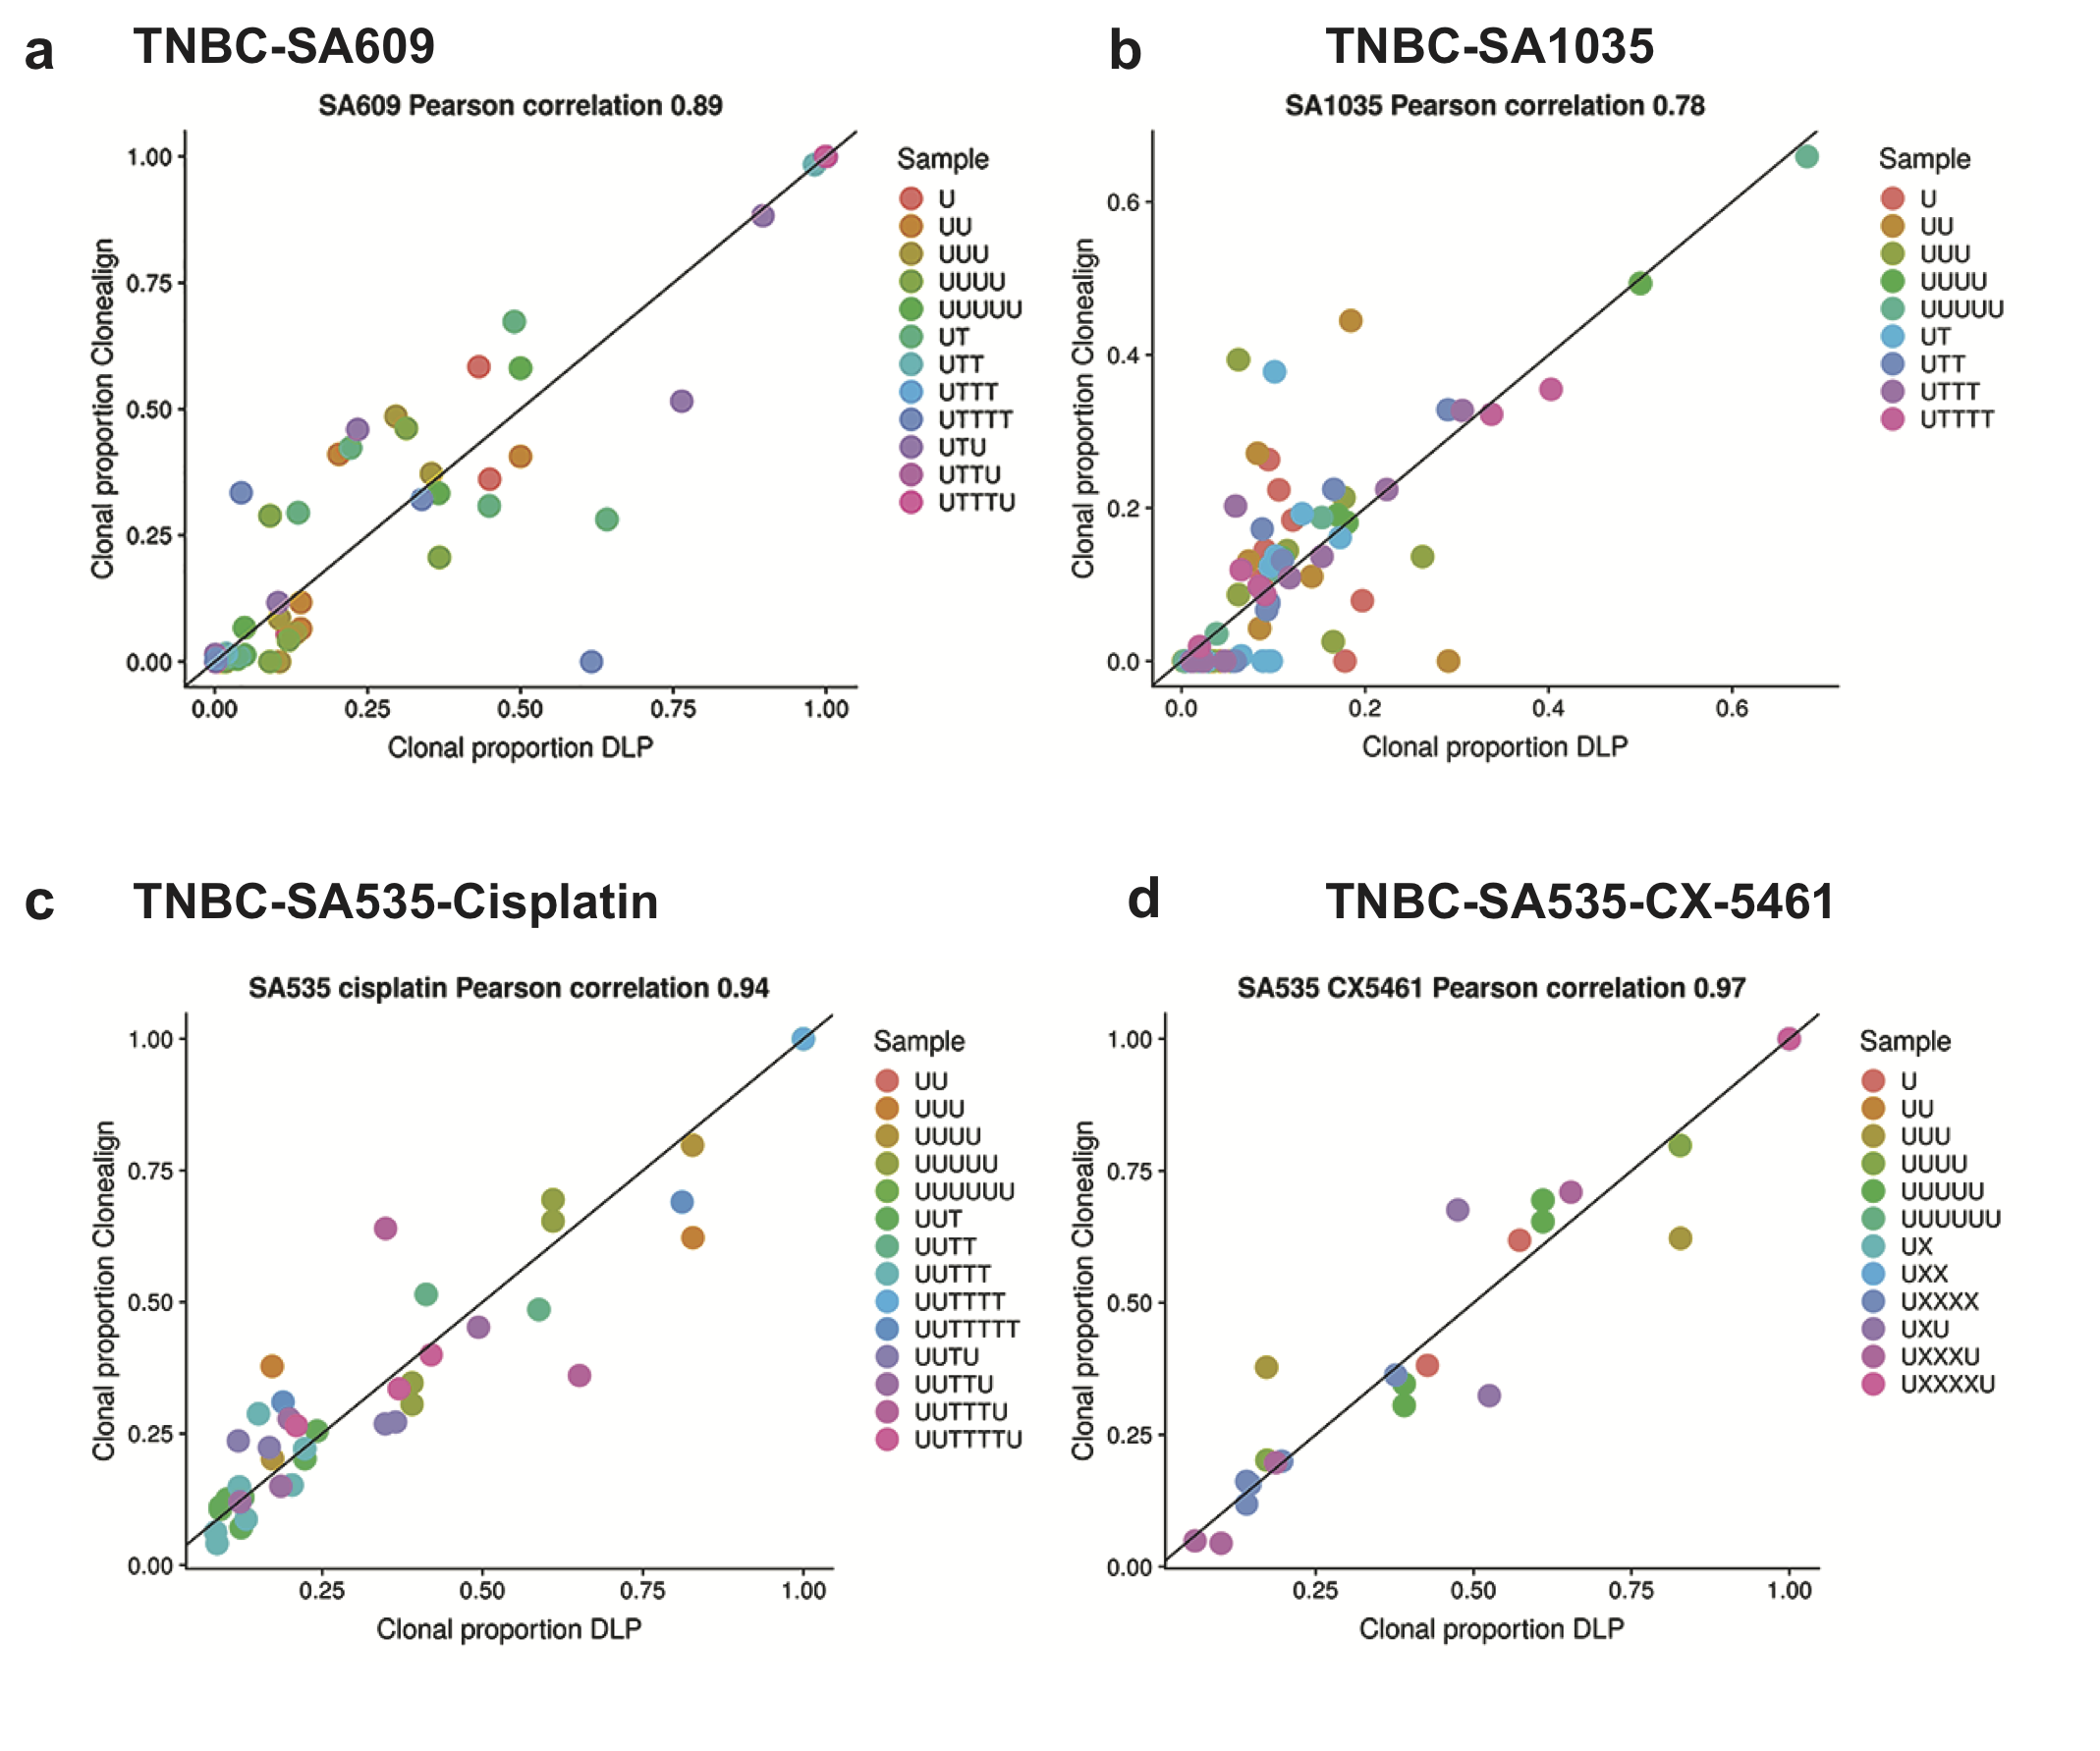
\includegraphics[width=\textwidth]{Figures/chap5/Clonealigncorrelation.png}
	
\caption[\texttt{clonealign} clonal proportions vs DLP+ clonal proportions]
	{\small
	\textbf{\texttt{clonealign}, clonal proportions vs DLP+ clonal proportions.}
	   Clonal proportions of scRNAseq  derived from \texttt{clonealign} estimates against CNA derived clones
	   \textbf{(a)} \texttt{clonealign} clonal proportions vs DLP+ clonal proportions of TNBC-SA609 PDX timeseries samples indicating positive correlation (Pearson correlation from $r \geq 0.89$).
	 \textbf{(b)} Same like \textbf{(a)} but for TNBC-SA1035 PDX and Pearson correlation is $r \geq 0.78$. \textbf{(c)} Same like \textbf{a} but for TNBC-SA535 PDX and Pearson correlation is $r \geq 0.94$ for cisplatin treated. \textbf{(d)} Same like \textbf{a} but for SA535 PDX and Pearson correlation is $r \geq 0.97$ with CX-5461 treated. Number of `T' indicates number of cycles of cisplatin while number of `X' indicates number of cycles of CX-5461.}
	 
	\label{fig:Clonealigncorrelation}
\end{figure}



%--------------------------------------------------------------------


\begin{figure}
\centering
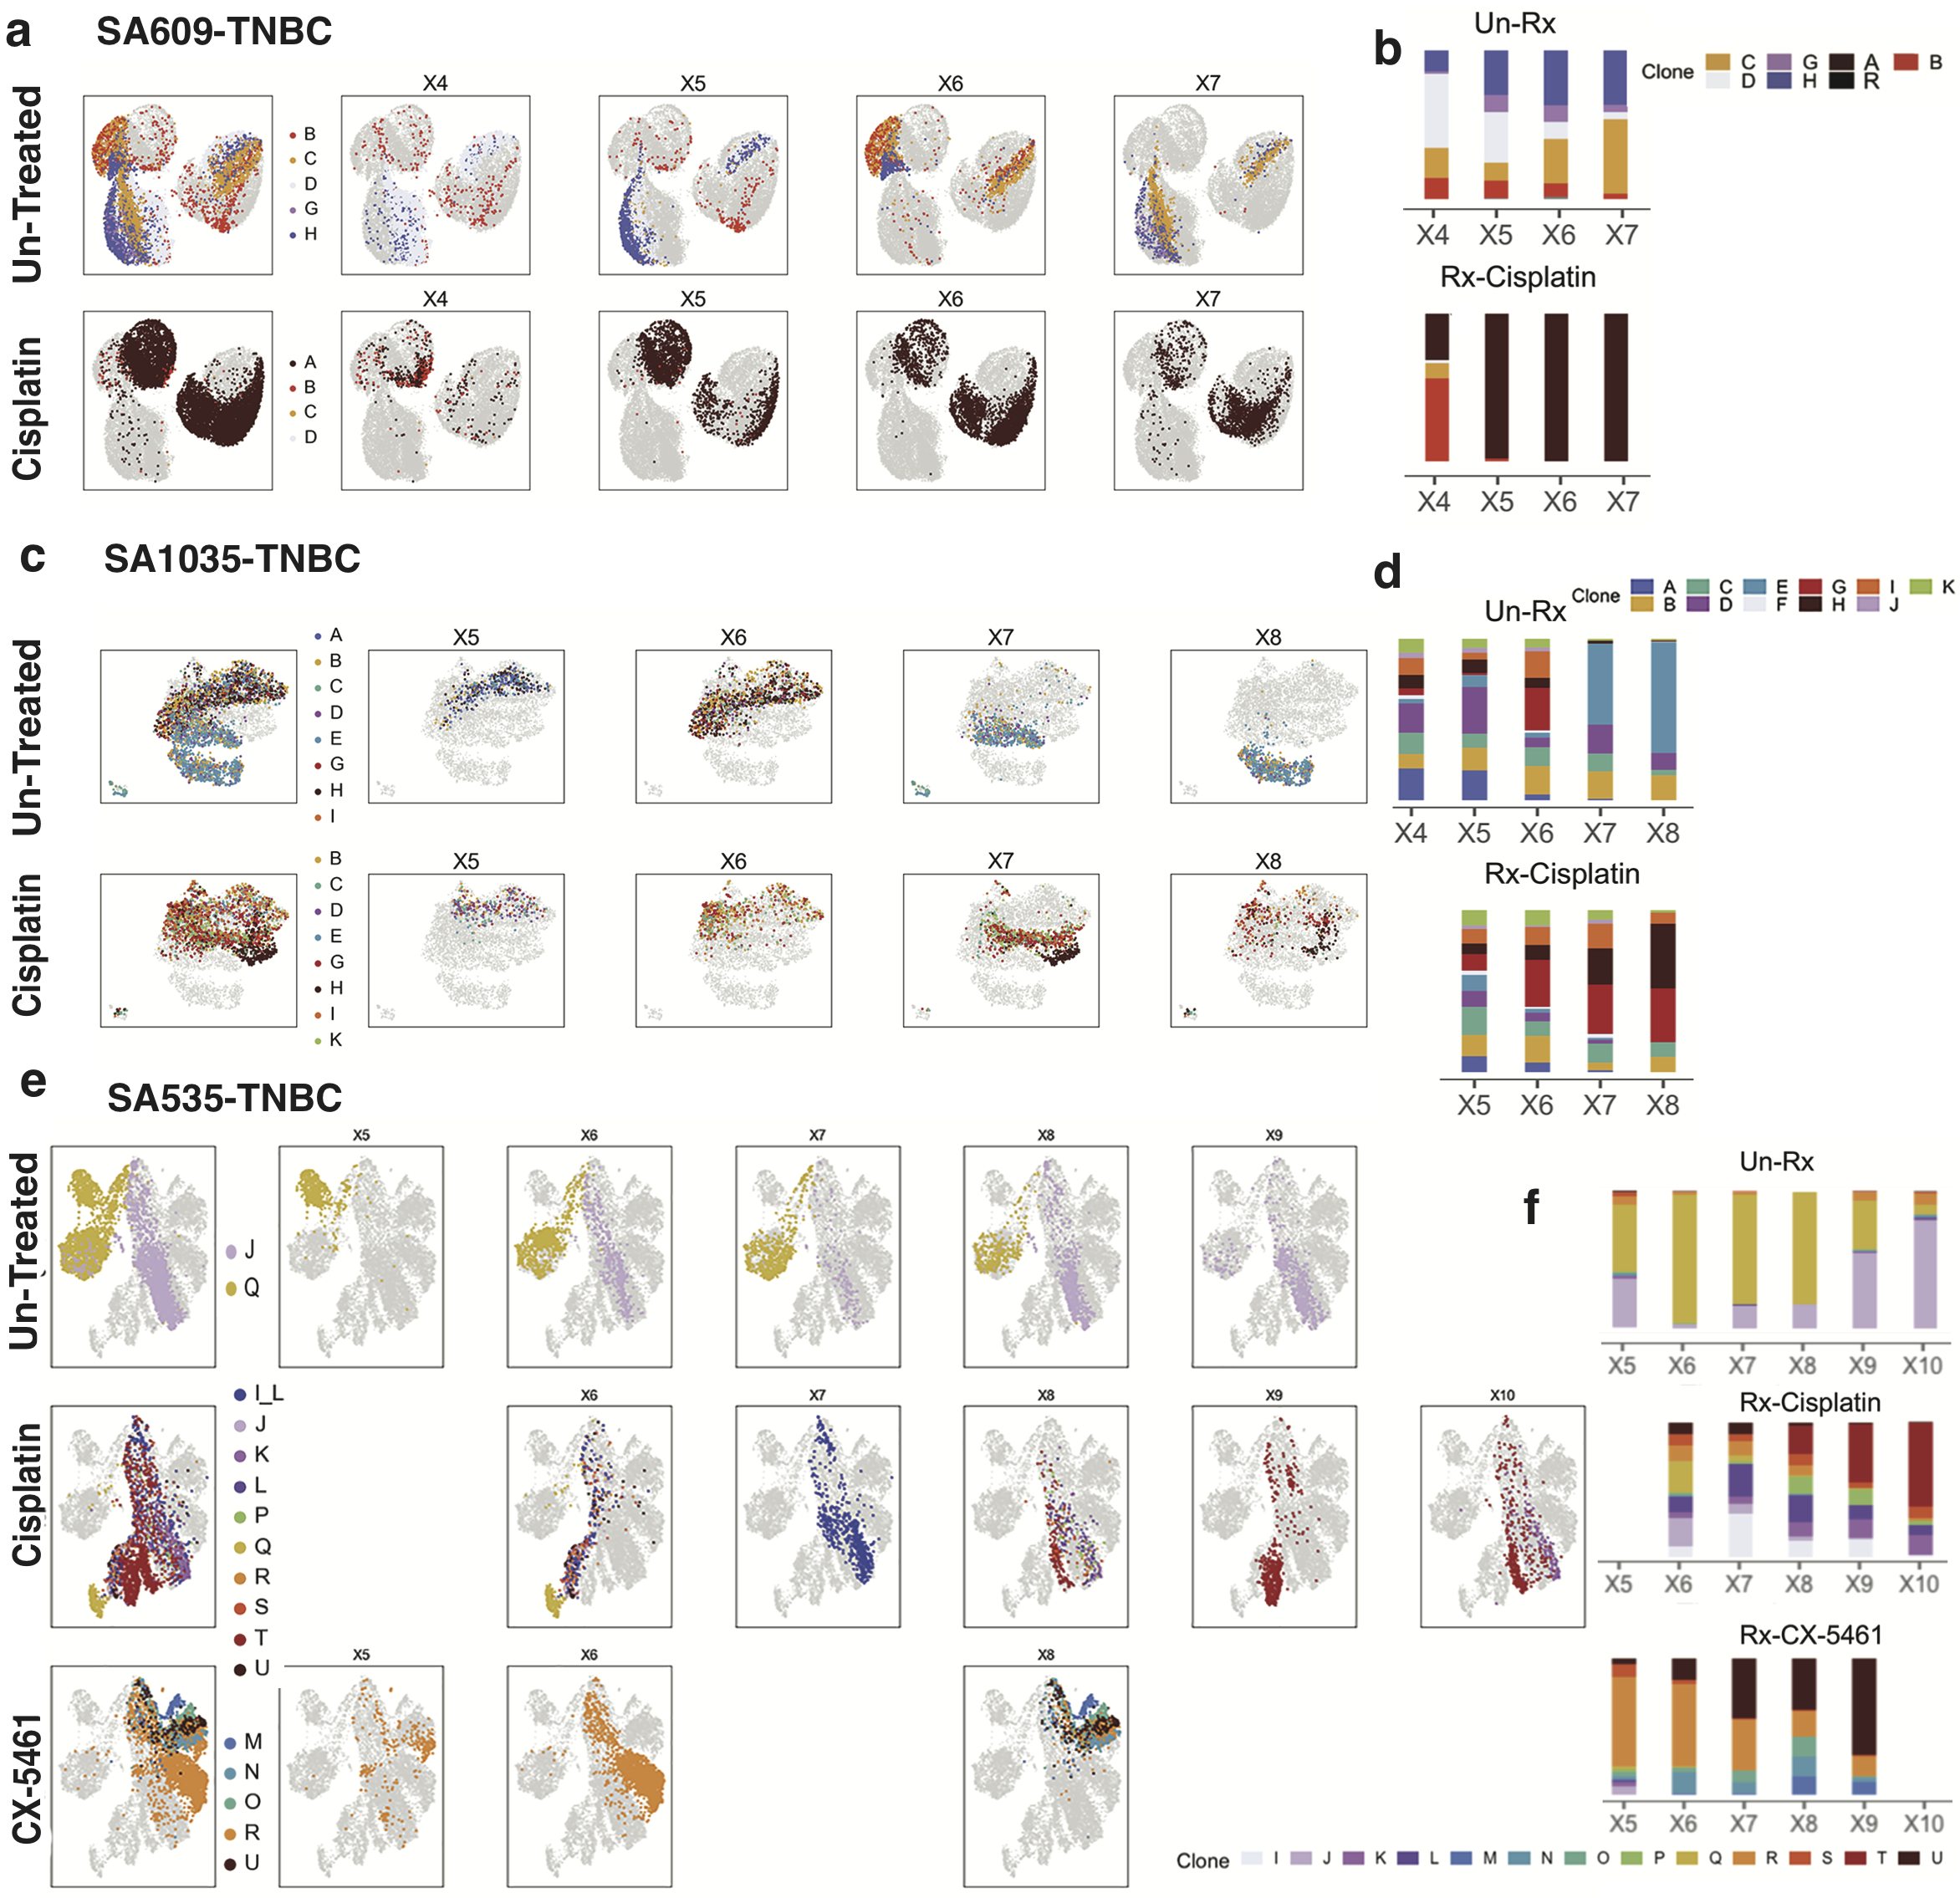
\includegraphics[width=\textwidth]{Figures/chap5/EmbeddingsRNA.png}
	
\caption[Gene expression impacts of clone-specific copy number profiles]
	{\small
	\textbf{Gene expression impacts of clone-specific copy number profiles.}
	    \textbf{(a)} Low dimensional \ac{UMAP} embeddings of matching scRNAseq libraries across the SA609 TNBC timeseries. Left top and bottom panels show untreated and treated complete embedding annotated with clonealign assignments and right all panels show the density of cell clusters over the timeseries X4-X7.
	     \textbf{(b)} Barplots to recall clonal proportion from DLP+ of TNBC-SA609 taken from previous chapter with and without drug. 
	     \textbf{(d)} Same like \textbf{(b)} but for TNBC-SA1035 PDX. \textbf{(e)} Same like \textbf{(a)} but for TNBC-SA535  from X5-X8. \textbf{(f)} Same like \textbf{c} but for SA1035. \textbf{(g)} Same like \textbf{a} but for SA535 PDX and Pearson correlation is 0.94 for cisplatin treated and 0.97 with CX-5461 treated. \textbf{(h)} Same like \textbf{b} but for TNBC-SA535 starting from X5-X9 (un-treated), X6-X10 (Cisplatin) and X5, X6, X8 (CX-5461).
	}
	\label{fig:EmbeddingsRNA}
\end{figure}

%----------------------------------------------------------------

\subsubsection{SCTransform performs more optimal normalization for Single cell RNAseq data in longitudinal \textit{in vivo} experiments}
 To discern the nature of single cell RNA sequencing data in longitudinal samples, we applied few comparative and diagnostic statistical tools to check the normalization and its effects in our datasets.
 House keeping genes were selected \cite{lin2019evaluating} and the mean expression was calculated in all timeseries of TNBC PDX. Mean gene expression was calculated in complete datasets to compare the raw data (\textbf{\autoref{fig:Comparisonofbatcheffects} a}) with twice scran \cite{lun2016pooling} \textbf{\autoref{fig:Comparisonofbatcheffects} b}, Seurat \cite{butler2018integrating} \textbf{\autoref{fig:Comparisonofbatcheffects} c} and SCTransform \cite{hafemeister2019normalization}. Normalization with SCTransform partially removed batch effects with small range of mean gene expression differences \textbf{\autoref{fig:Comparisonofbatcheffects} d}.

\subsubsection{Comparison of \texttt{edgeR} with SCTransform normalization for downstream data analysis}
Differential expression (DE) analysis is the most important part in order to detect change in gene expression due to drug exposure. A benchmark study evaluated eleven methods \cite{soneson2013comparison} for differential expression analysis of RNA-seq transcriptomic data, and show that \texttt{edgeR} is one of the best method with high accuracy of differential expressed genes detection while showing low false discovery rated compared to other methods. As this method focus on quantifying the relative changes in expression level between groups of cells rather than providing a normalized expression data and takes raw data counts instead of normalized logarithm counts, we sought to evaluate whether differentially expressed (DE) genes that are detected by \texttt{edgeR} are true DE genes or a false positive detected genes due to technical effects of data handling.

To prove that edgeR provide results with accuracy, based on the list of up-regulated and down-regulated genes (obtained by applying \texttt{edgeR} function), we estimated the mean expression of these genes between conditions using SCTransform log normalized gene expression matrix. Normalized gene expression matrix produced from SCTransform was used to evaluate the output of differentially expressed (DE) genes from \texttt{edgeR}. It is expected that DE up-regulated genes in the resistant clone (treated sample) would display a significantly high level of normalized expression as compared to the sensitive clone (untreated sample). If a gene is a false positive detected gene, the normalized gene expression would not be significantly expressed between the samples. Same assumption was applied to differentially expressed down-regulated genes. 

 Therefore, we evaluated the performance of \texttt{edgeR} for DE genes detected in all four timeseries datasets taking SCTransform normalized matrix.
 we estimated average the \texttt{edgeR} results of up-regulated and  down-regulated genes from DE comparison of resistant clone compared to the sensitive clones. Quantifying the results from TNBC-SA609 showed that DE up-regulated genes expression in the resistant clone (median value 0.57, min: 0.54, max:0.66 - average SCTransform normalized expression of all cells in resistant Clone A) is significantly greater than in the sensitive Clone H in untreated cells group (median value 0.46, min: 0.45, max:0.49) \textbf{\autoref{fig:edgeRevaluation3series} a}. 
 
 Similarly, for down-regulated genes in TNBC-SA609, the resistant Clone A (median value 0.48, min: 0.47, max:0.5 - average SCTransform normalized expression of all cells in first group) is significantly lower than the sensitive clone H containing timepoint (median value 0.76, min: 0.74, max:0.79) \textbf{\autoref{fig:edgeRevaluation3series} b}. Same results were deduced from TNBC-SA1035, TNBC-SA535 (cisplatin) and TNBC-SA535 (CX-5461) \textbf{\autoref{fig:edgeRevaluation3series} c-h}. 
 
 In summary, based on the mean expression of obtained DE genes from SCTranform normalized matrix, it proved that \texttt{edgeR} could be used for accurate DE genes detection and is the right choice for our dataset.

%-----------------------------------------------------------------


\subsection{Clone-specific genotypes underpin clone-specific gene expression programs}
Next, we profiled the impact of clone specific gene expression changes as a higher order representation of phenotypic properties. We tested if the genotypes of high fitness clones exhibited changes in their transcriptional program, with scRNAseq performed on matched aliquots of same samples sequenced using DLP+ on the serially passaged TNBC PDX as mentioned previously (\textbf{\autoref{fig:RNAsampletree}}.

\subsubsection{Copy number defined clones and scRNAseq expression revealed high concordance across PDX timeseries}
  %In our approach, we assume clones are defined through grouped cell subsets which share to a first approximation similar genomic copy number structure \cite{laks2019clonal}(e.g., through phylogenetic reconstruction or dimensionality reduction). 
 To assess the correlation of DLP+ defined clonal fractions (chapter 4) at each time point in single cell RNA space, we applied \texttt{clonealign}, a statistical method, \cite{campbell2019clonealign} to reveal clone-specific phenotypic properties across all selected samples.
  Each point is taken as the proportion of DLP+ cells in a clone horizontal axis versus the proportion of the scRNAseq cells in the same clone. The  correlation for all clones were then calculated by using Pearson correlation coefficient formula. The heat maps of TNBC-SA609 PDX \textbf{(\autoref{fig:mediangenotypes}}) exhibit more complex heterogeneity at copy number space along with structural genomic rearrangements as compared to TNBC-SA1035 PDX. The results depicted that DLP+ and \texttt{clonealign}, the  clone abundance measures were positively correlated across all libraries \textbf{(\autoref{fig:Clonealigncorrelation})}. Importantly, TNBC-SA535 treated with cisplatin, 14 tumors (14 libraries), presented the high confidence correlation with Pearson correlation 0.94 (p-value$< 10^{-18}$), followed by its CX-5461 treated series 12 tumors (12 libraries), presenting Pearson correlation of 0.97 (p-value$< 10^{-15}$) \textbf{\autoref{fig:Clonealigncorrelation} c, d}. However, TNBC-SA609 PDX timeseries, 12 tumors (12 libraries) presented a Pearson correlation coefficient of 0.89 (p-value $< 10^{-16}$) \textbf{(\autoref{fig:Clonealigncorrelation} a)} and TNBC-SA1035 PDX, 9 tumors (9 libraries), with Pearson correlation of 0.78 (p-value$< 10^{-18}$) \textbf{(\autoref{fig:Clonealigncorrelation} b)}.
  
  
\subsubsection{Single cell RNA embeddings exhibit relatively visible clone structure with residual batch effects}
%Single cell RNAseq clusters exhibit relatively monomorphic pattern of globalexpression over time that tracked clone assignments

Having made the assignments of cells to clones, next, we sought to visualize the data using UMAP \cite{becht2019dimensionality}, dimensionality reduction method, to aggregate cells into treated and untreated subpopulations while retaining the relationship between subpopulations. We found that scRNAseq embeddings displayed a dynamic pattern of global expression over time with and without treatment, which tracked with clone assignments indicating co-variation of transcriptional properties with clonal abundance. UMAP visualization of clusters identified Clone H cells clusters together at the last time point along with Clone C, in untreated setting and Clone A cells clusters together \textbf{\autoref{fig:EmbeddingsRNA} a}, in the cisplatin treated series of TNBC-SA609 PDX, purified over time matching their genomically defined counterparts \textbf{(\autoref{fig:EmbeddingsRNA} b)}. Similarly, Clone E in untreated and Clone H in treated timeseries of TNBC-SA1035  \textbf{(\autoref{fig:Clonealigncorrelation} c)}, clustered uniquely at the later time points. \textbf{\autoref{fig:EmbeddingsRNA} d} reminding the clonal prorportions at each time point in DLP+ emerging with and without treatment from chapter 4 in TNBC-SA1035. 

TNBC-SA535 PDX all three arms of untreated, treated with cisplatin and treated CX-5461, exhibited aggregation of similar patterns of cell clusters that favours emerging of genomic clones in their respective series \textbf{\autoref{fig:EmbeddingsRNA} e,f}. Clone J (purple), in untreated control timeseries \textbf{(\autoref{fig:EmbeddingsRNA} e, top panel)}, Clone T (red), in cisplatin treated \textbf{(\autoref{fig:EmbeddingsRNA} e, middle panel)}, and clone U (dark brown) in CX-5461 treated \textbf{(\autoref{fig:EmbeddingsRNA} e, lower panel)}. They are showing approximately similar proportions with respect to other clones as observed in DLP+ (\textbf{\autoref{fig:EmbeddingsRNA} f}).

%------------------------------------------------------------------

\begin{figure}
\centering
  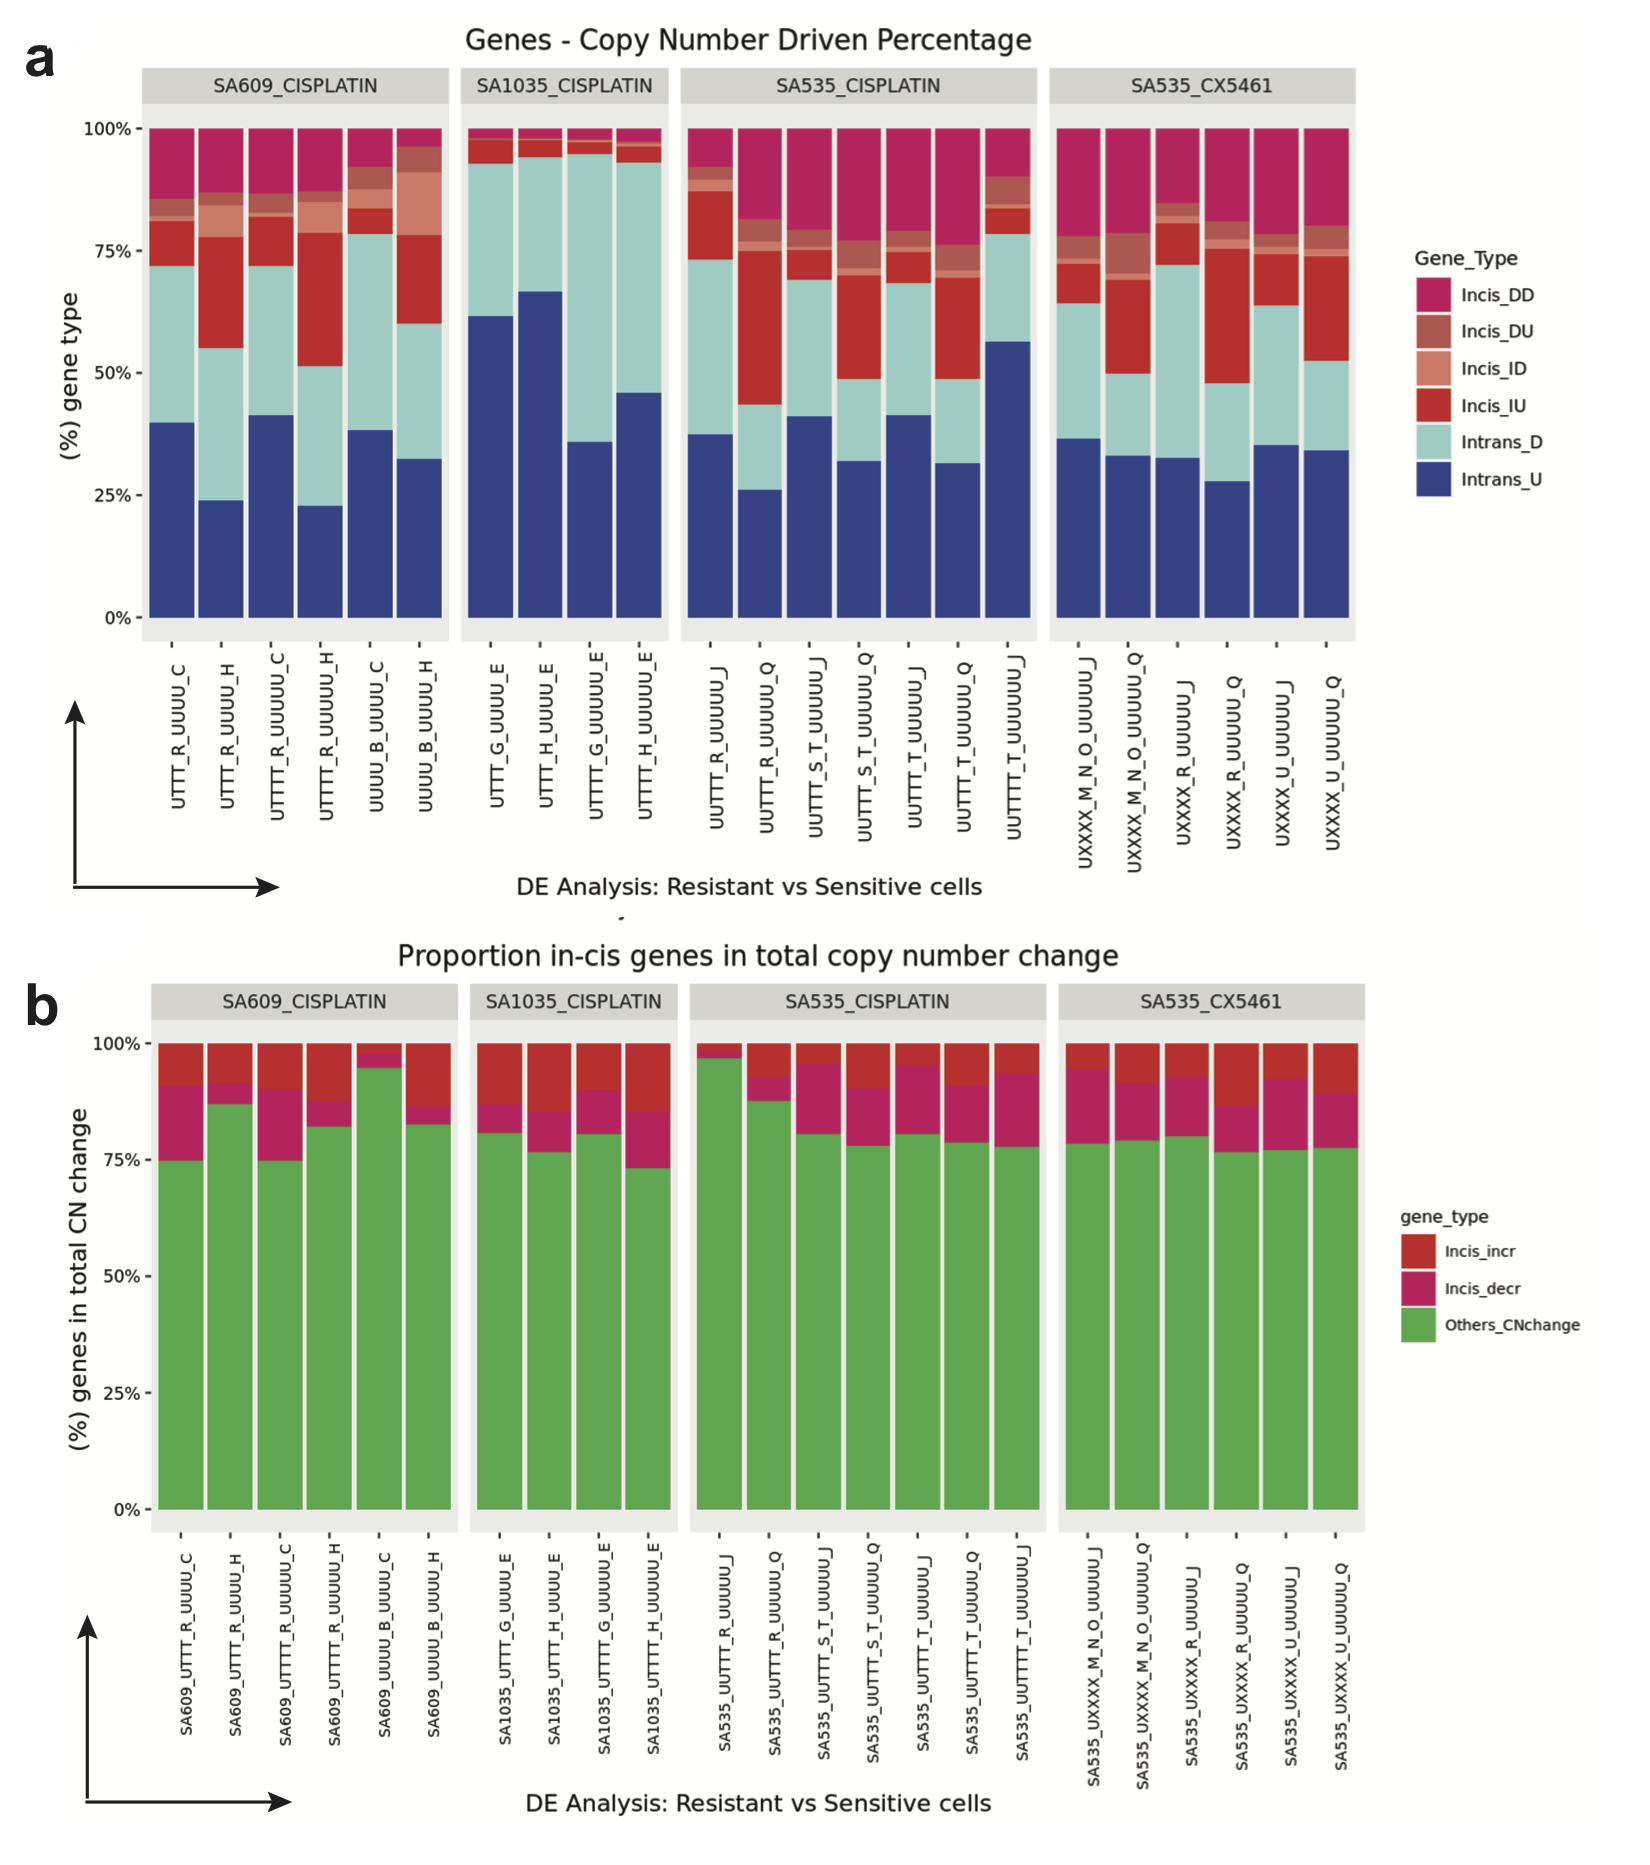
\includegraphics[width=\textwidth]{Figures/chap5/fig4Summaryincistrans.png}
	
\caption[Summary proportion of \textit{in cis} and \textit{in trans} regulated gene expression in scRNAseq data]
	{\small
	\textbf{Summary proportion of \textit{cis} and \textit{trans} regulated gene expression in scRNAseq data.}
	   Horizontal axis shows differential expression between two selected clones from all the three PDX treated and un-treated timeseries. Vertical axis gives percentages of genes.  \textbf{(a)}  Red and pink bars represent \textit{in cis} change in expression in both panels, and blue bars represent \textit{in trans} regulated gene expression. \textbf{(b)} Percentage of increased or decreased genes in total copy number change.
	     
	}
	\label{fig:fig3Summaryincistrans}
\end{figure}

%---------------------------------------------------------------

\subsection{Quantitative single cell gene expression analysis unravels the rates of \textit{in cis} and \textit{in trans} components}

It is broadly acknowledged that somatic CNV is highly associated with the development and progression of numerous cancers by influencing gene expression level \cite{yang2017prame, gut2018sox2}. 
Here, we investigated as to how much of the proportions of DE genes from resistant and sensitive clones are \textit{in cis} and \textit{in trans} regulated genes. 

To calculate the percentage of genes presenting \textit{in cis} or \textit{in trans} regulatory effects, the differential expression single cell RNAseq data was decomposed into \textit{cis}, where the gene expression that is following the change in copy number and \textit{trans}, where it is independent.

\subsubsection{Copy number change in clones displayed a phenotypic expression}
%{Differential gene expression between resistant and sensitive clones exhibit high \textit{in trans} proportion.}

To determine how much of the transcriptome is modulated by \textit{in cis} and \text{in trans}, first, the differential expression \ac{DE} analysis between resistant and sensitive clones  (\textbf{\autoref{tab:Listofresistantandsensitiveclones}}) was done.  Some of the selected clones that were closely related to the resistant clones or having second highest fitness coefficients in DLP+ data from chapter 4, were also added to DE analysis from each of the time series PDX using \texttt{edgeR} \cite{robinson2010edger}. 
Next, we classified these genes into upregulated with increase in copy number (incis\_IU) and downregulated (incis\_DD) with decrease in copy number or upregulated with decrease in copy number (incis\_DU) or downregulated with increase in copy number (incis\_ID), from one clone to another, as mentioned in the legend of \textbf{\autoref{fig:fig3Summaryincistrans} a}.

From HMMcopy output of segment copy number position (chromosome start and end), we get gene coordinates by mapping gene segment positions with reference database of known genes for human  \cite{carlson2015txdb}. First, we identified overlapping positions between chromosome segments and known genes, then we assigned those segments to an ensemble gene ID \cite{rainer2019ensembldb} of the  selected \ac{DE} of clones across all timeseries and calculated their number and percentages in each PDX timeseries  \textbf{\autoref{tab:DEpercentageincisintrans}}. Notably, we found that the overall number of \textit{in trans} genes were higher as compared to \textit{in cis}, which is supporting previously reported results \cite{shao2019copy}. Our dataset showed that around 20-50\% of transcriptome is modulated \textit{in-cis} by \ac{CNA} depicting that copy number altered clones have a phenotypic expression.

%------------------------------------------------------

% Please add the following required packages to your document preamble:
% \usepackage{graphicx}
% \usepackage{lscape}
\begin{landscape}
\begin{table} 
\centering
\caption{Summary of \textit{in cis} and \textit{in trans} percentages (\%) of differentially expressed genes}
\resizebox{\textwidth}{!}{%
\begin{tabular}{|l|p{4em}|p{4em}|p{4em}|p{4em}|p{4em}|p{4em}|}
  \hline
\ac{DE}-scRNAseq between clones &
  In\_cis\_Decrease\_DownRegulated \% &
  In\_cis\_Decrease\_UpRegulated \% &
  In\_cis\_Increase\_DownRegulated \% &
  In\_cis\_Increase\_UpRegulated \% &
  In\_trans\_DownRegulated \% &
  In\_trans\_UpRegulated \% \\
    \hline
SA609-UUUU-A\_vs\_UUUU-C         & 7.9  & 4.4 & 4   & 5.2  & 40.1 & 38.4 \\
SA609-UUUU-A\_vs\_UUUU-H         & 3.5  & 5.1 & 13  & 17.5 & 27.7 & 33.2 \\
SA609-UTTT-A\_vs\_UUUU-C         & 14.4 & 3.3 & 1.1 & 9.3  & 32.1 & 39.8 \\
SA609-UTTT-A\_vs\_UUUU-H         & 13   & 2.5 & 6.5 & 22.5 & 31.3 & 24.2 \\
SA609-UTTTT-A\_vs\_UUUUU-C       & 13.2 & 3.8 & 0.9 & 10.1 & 30.5 & 41.5 \\
SA609-UTTTT-A\_vs\_UUUUU-H       & 12.8 & 2.2 & 6.1 & 27.1 & 28.7 & 23   \\
SA1035-UTTTT-G\_vs\_UUUUU-E      & 1.8  & 0.2 & 0.4 & 2.3  & 59.2 & 36.2 \\
SA1035-UTTTT-H\_vs\_UUUUU-E      & 2.6  & 0.5 & 0.5 & 3.3  & 47.2 & 45.8 \\
SA1035-UTTT-G\_vs\_UUUU-E        & 1.6  & 0.1 & 0.1 & 4.8  & 31.5 & 61.9 \\
SA1035-UTTT-H\_vs\_UUUU-E        & 1.9  & 0.3 & 0.3 & 3.4  & 27.4 & 66.7 \\
SA535\_UUTTTT-T\_vs\_UUUUUU-J     & 9.7  & 5.6 & 0.3 & 3.2  & 22.8 & 58.3 \\
SA535\_UUTTT-T\_vs\_UUUUU-J       & 20.9 & 3.4 & 0.2 & 4.5  & 27.6 & 43.3 \\
SA535\_UUTTT-S\_T\_vs\_UUUUU-J       & 20.7 & 3.4 & 0.2 & 4.4  & 28.3 & 43   \\
SA535-UUTTT-R\_vs\_UUUUU-J       & 7.9  & 2.5 & 1.5 & 12.3 & 36.8 & 39.1 \\
SA535\_UUTTT-T\_vs\_UUUUU-Q       & 22.5 & 4.9 & 1.5 & 20.7 & 18.4 & 32   \\
SA535-UUTTT\_S\_T\_vs\_UUUUU-Q    & 21.7 & 5.2 & 1.4 & 21.2 & 18.1 & 32.4 \\
SA535-UUTTT-R\_vs\_UUUUU-Q       & 16   & 4.4 & 1.8 & 31.5 & 19.9 & 26.4 \\
SA535-UXXXX-U\_vs\_UUUUU-J       & 21.5 & 2.8 & 0.6 & 8.8  & 29.2 & 37.1 \\
SA535-UXXXX-U\_vs\_UUUUU-Q       & 18.1 & 4.4 & 1.6 & 21.4 & 20.1 & 34.5 \\
SA535-UXXXX-R\_vs\_UUUUU-J       & 15.3 & 2.4 & 0.6 & 7    & 40.4 & 34.3 \\
SA535-UXXXX-R\_vs\_UUUUU-Q       & 17.1 & 3.4 & 1.9 & 27.5 & 21.8 & 28.2 \\
SA535\_UXXXX\_M\_N\_O\_vs\_UUUUU-J & 22.1 & 4.3 & 0.4 & 6    & 28.5 & 38.7 \\
SA535-UXXXX-M\_N\_O\_vs\_UUUUU\_Q & 19.7 & 7.7 & 1.3 & 19.3 & 18.6 & 33.5 \\
  \hline
 \end{tabular}%
 }
\label{tab:DEpercentageincisintrans}
\end{table}
\end{landscape}

%------------------------------------------------------------------


%------------------------------------------------------------



\subsubsection{Global copy number change between the genomes of two clones}

To estimate approximately how much of the genome manifest change in copy numbers from one clone to other in our data sets, we computed median genotype profiles of the clones for which we calculated \ac{DE} above.

Total of 22,326 segment positions, from each DE analysis, were mapped. In each pair wise comparison of clones, we captured all segment copy number position where there is a change in copy number values. So \textit{in cis} gene is differentially expressed gene in scRNAseq analysis and coupled with change in copy number at the same position of genome HMM copy number segment positions. Approximately 9000 segments had copy number changes between two clones, and $>$2000 position intersect with scRNAseq genes.

In other words, the average change in copy number between the genomes of two clones in our data set was found to be around 41\%. Out of this, approximately 28\% of the transcriptome is coupled with change in copy number state between clones at these segment positions. It involves either increase in expression with copy number gain or decrease in expression with copy number loss, shown in pink and red for \textit{in cis} and rest of around 72\% of the copy number change was not associated with change in expression shown as green in \textbf{(\autoref{fig:fig3Summaryincistrans} b)}. Detailed percentages of \textit{in cis} and others are mentioned in \textbf{\autoref{tab:copynumberchange}}.

%------------------------------------------------------------------
% Table generated by Excel2LaTeX from sheet 'copy number change'
 \begin{table}[htbp]
   \centering
   \caption{Percent change of copy number from one clone to another}
     \begin{tabular}{|l|l|l|l|}
       \hline
     Samples & \multicolumn{1}{|l}{Percent\_incis\_incr} & \multicolumn{1}{|l}{Percent\_incis\_decr} & 
     \multicolumn{1}{|l|}{Percent\_others} \\
      \hline
     SA609-UUUU-B\_to\_UUUU-C & 2.25 & 3.01 & 94.74 \\
     SA609-UUUU\_B\_to\_UUUU-H & 13.51 & 3.82 & 82.67 \\
     SA609-UTTT\_A\_to\_UUUU-C & 9.35 & 15.91 & 74.74 \\
     SA609-UTTT\_A\_to\_UUUU-H & 8.55 & 4.57 & 86.88 \\
     SA609-UTTTT\_A\_to\_UUUUU-C & 9.96 & 15.35 & 74.69 \\
     \textbf{*}SA609-UTTTT\_A\_to\_UUUUU-H & 12.27 & 5.54 & 82.19 \\
     SA1035-UTTTT\_G\_to\_UUUUU-E & 12.15 & 9.19 & 78.66 \\
     \textbf{*}SA1035-UTTTT\_H\_to\_UUUUU-E & 14.66 & 12.05 & 73.29 \\
     SA1035-UTTT\_G\_to\_UUUU-E & 16 & 5.63 & 78.37 \\
     SA1035-UTTT\_H\_to\_UUUU-E & 14.66 & 8.69 & 76.65 \\
     \textbf{*}SA535-UUTTTT\_T\_to\_\_UUUUUU-J & 4.5 & 19.81 & 75.69 \\
    \textbf{*}SA535-UUTTT\_T\_to\_UUUUU-J & 3.59 & 18.63 & 77.78\\
     SA535-UUTTT\_S\_T\_to\_UUUUU-J & 3.51 & 18.53 & 77.96 \\
     SA535-UUTTT\_R\_to\_UUUUU-J & 2.03 & 1.54 & 96.43 \\
     SA535-UUTTT\_T\_to\_UUUUU-Q & 9.89 & 12.2 & 77.91 \\
     SA535-UUTTT\_S\_T\_to\_UUUUU-Q & 10.42 & 12.44 & 77.14 \\
     SA535-UUTTT\_R\_to\_UUUUU-Q & 7.92 & 4.85 & 87.23 \\
\textbf{*}SA535-UXXXX\_U\_to\_UUUUU-J & 7.19 & 18.45 & 74.36 \\
     SA535-UXXXX\_U\_to\_UUUUU-Q & 11.84 & 11.59 & 76.57 \\
     SA535-UXXXX\_R\_to\_UUUUU-J & 6.8 & 15.94 & 77.26 \\
     SA535-UXXXX\_R\_to\_UUUUU-Q & 14.37 & 10.06 & 75.57 \\
     SA535-UXXXX\_M\_N\_O\_to\_UUUUU-J & 4.53 & 18.69 & 76.78 \\
     SA535-UXXXX\_M\_N\_O\_to\_UUUUU-Q & 9.27 & 12.36 & 78.37 \\
   \hline 
   
 \end{tabular}%
\label{tab:copynumberchange}%

  \small\textbf{(* Resistant vs sensitive clones at the last time point of treatment cycle)}.
\end{table}%

%------------------------------------------------------------------

\subsubsection{Differential expression analysis displayed two fold  magnitude differences on both sides}
To get the idea of the magnitude of expression differences for most of up and down regulated genes, between the resistant and sensitive clones, we explored \ac{DE} with respect to their regulation \textit{in cis} and \textit{in trans}. In all the comparisons in 4 timeseries TNBC PDX, the magnitude of differentially expressed genes were found to be modestly equal on both up and down regulated sides. Majority of them were in the range of log2 fold change both in positive and negative directions. Furthermore, the colour coding in \textbf{\autoref{fig:Volcanoes4plots}}.

\subsubsection{Differential expression analysis of resistant and sensitive clones deciphers cancer related genes}
 Next, we investigated the proportions and types of genes that are upregulated in resistant clones in each of the treated PDX series.
 
 In TNBC-\textbf{SA609} PDX, pairwise comparisons of clone-specific differential gene expression, between resistant clone A and sensitive clone H (FDR$<$0.01, p$<$0.05), identified 922 genes having clone specific copy number increase in expression \textit{(incis\_IU)}, whereas, 435 genes were downregulated with decrease in copy number \textit{(incis\_DD)}. However, 975 genes were downregulated and 783 were upregulated independent of change in copy number ( \textit{in trans}) \textbf{(\autoref{fig:Volcanoes4plots} a}). 
 %The Manhattan plot establishing the increase and decrease in copy number between clones at that genomic position and its respective change in gene expression \textbf{(\autoref{fig:fig:Volcanoes4plots} a, right)}.
 
Amidst the upregulated \textit{in cis}, some known cancer promoting genes were detected, for example,  \textit{\textbf{HSPA1}} \cite{zoppino2018comprehensive},  \textit{\textbf{TCF4}} \cite{ravindranath2011wnt}, \textit{\textbf{NDUF}} \cite{li2015down}, 
\textit{\textbf{PTN}} \cite{huang2018chemotherapy},        
\textit{\textbf{ID4}} \cite{donzelli2018expression}, 
\textit{\textbf{RAC3}} \cite{donnelly2017rac3}. Many of them are not well studied in breast cancers and could be used as a potential candidates for comprehensive research \textbf{\autoref{tab:top20SA609upregulated}.}
Moreover, \textit{in cis} downregulated genes includes genes that have role in tumor suppression, for example, \textit{\textbf{OSR2}}, is a known tumor suppressor in gastric and lung cancer \cite{otani2014odd,wang2018odd}. Other genes including, \textit{\textbf{DYRK4}}, found to be downregulated in our data, is a key regulator of p53, and phosphorylates it at Ser46 to induce apoptosis in response to DNA damage \cite{yoshida2019multiple}, \textit{\textbf{POLR2K}} is a candidate biomarker for predicting breast cancer immunotherapy \cite{lopez2020prediction}. Another gene, \textit{\textbf{PRRX1}} is known to predict poor prognosis in hepatocellular carcinoma via the p53-dependent signaling pathway in hepatocellular carcinoma \cite{fan2017downregulation}. Furthermore,  
\textit{\textbf{KLF6}} is found to be among the upregulated genes, which is associated with poor prognosis in prostate, lung, ovarian cancer and 
breast cancer \cite{hatami2013klf6,difeo2009role}, 
\textit{\textit{\textbf{RHOB}}} \cite{ju2018rhob},
\textit{\textbf{STAT3}} \cite{li2019clinicopathological,kamran2013role} and 
\textit{\textbf{ARF5}} \cite{li2017roles,casalou2020role} promotes cancer cell survival, migration and invasion. \textit{\textbf{HMGCS}} \cite{chen2017hmgcs2} mRNA expression is associated with poor clinical prognosis and outcomes in patients with colorectal cancer (CRC) and oral squamous cell carcinoma (OSCC). \textit{\textbf{NR2F2}} is also found upregulated in resistant clone and is known for a worse prognosis and lymph node metastasis in human breast cancer 
\cite{erdHos2020nr2f2,xia2020nr2f2},
 \textit{\textbf{M6PR}} is frequently down-regulated or inactivated by mutations in a broad range of malignant human cancers \cite{dalle2018mannose} and is found to be down regulated in the resistant clone in our dataset. 

Similarly, we congregated the number of genes upregulated and down regulated \textit{in cis} and \textit{in trans} in all series, which are summarized in \textbf{\autoref{tab:numberofDEgenesincistrans}}.

 Inspection of prominent genes in TNBC-\textbf{SA1035} PDX, reported some important upregulated genes \textit{(incis\_IU)}, inclusive of \textit{\textbf{COX6C}} \cite{yang2018overexpression,chang2017estrogen} and 
 \textit{\textbf{UQCRB}} \cite{kim2017mitochondrial,park2017mitochondrial} on chromosome 8 \textbf{(\autoref{fig:Volcanoes4plots} b, right)}, known novel prognostics markers in prostate, colorectal and hepatocellular carcinomas, \textit{\textbf{ATP5MPL}}, a prognostic factor in ovarian cancer also seems to be upregulated with copy number gain on chromosome 14q in our dataset. These three genes are not well recognized in triple negative breast cancers before and could be potential candidates for further validations. \textit{\textbf{CSDE1} } gene \cite{martinez2019unr}, an example of downregulated gene with copy number loss \textit{(incis\_DD)}, found to be downregulated in our dataset on chromosome 1 \textbf{(\autoref{fig:Volcanotrackplots2.pdf} b, right)}. Many genes were found to be upregulated \textit{in trans}, for example, \textit{\textbf{CXCL3} }\cite{gui2016overexpression, karin2020cxcr3}, \textit{\textbf{S100P}} \cite{arumugam2011s100p,cong2020calcium}, 
\textit{\textbf{HERC5}} \cite{wrage2015identification}, 
\textit{\textbf{IFITM3}} \cite{liu2019ifitm3}, \textit{\textbf{S100A7}} 
\cite{zhang2019clinical, mayama2018olfm} and \textit{\textbf{NDUF}} 
\cite{li2015down}. These genes could be further probed in triple negative breast cancers as likely biomarkers of prognosis \textbf{\autoref{tab:top20SA1035upregulated}.}
%----------------------------------------------------------------

%-----------------------------------------------------------------
\begin{figure}
\centering
  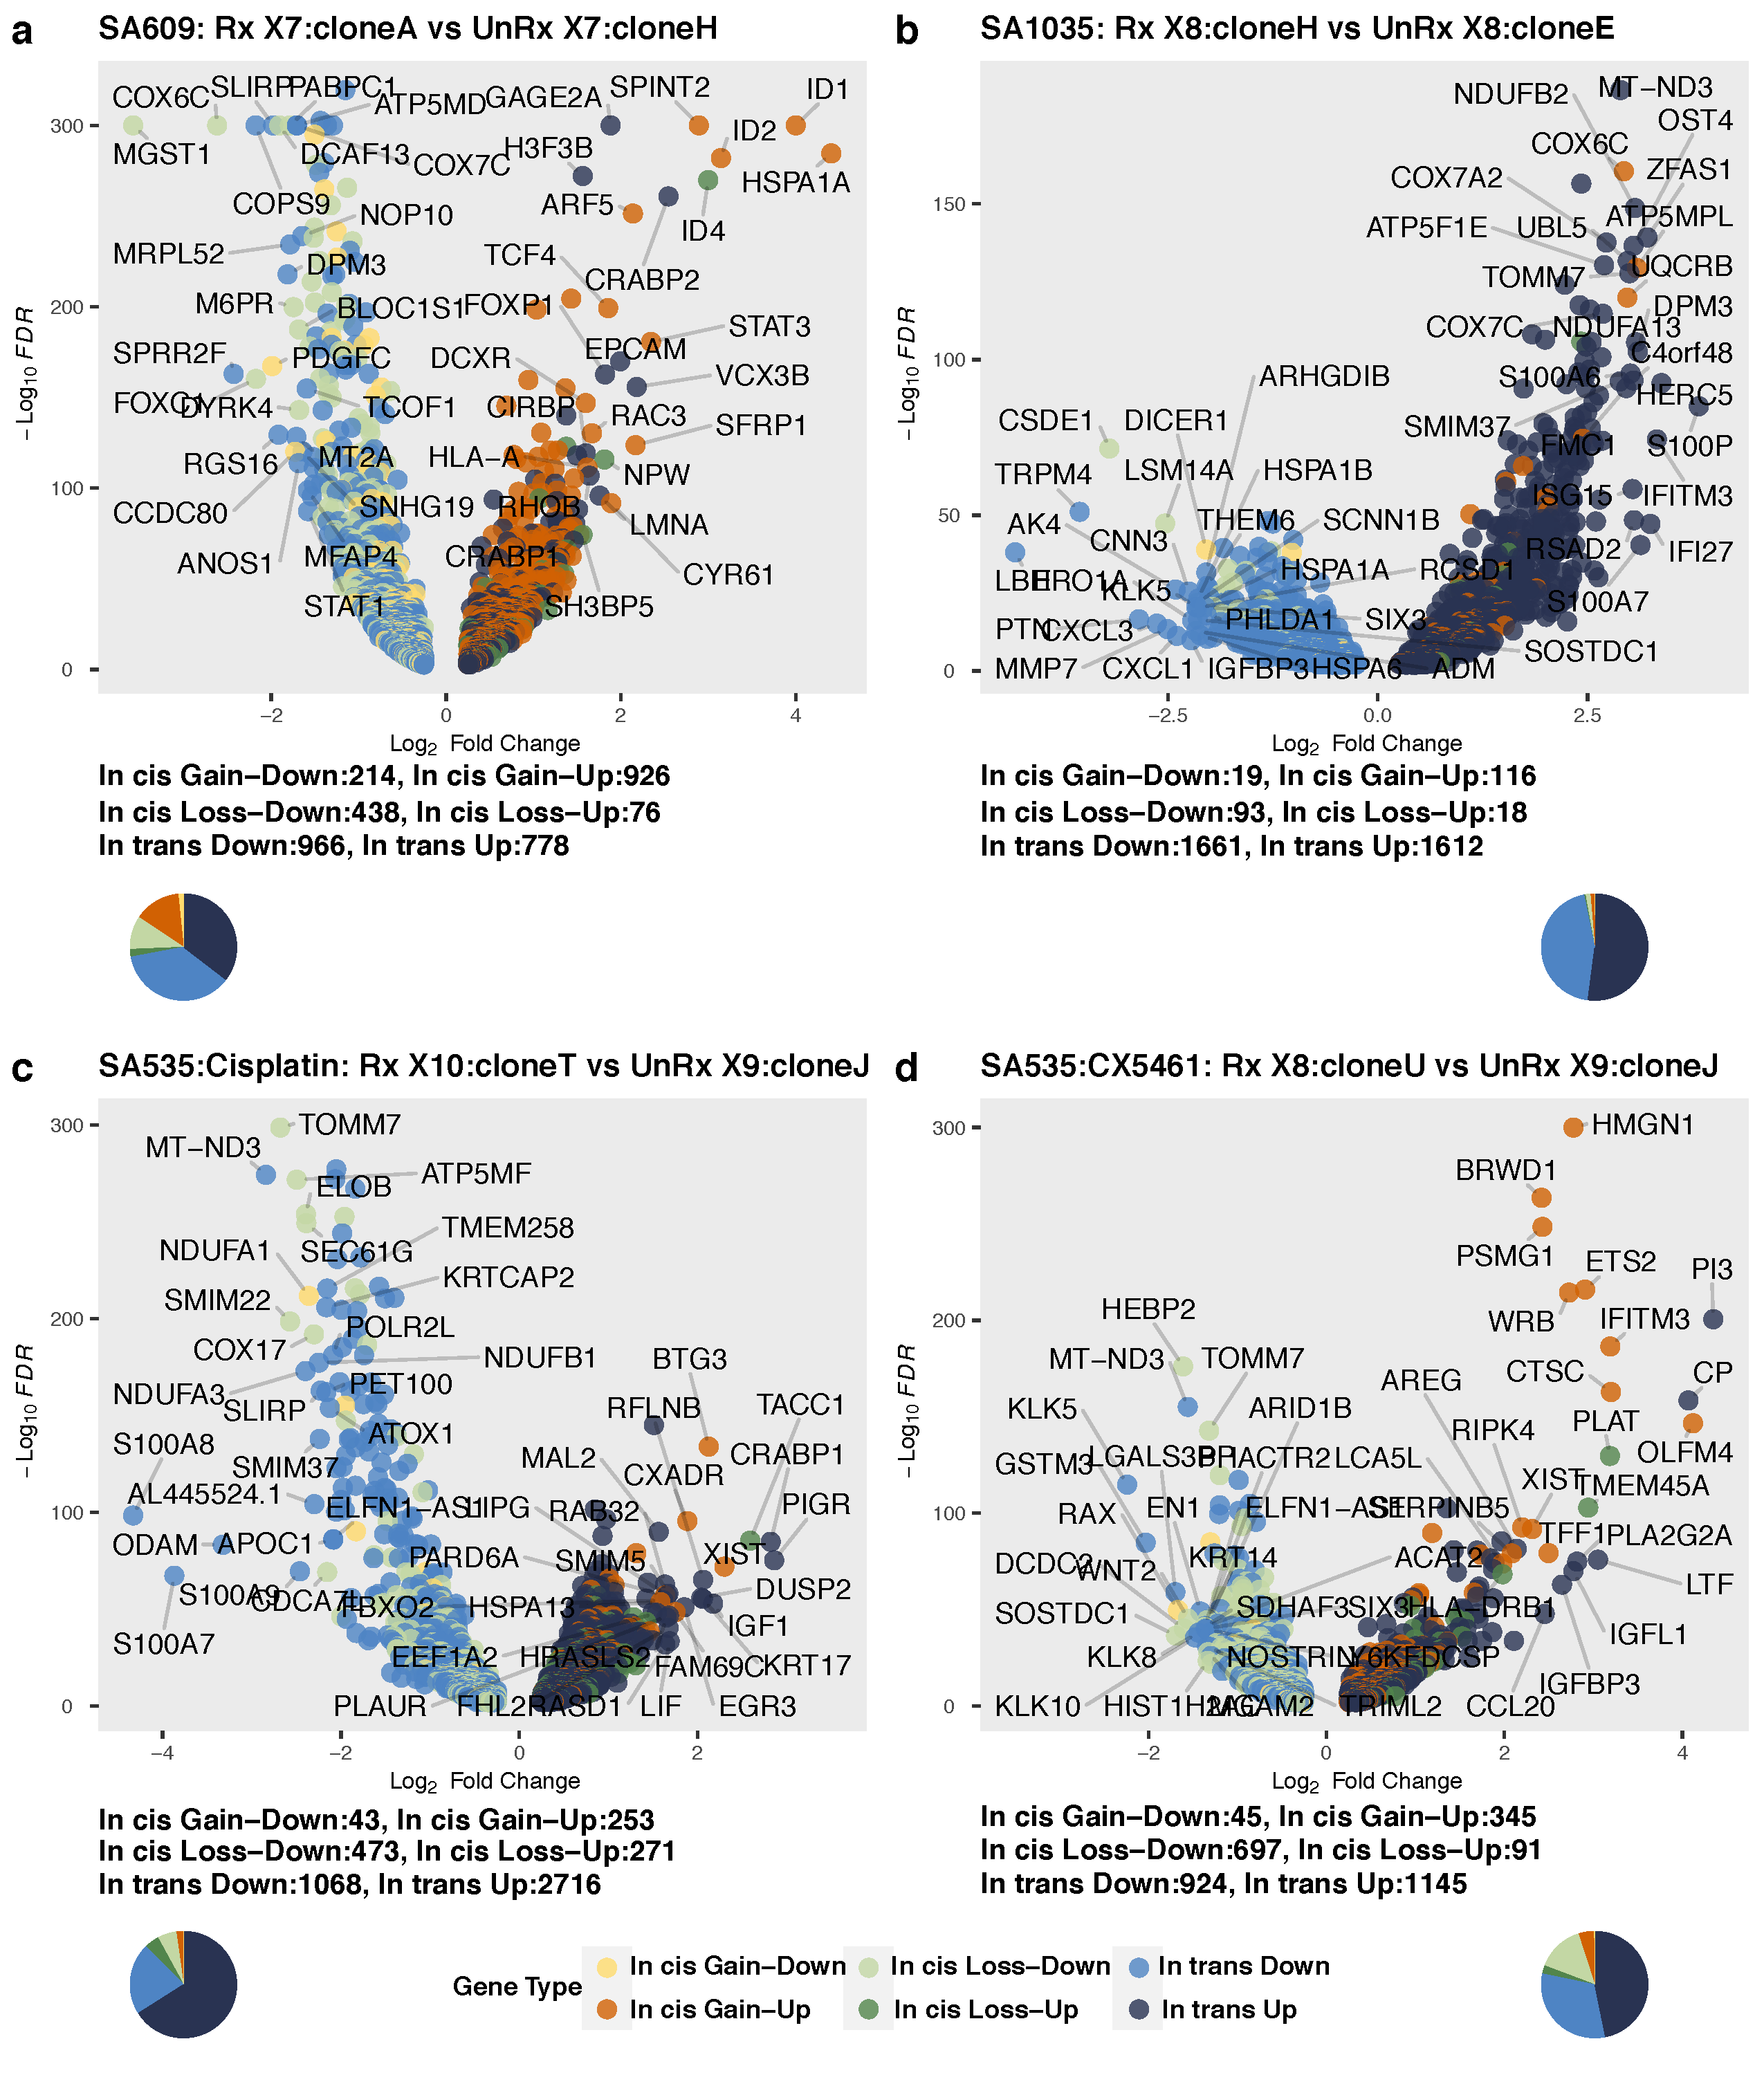
\includegraphics[width=\textwidth]{Figures/chap5/Volcanoes4plots.png}
\caption[DE of resistant and sensitive clonealign defined clones]
	{\small
	\textbf{Differential expression of resistant and sensitive clones.}
	\textbf{(a)} Volcano plot from SA609 -log10 (FDR) plotted against log2 fold change of pairwise differential gene expression between resistant and sensitive clones. (The threshold for significant genes are FDR p$<$00.01, P Value p$<$00.05, logFC p$>$0 0.25). Manhattan plot (genome-wide view) of differential gene expression between pairs of clones, R vs H corresponding to change in gene expression (Right).
	    \textbf{(b)} Same like \textbf{a} but in SA1035 and comparing between pairs of clones, H vs E. 
	     \textbf{(c)} Same like \textbf{a} but in SA535 (cisplatin) and comparing between pairs of clones, S\_T vs J.
	      \textbf{(d)} Same like \textbf{a} but in SA535 (CX-5461) and comparing between pairs of clones, U vs J.
	 
	   }
	\label{fig:Volcanoes4plots}
 \end{figure}

%------------------------------------------------------------

\begin{figure}
\centering
  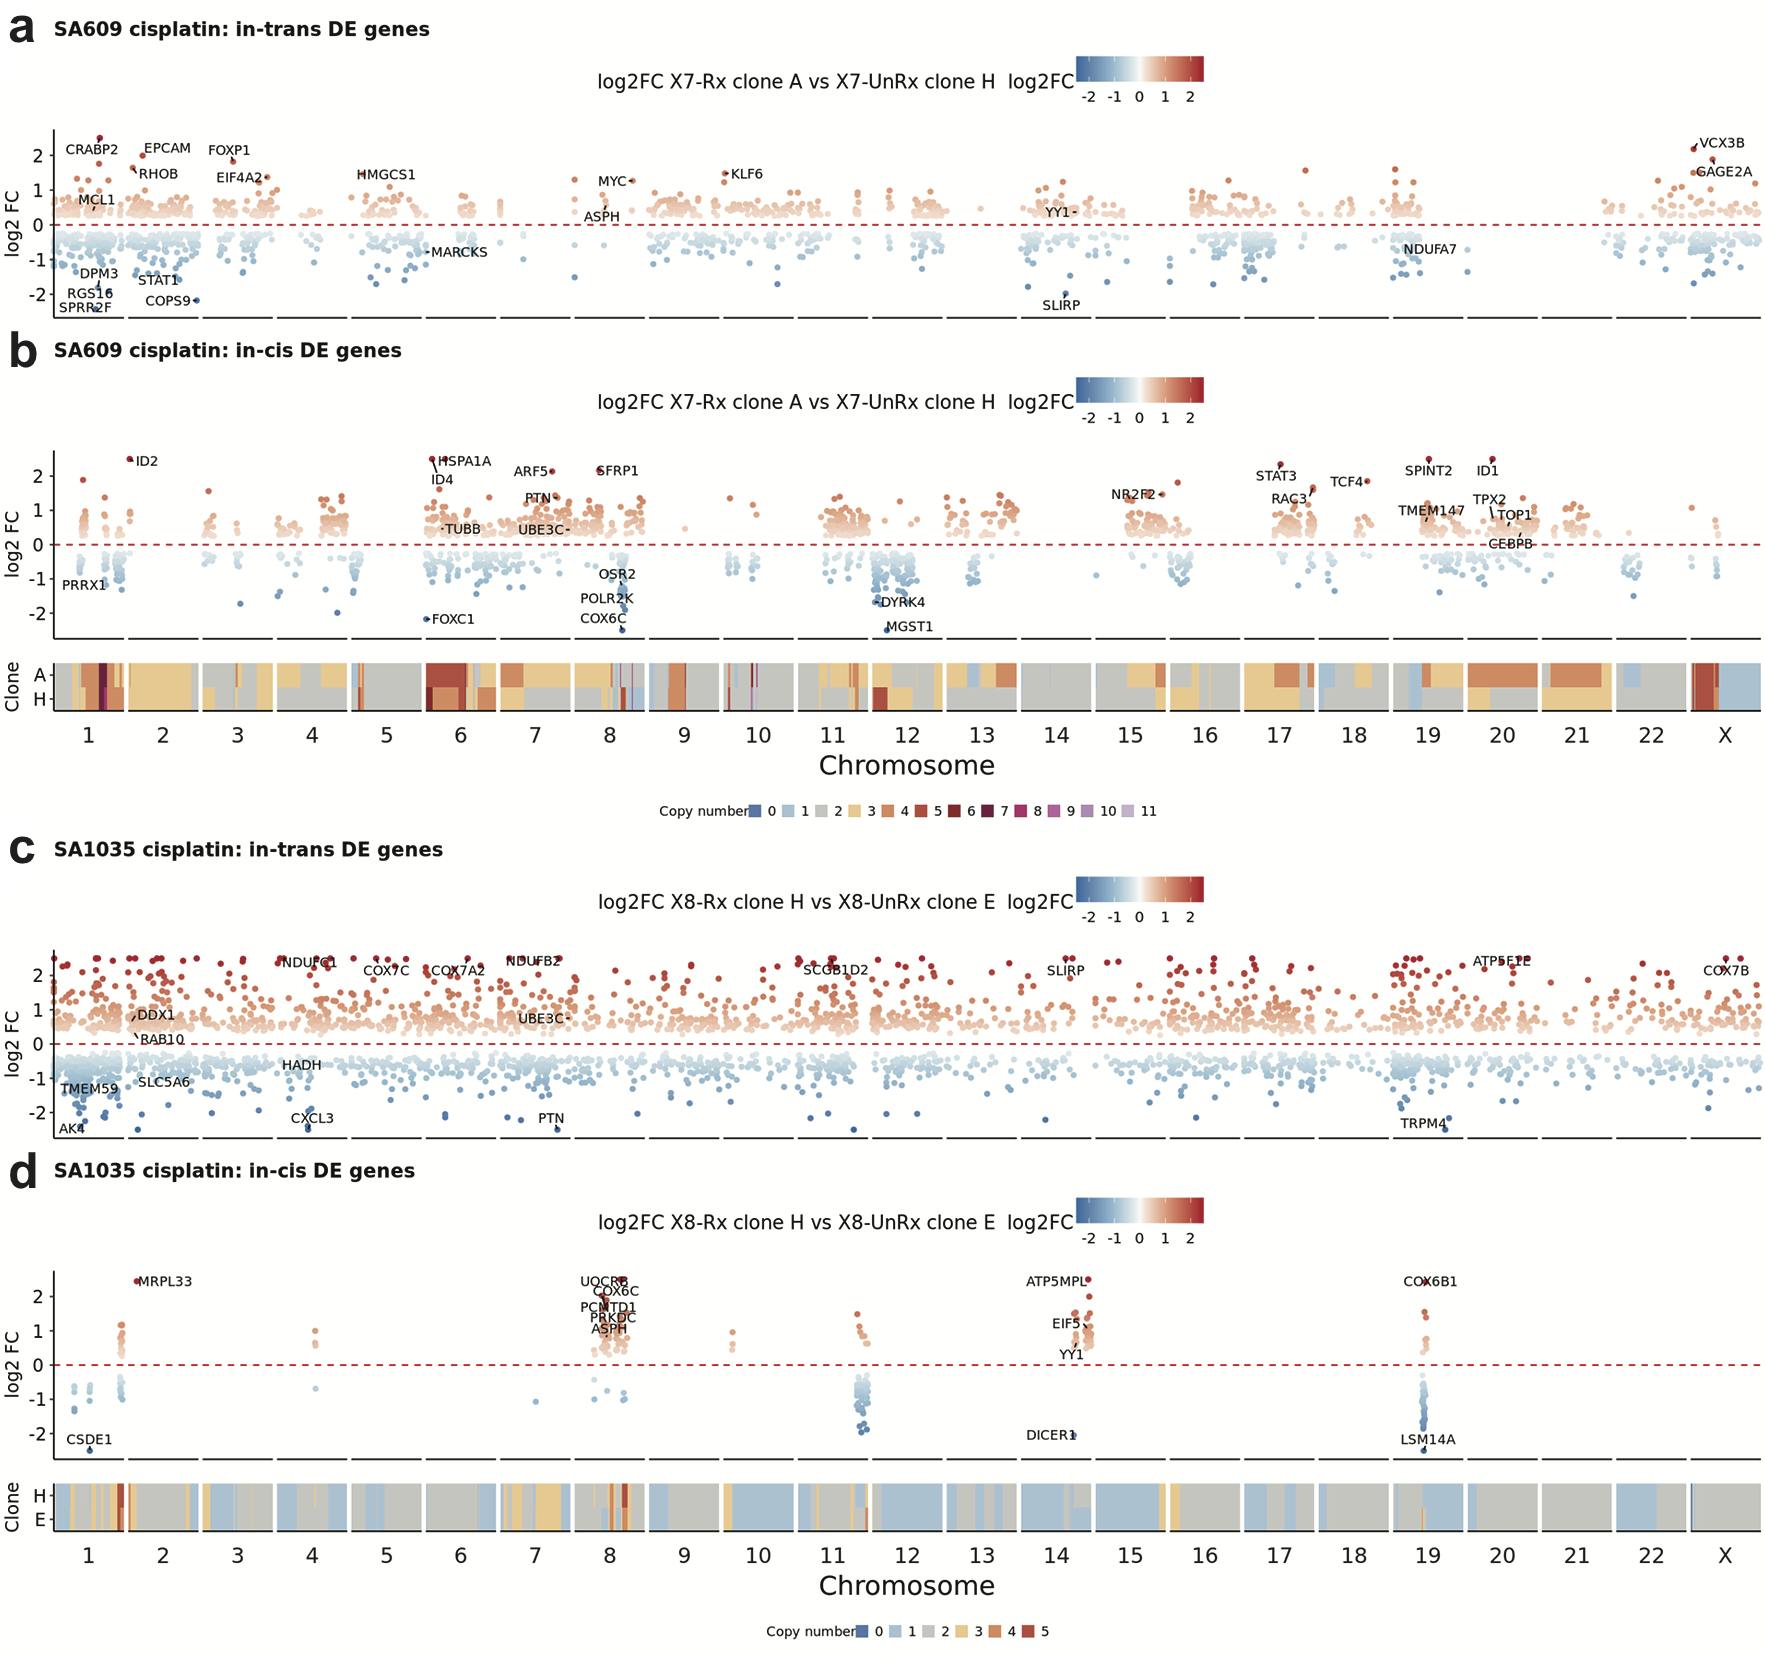
\includegraphics[width=\textwidth]{Figures/chap5/trackplotsSA609SA1035.png}
\caption[DE of resistant and sensitive clonealign defined clones]
	{\small
	\textbf{Differential expression of resistant and sensitive clones in TNBC-SA609 and TNBC-SA1035.}
 In each panel, the upper portion shows $\log 2$ fold change, with red showing higher log fold change in the top clone and blue showing higher log fold change in the bottom clone. The lower portion shows the median copy number of each gene from the DLP+ data, in the rank order of appearance in the genome.  Differential gene expression between the resistant and sensitive clone. The percentage of \textit{in-cis} differentially expressed genes (DEGs) is calculated as having a corresponding change in copy number, out of all the DEGs considered. 
 \textbf{(a)} Upper panel shows Manhattan plots of \textit{in cis} DEG, while bottom panel shows \textit{in trans} in TNBC-SA609.
 \textbf{(b)} Same as \textbf{(a)} but in TNBC-SA1035.
}
	\label{fig:trackplotsSA609SA1035}
 \end{figure}

%------------------------------------------------------------
\begin{figure}
\centering
  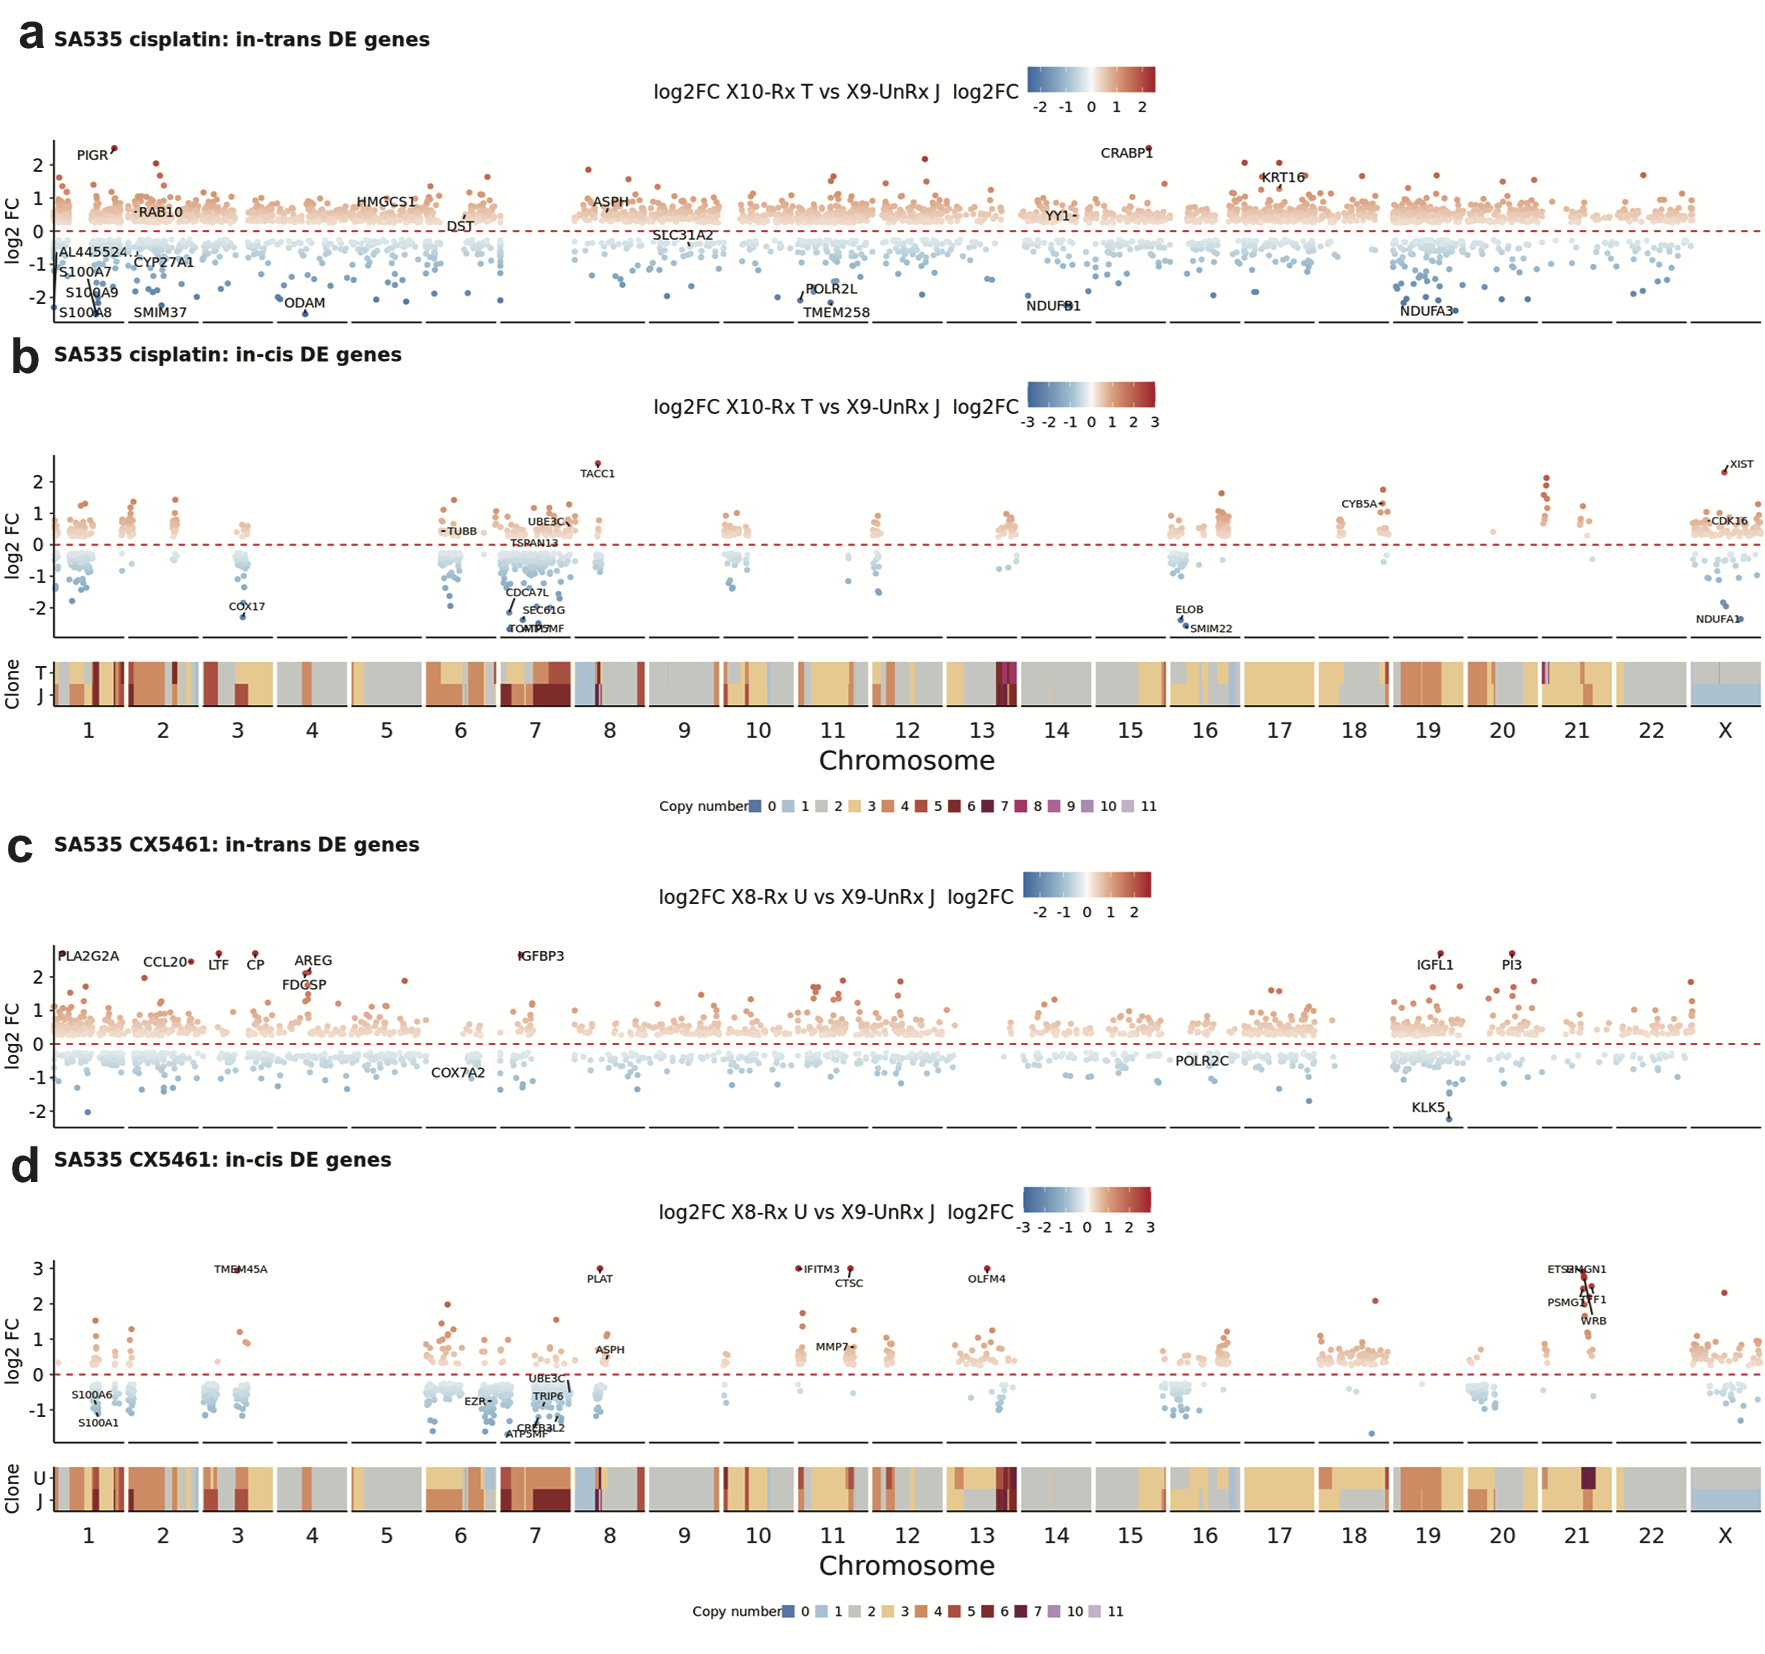
\includegraphics[width=\textwidth]{Figures/chap5/trackplotsSA535.png}
\caption[DE of resistant and sensitive clonealign defined clones]
	{\small
	\textbf{Differential expression of resistant and sensitive clones in TNBC-SA535 treated with cisplatin and CX-5461.}
 In each panel, the upper portion shows $\log 2$ fold change, with red showing higher log fold change in the top clone and blue showing higher log fold change in the bottom clone. The lower portion shows the median copy number of each gene from the DLP+ data, in the rank order of appearance in the genome.  Differential gene expression between the resistant and sensitive clone. The percentage of \textit{in-cis} differentially expressed genes (DEGs) is calculated as having a corresponding change in copy number, out of all the DEGs considered. 
 \textbf{(a)} Upper panel shows Manhattan plots of \textit{in cis} DEG, while bottom panel shows \textit{in trans} in TNBC-SA609.
 \textbf{(b)} Same as  \textbf{(a)} but in TNBC-SA1035.
}
	\label{fig:trackplotsSA535}
 \end{figure}
%------------------------------------------------------------

\begin{figure}
\centering
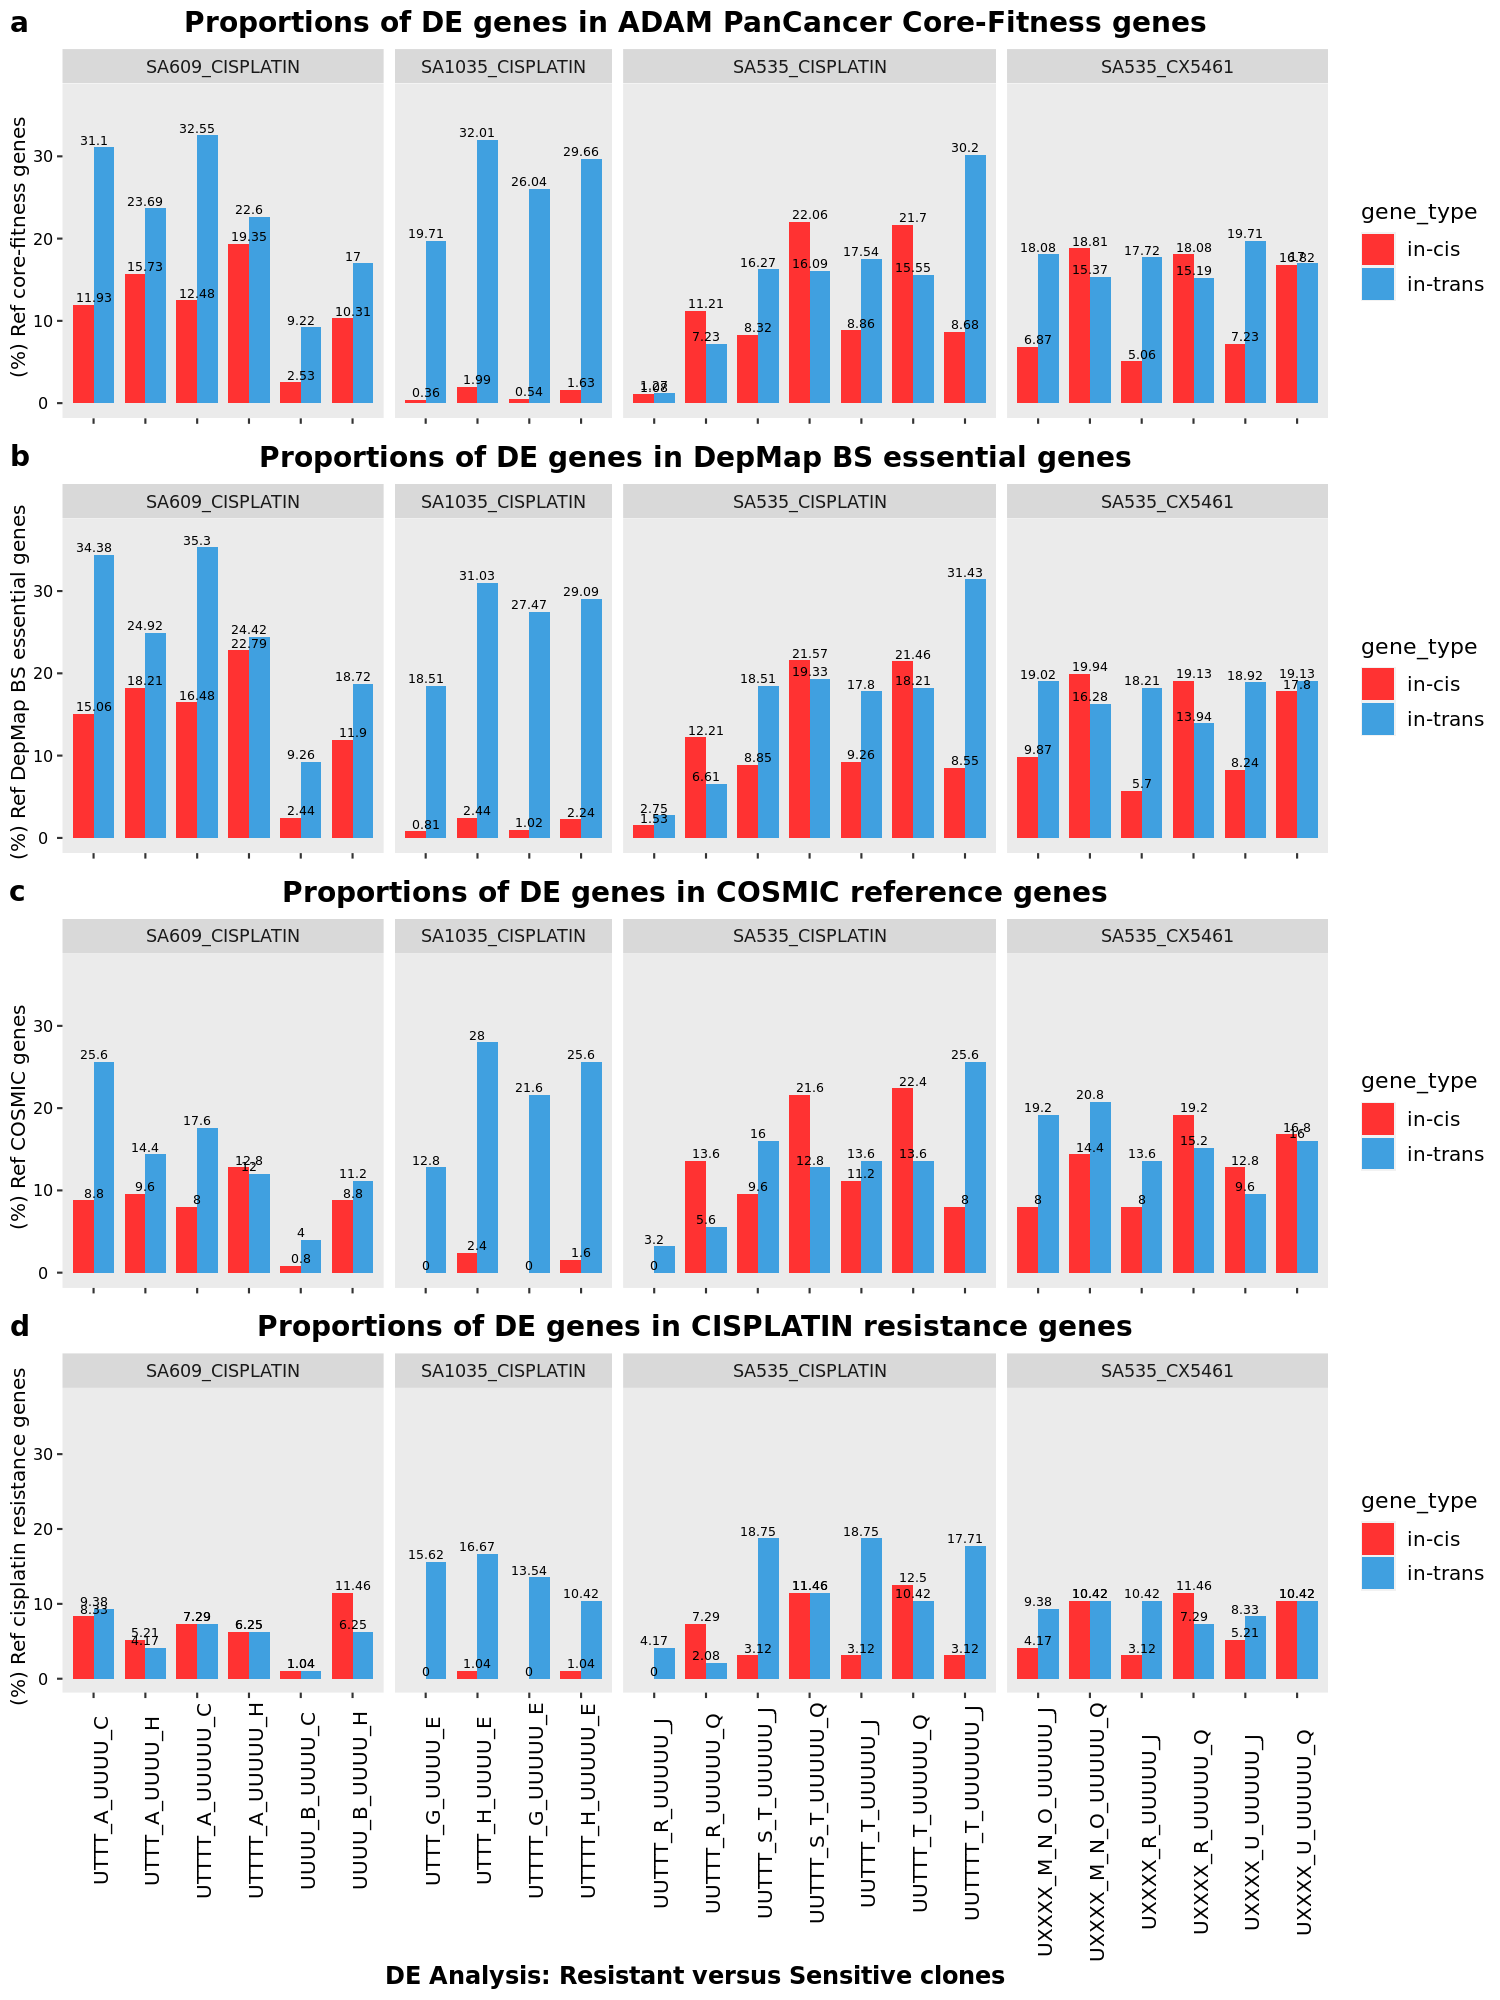
\includegraphics[width=\textwidth]{Figures/chap5/incispercenatgeindatasets.png}

\caption[Summary of number of cisplatin resistance genes \textit{in-cis} and \textit{in-trans}]
	{\small
	\textbf{Matching gene proportions in various datasets}

}
    \label{fig:incisgenesindatasets}
    \end{figure}


%------------------------------------------------------------------
\subsubsection{Differentially expressed genes in resistant clones showed positive match to cisplatin resistance genes}
%{Proportions of cisplatin resistance genes from various database}
Next, we probed various databases, including COSMIC \cite{vogelstein2013cancer}, core cancer fitness \cite{behan2019prioritization} and cisplatin related genes curated from  recent literature \textbf{\autoref{tab:Cisplatinrelatedgenes}}, and asked 
what proportion of genes exist \textit{in cis} or \textit{in trans} in our data set from these catalogues. 

First we pulled the reference genes from these databases that were intersecting with our \ac{DE} dataset and calculated if they are regulated with the change in copy number.

 In TNBC-SA609 PDX, the mean number of \textit{in cis} genes was 1173.8 (segment positions, $\sigma$ = 494 \textit{in cis} genes, max= 1640, min=215), TNBC-SA1035 presented with the lowest \textit{in cis} with
 mean value of 187.8 (segment positions, $\sigma$ = 51 \textit{in cis} genes, max=246, min=144). TNBC-SA535 in cisplatin timeseries showed mean number of 1056.9 \textit{in cis} genes (segment positions, $\sigma$ = 624 , max=1900, min=116), whereas, TNBC-SA535 in CX-5461 exhibit highest number of mean \textit{in cis} value of 1400.7 (segment positions, $\sigma$ = 481 \textit{in cis} genes, max=1884, min=739).
 
 Overall, our results remained consistent with the fact that the proportion of \textit{in trans} regulation of gene expression is higher than the \textit{in cis} in all the time series PDXs and from all the reference lists.   
 
 Interestingly, we noticed that TNBC-SA535 in both treatment regimes, inferred highest rate of \textit{in cis} genes with 28\% maximum, whereas, TNBC-SA1035 possessing the lowest rate of 2.4\% maximum. TNBC-SA609  showed 12.8\% of its highest \textit{in cis} gene rate \textbf{\autoref{fig:incisgenesindatasets}}.

%------------------------------------------------------------------

% Please add the following required packages to your document preamble:
% \usepackage{lscape}

\begin{landscape}
\begin{table}
\centering

 \caption{Summary of number of differentially expressed genes \textit{in cis} and \textit{in trans} in major clones}


\resizebox{\textwidth}{!}{%
\begin{tabular}{|l|p{3.8em}|p{3.8em}|p{3.8em}|p{3.8em}|p{3.8em}|p{3.8em}|}
\hline
DE scRNAseq between clones &
  In\_cis\_Decrease\_DownRegulated &
  In\_cis\_Decrease\_UpRegulated &
  In\_cis\_Increase\_DownRegulated &
  In\_cis\_Increase\_UpRegulated &
  In\_trans\_DownRegulated &
  In\_trans\_UpRegulated \\
  \hline
SA609-UUUU-B\_vs\_UUUU-C           & 79  & 44  & 40  & 52   & 399  & 382  \\
SA609-UUUU-B\_vs\_UUUU-H           & 127 & 186 & 471 & 636  & 1005 & 1207 \\
SA609-UTTT-A\_vs\_UUUU-C           & 655 & 150 & 48  & 425  & 1466 & 1817 \\
SA609-UTTT-A\_vs\_UUUU-H           & 352 & 69  & 177 & 611  & 850  & 659  \\
SA609-UTTTT-A\_vs\_UUUUU-C         & 603 & 174 & 43  & 461  & 1394 & 1894 \\
\textbf{*}SA609-UTTTT-A\_vs\_UUUUU-H         & 435 & 75  & 208 & 922  & 975  & 783  \\
SA1035-UTTTT-G\_vs\_UUUUU-E        & 55  & 7   & 11  & 71   & 1841 & 1125 \\
\textbf{*}SA1035-UTTTT-H\_vs\_UUUUU-E        & 93  & 18  & 19  & 116  & 1661 & 1612 \\
SA1035-UTTT-G\_vs\_UUUU-E          & 35  & 3   & 2   & 106  & 696  & 1368 \\
SA1035-UTTT-H\_vs\_UUUU-E          & 69  & 11  & 11  & 124  & 1004 & 2440 \\
\textbf{*}SA535\_UUTTTT-T\_vs\_UUUUUU-J      & 469 & 271 & 13  & 155  & 1102 & 2814 \\
SA535\_UUTTT-T\_vs\_UUUUU-J        & 599 & 97  & 6   & 128  & 791  & 1240 \\
SA535\_UUTTT-S\_T\_vs\_UUUUU-J     & 595 & 97  & 5   & 126  & 811  & 1235 \\
SA535-UUTTT-R\_vs\_UUUUU-J         & 38  & 12  & 7   & 59   & 177  & 188  \\
SA535\_UUTTT-T\_vs\_UUUUU-Q        & 831 & 183 & 57  & 765  & 681  & 1184 \\
SA535-UUTTT\_S\_T\_vs\_UUUUU-Q     & 834 & 200 & 54  & 812  & 696  & 1243 \\
SA535-UUTTT-R\_vs\_UUUUU-Q         & 294 & 80  & 33  & 578  & 365  & 483  \\
\textbf{*}SA535-UXXXX-U\_vs\_UUUUU-J & 697 & 91  & 21  & 286  & 948  & 1204 \\
SA535-UXXXX-U\_vs\_UUUUU-Q         & 695 & 167 & 61  & 820  & 771  & 1324 \\
SA535-UXXXX-R\_vs\_UUUUU-J         & 448 & 70  & 18  & 203  & 1178 & 1002 \\
SA535-UXXXX-R\_vs\_UUUUU-Q         & 646 & 130 & 70  & 1038 & 823  & 1063 \\
SA535\_UXXXX\_M\_N\_O\_vs\_UUUUU-J & 746 & 145 & 14  & 202  & 961  & 1307 \\
SA535-UXXXX-M\_N\_O\_vs\_UUUUU\_Q  & 753 & 296 & 48  & 739  & 710  & 1281 \\
  \hline

\end{tabular}
}

\label{tab:numberofDEgenesincistrans}

  \small\textbf{(* Resistant vs sensitive clones at the last time point of treatment cycle}.
\end{table}
\end{landscape}

%------------------------------------------------------------------

 
%------------------------------------------------------------------

% Table generated by Excel2LaTeX from sheet 'top20genes_incis upregulated in'
 \begin{table}[htbp]
   \centering
   \caption{Top 20 \textit{in cis} upregulated genes in TNBC-SA609 resistant clone vs sensitive}
     
     \begin{tabular}{|l|r|r|l|}
     \hline
     \textbf{Gene\_ID} & \multicolumn{1}{|l|}{ \textbf{Copy no. in A}}& \multicolumn{1}{|l|}{ \textbf{Copy no. in H}} &  \textbf{Gene\_regulation} \\
     \hline
     HSPA1A & 5 & 4 & In\_cis\_Increase\_UpRegulated \\
     ID1 & 4 & 2 & In\_cis\_Increase\_UpRegulated \\
     ID2 & 4 & 3 & In\_cis\_Increase\_UpRegulated \\
     ID4 & 5 & 6 & In\_cis\_Decrease\_UpRegulated \\
     SPINT2 & 4 & 2 & In\_cis\_Increase\_UpRegulated \\
     STAT3 & 4 & 3 & In\_cis\_Increase\_UpRegulated \\
     SFRP1 & 3 & 2 & In\_cis\_Increase\_UpRegulated \\
     ARF5 & 3 & 2 & In\_cis\_Increase\_UpRegulated \\
     CYR61 & 4 & 3 & In\_cis\_Increase\_UpRegulated \\
     TCF4 & 3 & 2 & In\_cis\_Increase\_UpRegulated \\
     NPW & 2 & 3 & In\_cis\_Decrease\_UpRegulated \\
     RAC3 & 4 & 2 & In\_cis\_Increase\_UpRegulated \\
     HLA-A & 5 & 4 & In\_cis\_Increase\_UpRegulated \\
     DCXR & 4 & 2 & In\_cis\_Increase\_UpRegulated \\
     SH3BP5 & 2 & 3 & In\_cis\_Decrease\_UpRegulated \\
     CRABP1 & 3 & 2 & In\_cis\_Increase\_UpRegulated \\
     NR2F2 & 4 & 3 & In\_cis\_Increase\_UpRegulated \\
     DNAJC3 & 4 & 2 & In\_cis\_Increase\_UpRegulated \\
     MEST & 3 & 2 & In\_cis\_Increase\_UpRegulated \\
     RCN2 & 3 & 2 & In\_cis\_Increase\_UpRegulated \\
     
    \hline
     \end{tabular}%
  
   \label{tab:top20SA609upregulated}%
   
    \small\textbf{(** (FDR$<$0.01, p$<$0.05))}.
 \end{table}%

%------------------------------------------------------------------
 % Table generated by Excel2LaTeX from sheet 'Sheet1'
 \begin{table}[htbp]
   \centering
   \caption{Top 20 upregulated \textit{in cis} genes in TNBC-SA1035 resistant clone vs sensitive}
     \begin{tabular}{|l|r|r|l|r}
     \hline
     \textbf{Gene\_ID} & \multicolumn{1}{|l|}{\textbf{Copy no. in H}} & \multicolumn{1}{|l|}{\textbf{Copy no. in E}} & \textbf{Gene regulation**}\\
     
     \hline
     ATP5MPL & 2 & 1 & In\_cis\_Increase\_UpRegulated \\
     UQCRB & 2 & 1 & In\_cis\_Increase\_UpRegulated   \\
     COX6C & 5 & 3 & In\_cis\_Increase\_UpRegulated  \\
     MRPL33 & 3 & 2 & In\_cis\_Increase\_UpRegulated \\
     COX6B1 & 1 & 2 & In\_cis\_Decrease\_UpRegulated  \\
     PRKDC & 2 & 1 & In\_cis\_Increase\_UpRegulated  \\
     PCMTD1 & 2 & 1 & In\_cis\_Increase\_UpRegulated \\
     SIVA1 & 2 & 1 & In\_cis\_Increase\_UpRegulated \\
     YTHDF3-AS1 & 2 & 1 & In\_cis\_Increase\_UpRegulated \\
     RAB2A & 2 & 1 & In\_cis\_Increase\_UpRegulated \\
     TCEA1 & 2 & 1 & In\_cis\_Increase\_UpRegulated  \\
     FXYD3 & 1 & 2 & In\_cis\_Decrease\_UpRegulated  \\
     BCL11B & 2 & 1 & In\_cis\_Increase\_UpRegulated  \\
     ENY2 & 5 & 4 & In\_cis\_Increase\_UpRegulated  \\
     AHNAK2 & 2 & 1 & In\_cis\_Increase\_UpRegulated  \\
     CLMN & 2 & 1 & In\_cis\_Increase\_UpRegulated  \\
     TIMM8B & 1 & 2 & In\_cis\_Decrease\_UpRegulated  \\
     PLEKHF2 & 2 & 1 & In\_cis\_Increase\_UpRegulated  \\
     PSENEN & 1 & 2 & In\_cis\_Decrease\_UpRegulated  \\
     CKB & 2 & 1 & In\_cis\_Increase\_UpRegulated  \\
     
     \hline
     \end{tabular}%
   
   \label{tab:top20SA1035upregulated}%
 
   \small\textbf{(** (FDR$<$0.01, p$<$0.05))}.
 \end{table}%

%-----------------------------------------------------------------

 % Table generated by Excel2LaTeX from sheet 'Sheet1'
 \begin{table}[htbp]
   \centering
   \caption{Top 20 upregulated \textit{in cis} genes in SA535-TNBC cisplatin resistant clone vs sensitive}
     \begin{tabular}{|l|r|r|l|}
     \hline
     \textbf{Gene\_ID} & \multicolumn{1}{|l|}{\textbf{Copy no. in T}} & \multicolumn{1}{|l|}{\textbf{Copy no. in J}} & \textbf{Gene regulation**} \\
     \hline
     TACC1 & 6 & 7 & In\_cis\_Decrease\_UpRegulated \\
     XIST & 2 & 1 & In\_cis\_Increase\_UpRegulated \\
     BTG3 & 11 & 3 & In\_cis\_Increase\_UpRegulated \\
     CXADR & 11 & 3 & In\_cis\_Increase\_UpRegulated \\
     FAM69C & 3 & 2 & In\_cis\_Increase\_UpRegulated \\
     PARD6A & 3 & 2 & In\_cis\_Increase\_UpRegulated \\
     HSPA13 & 8 & 3 & In\_cis\_Increase\_UpRegulated \\
     C21orf91 & 11 & 3 & In\_cis\_Increase\_UpRegulated \\
     CHN1 & 6 & 4 & In\_cis\_Increase\_UpRegulated \\
     PIM1 & 3 & 4 & In\_cis\_Decrease\_UpRegulated \\
     FKBP1B & 5 & 6 & In\_cis\_Decrease\_UpRegulated \\
     CYB5A & 3 & 2 & In\_cis\_Increase\_UpRegulated \\
     F3 & 2 & 3 & In\_cis\_Decrease\_UpRegulated \\
     FLNA & 2 & 1 & In\_cis\_Increase\_UpRegulated \\
     INSIG1 & 5 & 6 & In\_cis\_Decrease\_UpRegulated \\
     GADD45A & 3 & 4 & In\_cis\_Decrease\_UpRegulated \\
     ETS2 & 4 & 3 & In\_cis\_Increase\_UpRegulated \\
     RRM2 & 5 & 6 & In\_cis\_Decrease\_UpRegulated \\
     CAV1 & 5 & 6 & In\_cis\_Decrease\_UpRegulated \\
     CDK14 & 4 & 6 & In\_cis\_Decrease\_UpRegulated \\
     \hline
     \end{tabular}%
   \label{tab:top20SA535upregulatedcispl}%
 
   \small\textbf{(** (FDR$<$0.01, p$<$0.05))}.
 \end{table}%


%-------------------------------------------------------------------
 % Table generated by Excel2LaTeX from sheet 'Sheet1'
 \begin{table}[htbp]
   \centering
   \caption{Top 20 upregulated \textit{in cis} genes in TNBC-SA535-TNBC  resistant clone vs sensitive}
     \begin{tabular}{|l|r|r|l|}
     \hline
     \textbf{Gene\_ID} & \multicolumn{1}{|l|}{\textbf{Copy no. in  U} }& \multicolumn{1}{|l|}{\textbf{Copy no. in  J}} & \textbf{Gene regulation**} \\
     \hline
     OLFM4 & 3 & 2 & In\_cis\_Increase\_UpRegulated \\
     CTSC & 5 & 4 & In\_cis\_Increase\_UpRegulated \\
     IFITM3 & 5 & 4 & In\_cis\_Increase\_UpRegulated \\
     PLAT & 7 & 11 & In\_cis\_Decrease\_UpRegulated \\
     TMEM45A & 4 & 5 & In\_cis\_Decrease\_UpRegulated \\
     ETS2 & 7 & 3 & In\_cis\_Increase\_UpRegulated \\
     HMGN1 & 7 & 4 & In\_cis\_Increase\_UpRegulated \\
     WRB & 7 & 4 & In\_cis\_Increase\_UpRegulated \\
     TFF1 & 7 & 4 & In\_cis\_Increase\_UpRegulated \\
     PSMG1 & 7 & 4 & In\_cis\_Increase\_UpRegulated \\
     BRWD1 & 7 & 4 & In\_cis\_Increase\_UpRegulated \\
     XIST & 2 & 1 & In\_cis\_Increase\_UpRegulated \\
     RIPK4 & 7 & 4 & In\_cis\_Increase\_UpRegulated \\
     SERPINB5 & 3 & 2 & In\_cis\_Increase\_UpRegulated \\
     HLA-DRB1 & 3 & 4 & In\_cis\_Decrease\_UpRegulated \\
     LCA5L & 7 & 4 & In\_cis\_Increase\_UpRegulated \\
     PHLDA2 & 5 & 4 & In\_cis\_Increase\_UpRegulated \\
     SH3BGR & 7 & 4 & In\_cis\_Increase\_UpRegulated \\
     AKR1B1 & 4 & 6 & In\_cis\_Decrease\_UpRegulated \\
     IVL & 5 & 6 & In\_cis\_Decrease\_UpRegulated \\
     \hline
     \end{tabular}%
   \label{tab:top20SA535upregulatedCX}%
 
  \small\textbf{(** (FDR$<$0.01, p$<$0.05))}.

 \end{table}%






%--------------------------------------------------------------------

In \textbf{SA535} TNBC PDX, both timeseries from two different drugs showed up with somewhat distinct set of regulated genes. Interestingly, the first upregulated gene, \textit{(incis\_IU)}, that caught our attention was on chromosome X, \textit{\textbf{XIST}} \cite{salama2020xist,chen2017long, chen2019up}, in both independently treated different drug series. 
In addition, other \textbf{cisplatin} related set of genes in this PDX comprised of \textit{\textbf{TACC1}}, which is upregulated \textit{(incis\_IU)} on chromosome 8, known to be amplified in 10-15\% of human breast cancers and plays a role in interactions between centrosomes and microtubules \cite{ray2004genomic, gergely2000tacc, shakya2018high},
 \textit{\textbf{COX17}}, downregulated in or resistant clone, is a human copper chaperone, that binds cisplatin \cite{katano2002acquisition, zhao2014cisplatin}, \textit{\textbf{CYP27A1} }is more specific in hapatocellular carcinoma but also seem to be expressed in high grade breast tumors \cite{liang2019cyp27a1, wu201327}, \textit{\textbf{SLC31A2}}, are membrane transporters known to be downregulated in resistance \cite{bai2017structural}. Other significant genes that could be under consideration for further validations in our cisplatin related data sets were \textit{\textbf{DST} } \cite{salerno2016human,lee2012differentially}, \textit{\textbf{HMGCS1}} \cite{walsh2020mevalonate},
\textit{\textbf{TAGLN}} \cite{wu2014transgelin, elsafadi2020transgelin},
\textit{\textbf{KRT16}} \cite{huang2019novel},
\textit{\textbf{IFITM3}} \cite{liu2019ifitm3} and
\textit{\textbf{S100A7}} \cite{zhang2019clinical, mayama2018olfm}. The top 20 upregulated genes with change in copy number are enlisted in \textbf{\autoref{tab:top20SA535upregulatedcispl}}.


% Please add the following required packages to your document preamble:
% \usepackage{graphicx}
\begin{table}[]
\caption{Upregulated common genes in resistant clones of all TNBC PDX}
\resizebox{0.55\textwidth}{!}{
\begin{tabular}{lllll}
\hline
PW             & APKAPK5-AS1    & CCDC28B \\
PPDPF            & CKB          & NCKAP1 \\
FARP1          & MAP3K2      & RAB10 \\
ZFHX3          & **YY1           & RYBP   \\
DRAP1         & C1orf56       & CPNE3   \\
NR4A1           & **UBE2H         & REX1BD \\
EIF1           & SUCO         & SCARB2  \\
TCAF1          & LYPLA1        & RAP2B  \\
CDKN2A        & NME1          & RRP1B   \\
FGFR1OP2      & POLR1D       & NOTCH2   \\
PITX1         & SS18L2        & CFAP36  \\
TNNT1           & ATXN2L       & RCAN1  \\
EIF3K           & TMEM68      & CENPK   \\
NUP58          & HSP90AA1      & CKS1B      \\
DLL3            & **UBE3C          & SREBF2    \\
SDCBP          & ANKLE2         & JPX   \\
SIVA1         & TATDN1          & TMEM189    \\
AP002387.2    & C9orf3       & CCDC107   \\
PSMA7         & DYNC1H1       & LARP6    \\
TCEA2         & EPB41        & UBXN2A     \\
MBOAT2        & RWDD4           & TFRC   \\
WASF2         & KIAA0232        & S100A10     \\
ZNF331          & CCSER2       & B4GALT5 \\
**ASPH         & GSTP1       & MRPL15  \\
ING2           & MRPL11          & PAXX           \\
ATP5PO         & APRT            &                  \\
      
\hline
\end{tabular}%
}
\label{tab:UpregulatedgenesinalltreatedPDX}

   \small\textbf{(**Genes randomly selected to check time dependent trajectories in 4 PDX  \textbf{\autoref{fig:commongenesfromvolcanoplots}}}.
   
\end{table}

%------------------------------------------------------------------------

In \textbf{SA535} treated with \textbf{CX-5461}, the differential expression of resistant and sensitive clones also resulted in known cancers related genes but potential candidates to explore further in relation to CX-5461 resistance related mechanisms. Top 20 upregulated genes are summarized with change in copy number in resistant and sensitive clones in \textbf{\autoref{tab:top20SA535upregulatedCX}}.
Highlighting some  includes \textbf{MMP7}, which is correlated with cancer invasion, metastasis, and poor prognosis \cite{mcgowan2008matrix} ,
\textit{\textbf{TMEM45A}}, known to cause chemoresistance in breast cancer \cite{schmit2019characterization},
\textit{\textbf{ETS2}}, functions as an oncogene and plays a key role in the progression of hypopharyngeal cancer and associated with poor prognosis \cite{fu2017high, ge2008role}.
\textit{\textbf{COX7A2}} is downregulated in resistant clone which is negatively correlated with prognosis \cite{deng2018overexpression},
\textit{\textbf{POLR2C}} mutation is known to progress ovarian cancers and its found downregulated in our resistant clone \cite {moriwaki2017polr2c} and
\textit{\textbf{OLFM4}} is reported to be highly expressed in cancers, including gastric cancer, colon cancer, and pancreatic cancer and to promote tumor progression by inducing cell cycle progression and enhancing tumor invasion and metastasis \cite{ashizawa2019olfm4}.


\subsubsection{Trend of common genes in all four TNBC PDX with  chemotherapy}
Next, we asked whether there is drug induced adaptive expression of common genes that could be seen in all timeseries. 
 Few genes were enlisted that were found to be increasing monotonically in all 4 TNBC PDX series. We recorded their expression at each time under various experimental conditions in all timeseries. Some of common genes were  \textit{\textbf{ASPH, CDKN2, RAB10, RCAN1, SCARB2, PAPOLA, UBE3C and YY1}}. The representative line trajectories from \textit{\textbf{ASPH}}, which is known to be upregulated in breast carcinoma, hepatic carcinoma, cervical cancer and ovarian cancer and contributes to enhancing cell migration  \cite{zheng2020diverse,li2018expression, hou2018recent, lin2019asph}, tend to rise under the drug in all series but less significantly in SA535 treated with cisplatin \textbf{\autoref{fig:commongenesfromvolcanoplots} a}. 
 \textit{\textbf{RAB10, (Member RAS Oncogene Family)}} is also found to be increasing monotonically with each cycle of drug in all 4 TNBC PDX \textbf{\autoref{fig:commongenesfromvolcanoplots} b}. It has been recently demonstrated to be aberrantly expressed in some of the cancers and show biological significance in tumor progression and prognosis, especially, in hepatocellular carcinoma \cite{wang2017rab10, he2002identification, jiang2016mir}. 
Another gene,  \textit{\textbf{UBE3C}} also seem to establish high expression in all 4 PDXs but more significantly in SA609 and SA535, treated with cisplatin \textbf{\autoref{fig:commongenesfromvolcanoplots} c}. The role of aberrant expression of ubiquitin protein ligase E3C (UBE3C) has not been widely studied in triple negative breast cancers but in ovarian cancer, gastric cancer, renal cell carcinoma and melanoma, it is known to promote proliferation and invasion and inhibition of apoptosis by activating the $\beta$-catenin signaling possibly via degradation of  \textit{AXIN1} \cite{xiong2019mir, pan2015ubiquitin, zhang2020ube3c}.
  Zinc-finger protein  \textit{\textbf{Yin Yang 1 (YY1)}}, In our data, YY1 expression remained high under the drug as compare to most of untreated timepoints \textbf{\autoref{fig:commongenesfromvolcanoplots} c}. YY1 generally over expressed in breast cancer cells 
is uniformly highly over-expressed in a wide range of human cancers including human colon cancer tissue samples. It involves numerous genes involved in cell proliferation, cell cycle, survival and cellular metabolism.  \cite{wan2012yin, chinnappan2009transcription, meliala2020biological}. Literature indicates that YY1 possesses a great potential as a biomarker for many cancers and can serve as a therapeutic target to impede cancer progression or sensitize cancer cells to chemotherapies \cite{wan2012yin, chinnappan2009transcription, meliala2020biological, shi2015role}.

%---------------------------------------------------------------------

%------------------------------------------------------------
 %\begin{figure}
%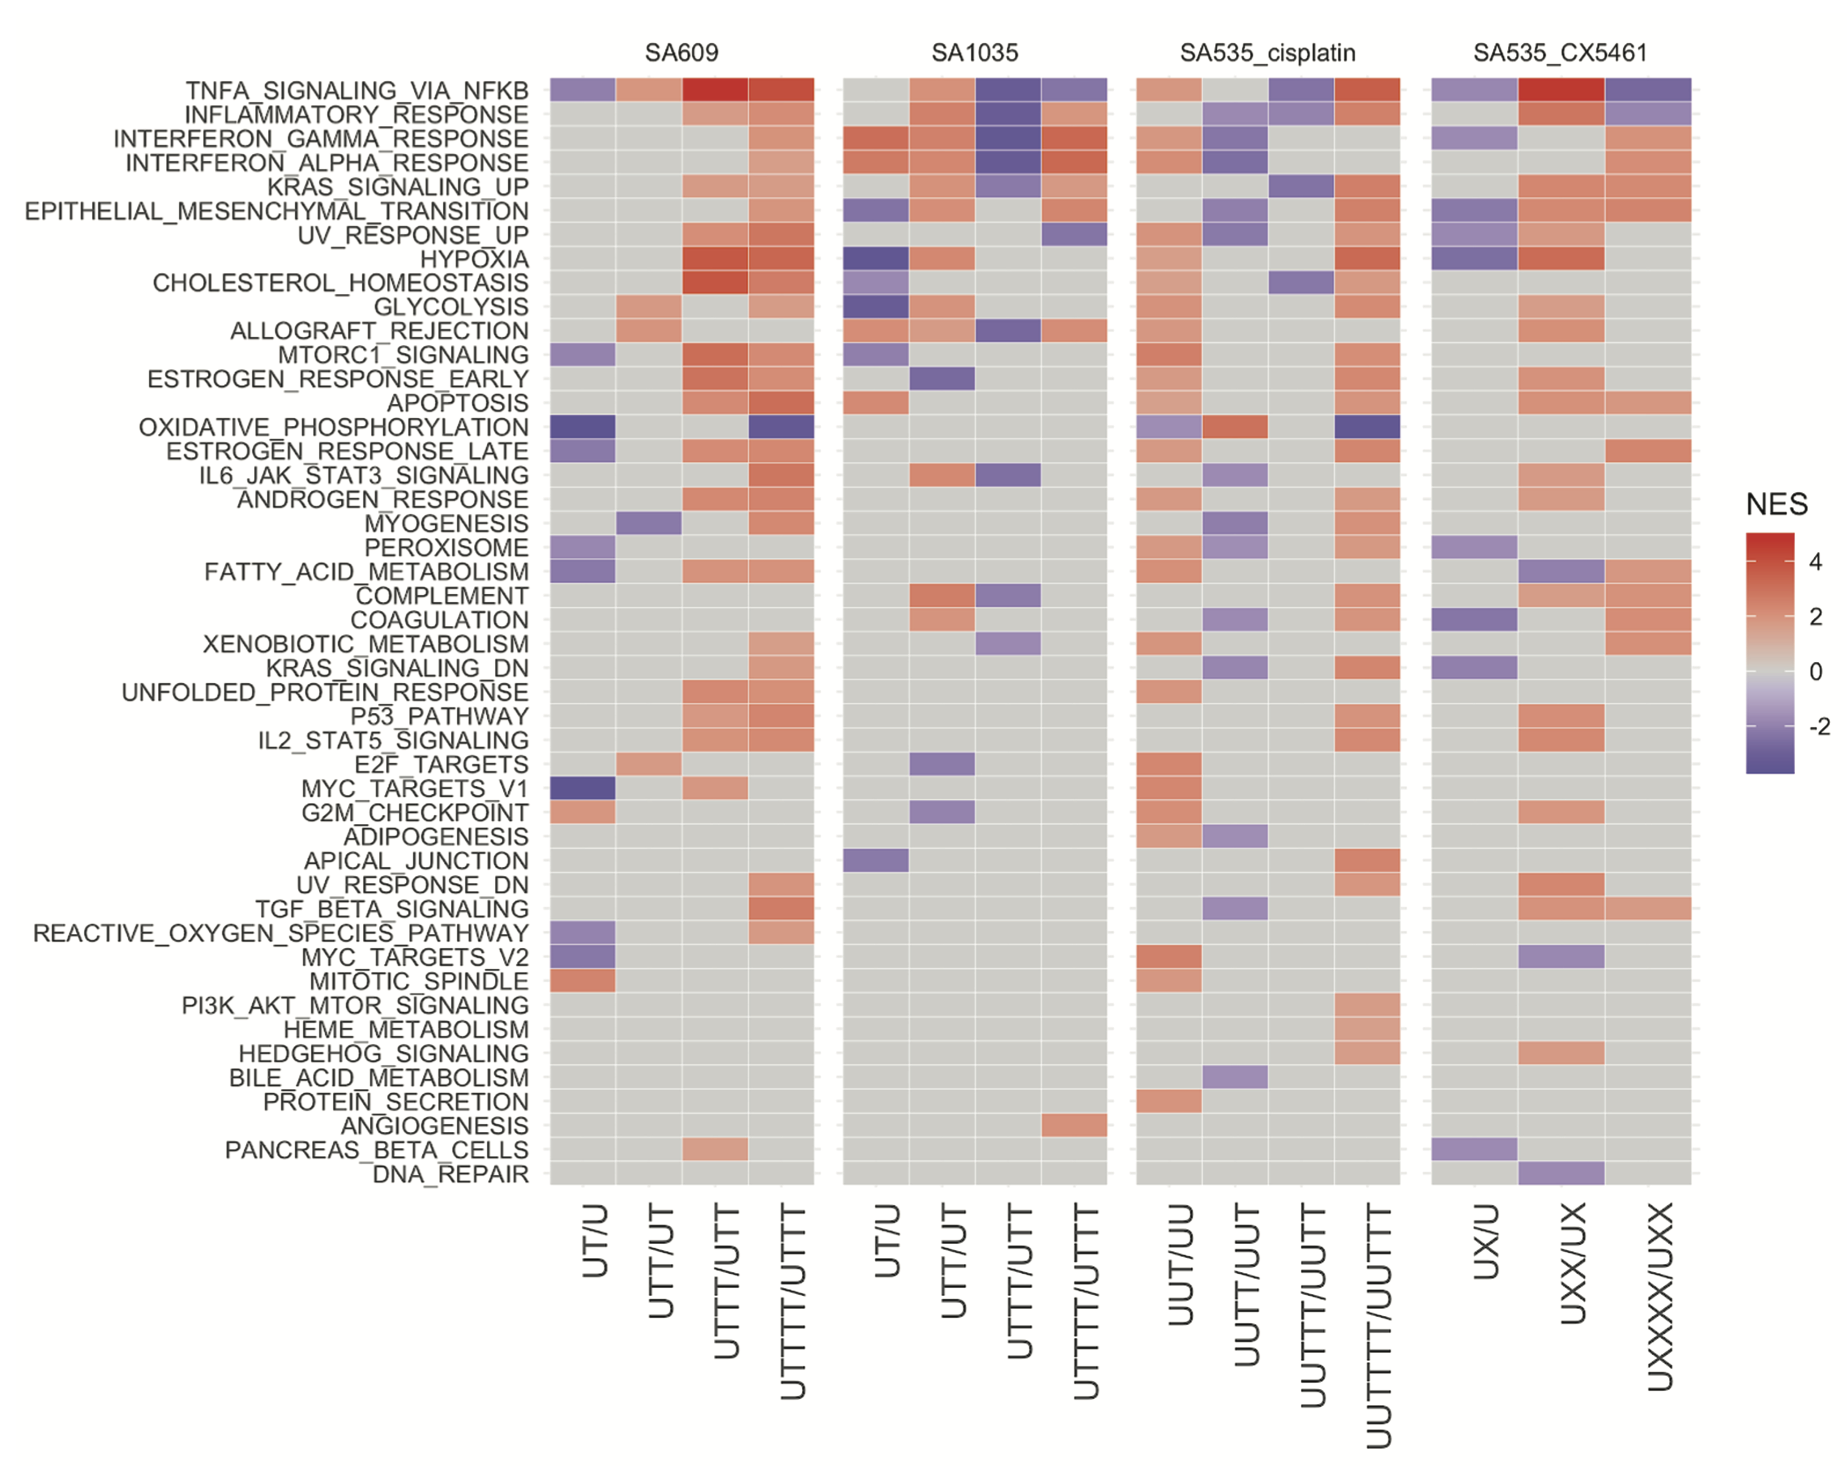
\includegraphics[width=\textwidth]{Figures/chap5/pathwaysevolution.png}
%\caption[Summary of number of genes \textit{in-cis} and \textit{in-trans}]
%	{\small
%	\textbf{Pathways comparison over time under chemotherapy in all PDX series}
%	Vertical left column enlist the pathways analysed. Horizontal axis at the bottom, represents the comparisons made between the time points and the treatment status. each single `T' indicates the number of cycles of the treatment from cisplatin. Each `X' indicates number of cycles of CX-5461 treatment. Colour intensity identifies normalized enrichment score (NES). Horizontal axis on top denotes the IDs of TNBC PDX. A normalized enrichment score (NES) was calculated from a ranked gene set enrichment analysis (GSEA) \cite{shi2007gene} performed on each subset of differentially expressed genes using the hallmark gene set collection from MSigDB \cite{liberzon2015molecular}.  Significantly enriched pathways (adjusted p-value $<$ 0.01).
%}
 %   \label{fig:pathwaysevolution}
%    \end{figure}
%-------------------------------------------------------------------
\begin{figure}
\centering
  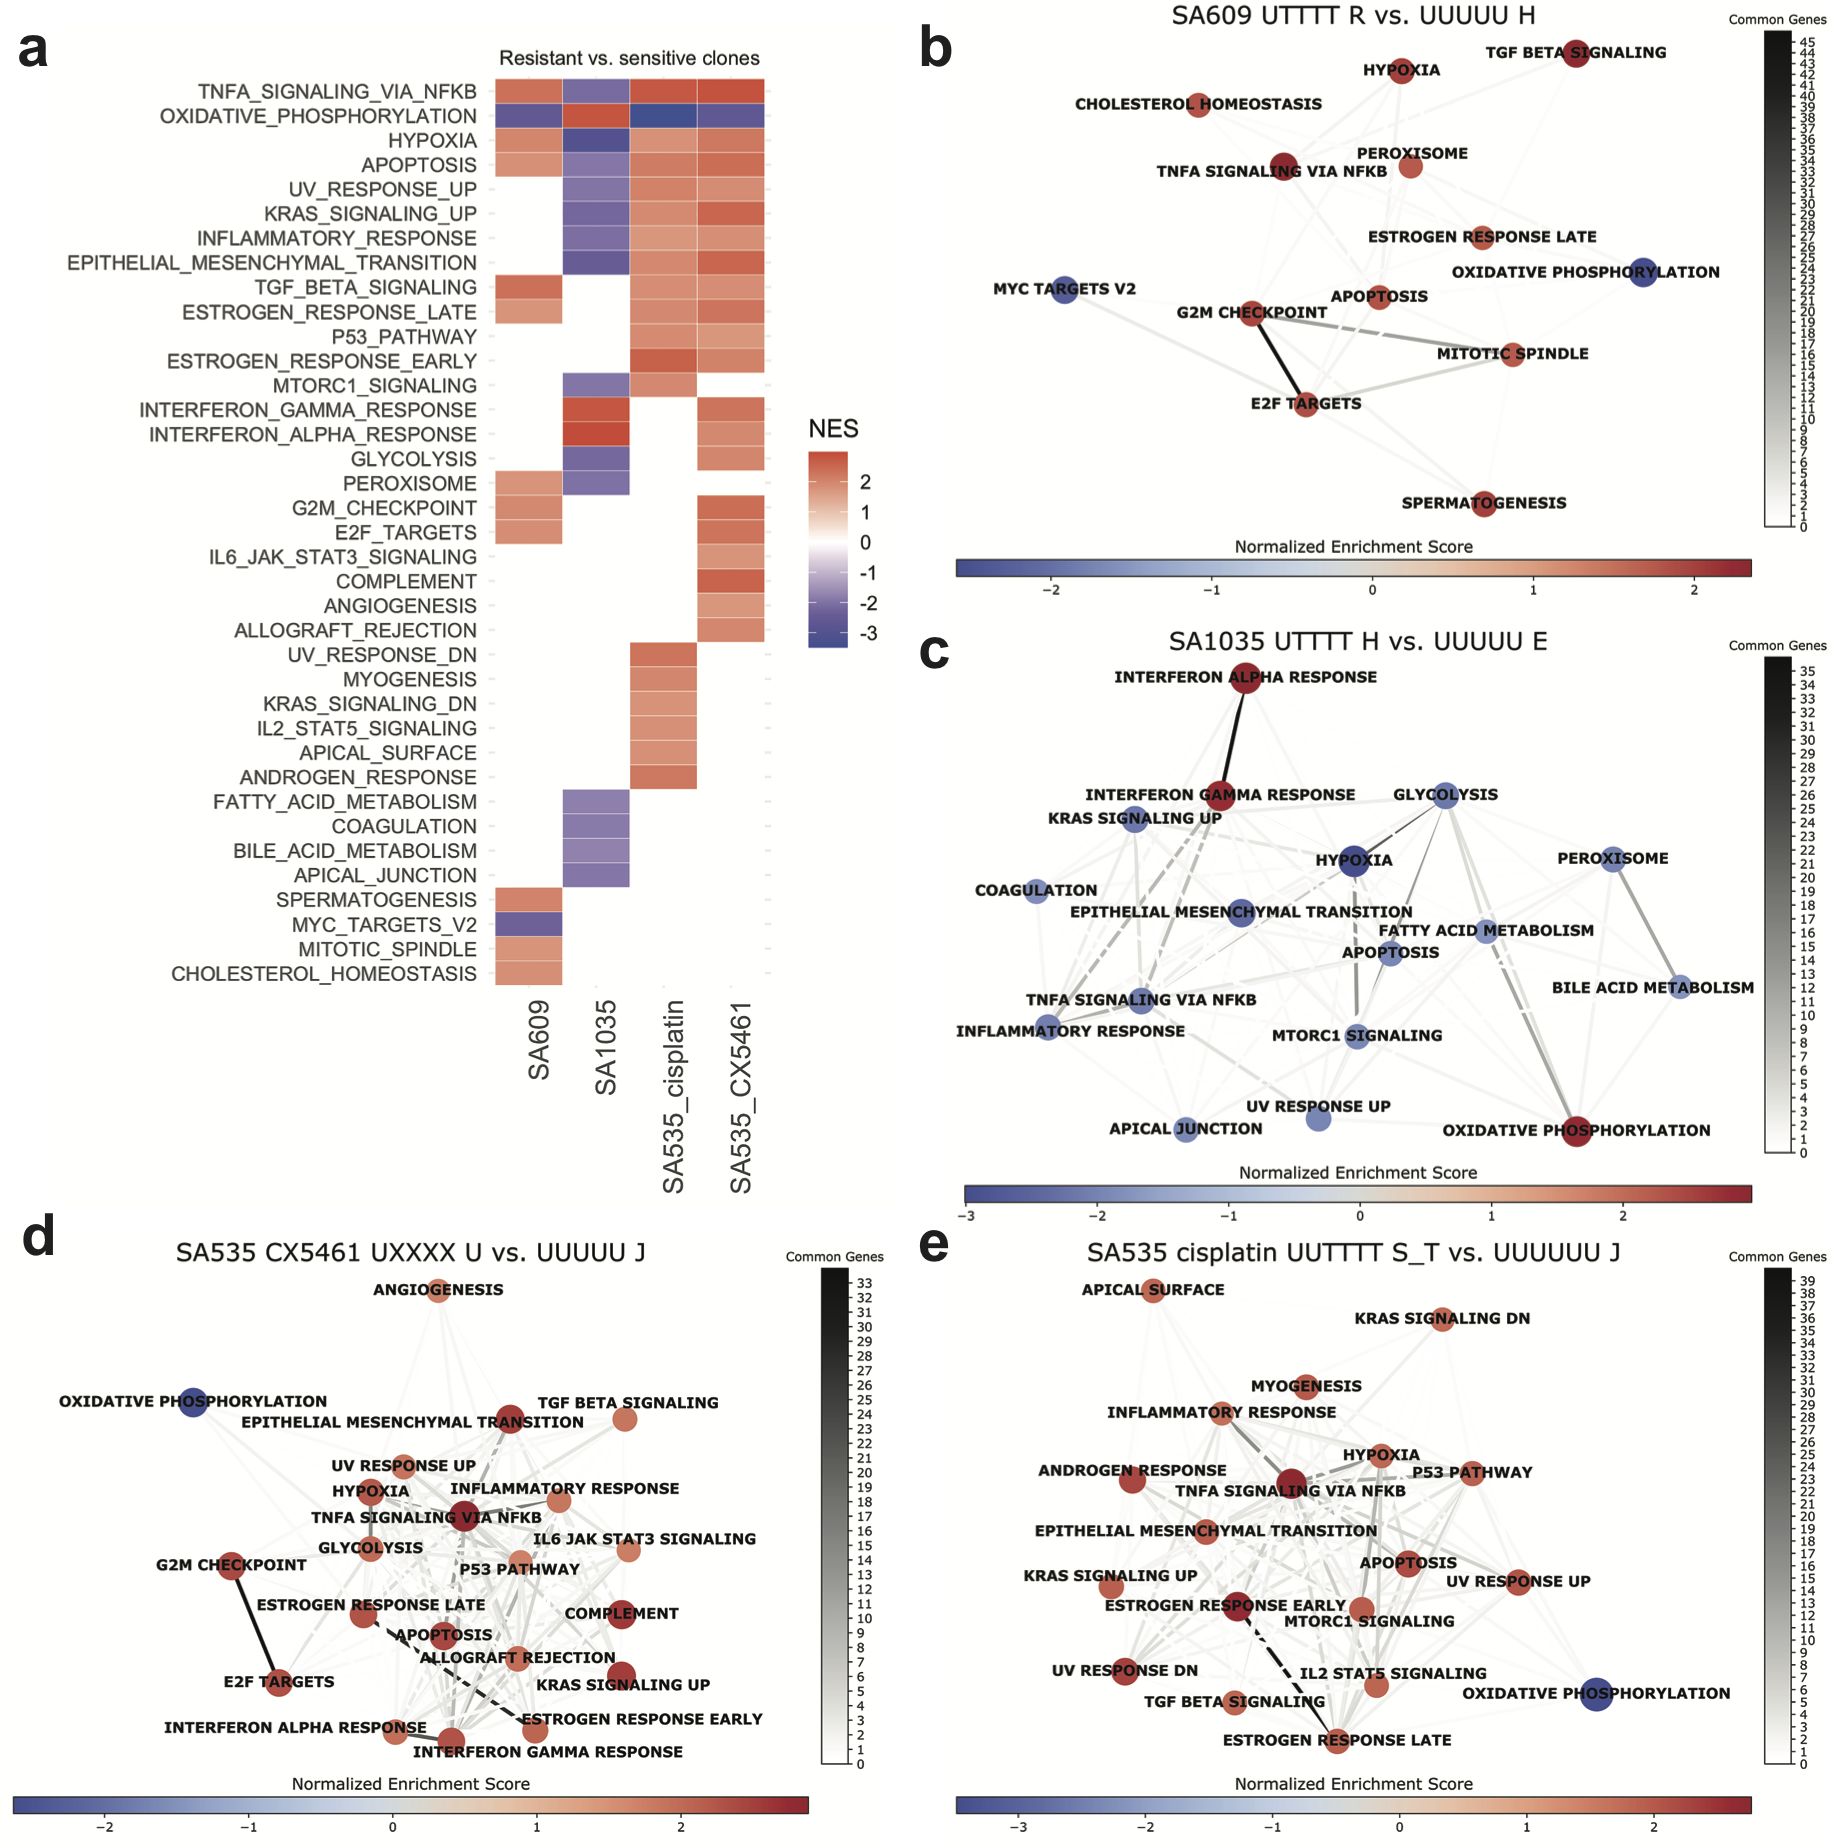
\includegraphics[width=\textwidth]{Figures/chap5/pathwaysnetwork.png}
\caption[Gene pathway enrichment analysis of PDX timeseries]
	{\small
	\textbf{Gene pathway enrichment analysis of PDX timeseries.}
	 	\textbf{(a)} Vertical axis on the left enlists the pathways involved from a ranked gene set enrichment analysis (GSEA) \cite{shi2007gene}. Horizontal axis denotes the IDs of TNBC PDX. Colour intensity identifies normalized enrichment score (NES) obtained by using all the differentially expressed genes at time points X7 for TNBC-SA609, X8 for TNBC-SA1035, X9 for TNBC-SA535-cisplatin and X8 for TNBC-SA535-CX-5461 at p-value $\leq 0.001$. The hallmark gene set collection from MSigDB \cite{liberzon2015molecular} was used. Significantly enriched pathways (p-value $<$ 0.05) were retained.   \textbf{(b-e)} Networks showing the relationship between the enriched pathways in \textbf{a}. The grey to black lines indicate the number of genes shared between pathways. \textbf{(b)} TNBC-SA609. \textbf{(c)} TNBC-SA1035.  \textbf{(d)} TNBC-SA535-CX-5461. \textbf{(e)} TNBC-SA535-cisplatin.
	}
	\label{fig:pathwaysnetwork}
\end{figure}

%------------------------------------------------------------------



\subsection{Integrated transcriptome and pathway analyses revealed potential genes and key activated pathways in breast cancer}
%Next, we performed gene set enrichment analysis (GSEA) to search for sets of genes that are significantly over-represented in a given list of genes, compared to a background set of genes and their respective pathways and network connections. 
%First, We generated a heatmap of pathway evolution from one treated time point to another in all timeseries TNBC PDX \textbf{\autoref{fig:pathwaysevolution}}. Most of the listed pathways were enriched at the later timepoints, where tumors started developing chemoresistance. 

\subsubsection{Profiling of signaling pathways reveals a distinct demarcation between SA1035 and rest of 3 TNBC PDX}
To assess the common pathways and their network connections, 
we profiled pathway enrichment scores between the resistant and sensitive clones of all TNBC PDX at the late time points:  X7 for TNBC-SA609, X8 for TNBC-SA1035, X9 for TNBC-SA535-cisplatin and X8 for TNBC-SA535-CX-5461 (\textbf{\autoref{fig:pathwaysnetwork}}). 
Pathway specific differentially expressed genes were included in network enrichment analysis and the nodes were coloured by the normalized enrichment score (NES). Interestingly, TNBC-SA1035 PDX demonstrated only three upregulated pathways in resistant versus sensitive clone, including \textbf{Oxidative phosphorylation (OXPHOS)}, \textbf{Interferon alpha response} \cite{provance2019deciphering} and \textbf{Interferon gamma response} \cite{mojic2018dark} (\textbf{\autoref{fig:pathwaysnetwork} a}, second column). \textbf{\ac{OXPHOS}} is known to be upregulated in cisplatin related drug resistance mechanism \cite{lee2017myc}. The latter two pathways are not well studied in relation to tumor progression or drug resistance but there is some speculative research related to these interferons and cancer related immune mechanisms. In contrast to other TNBC PDX, TNBC-SA1035 resistant clone also evinced downregulated pathways of \textbf{Hypoxia}, \textbf{TNFA signaling via NF-$\kappa$B}, \textbf{\ac{EMT}}, \textbf{MTORC1 signaling}, \textbf{KRAS signaling} and \textbf{Apoptosis} ({\textbf{\autoref{fig:pathwaysnetwork} c}}). The genes involved in these pathways are shown in \textbf{\autoref{fig:genenetworkanalysis} b}.

In addition to TNBC-SA1035, only TNBC-SA535 timeseries that was treated with CX-5461 showed interferons pathways upregulation. However, the rest of 3 TNBC PDX, TNBC-SA609, TNBC-SA535-cisplatin treated and TNBC-SA535-CX-5461 treated, showed commonly upregulated certain pathways, including, \textbf{TNFA signaling via NF-$\kappa$B} \cite{lagunas2008nuclear,ito2015down, ryan2019targeting}, \textbf{Hypoxia} \cite{lee2012hypoxia, mcevoy2015identifying, deben2018hypoxia,li2019erk}, \textbf{Apoptosis} \cite{panaretakis2012cisplatin}, \textbf{TGF Beta signaling} \cite{zhang2019tgfbeta1} and \textbf{Estrogen response} \cite{zhu2018er}. \textbf{E2F targets} \cite{zheng2020upregulation} and \textbf{G2M checkpoint} \cite{visconti2016cell} were common between TNBC-SA609 and TNBC-SA535-CX-5461 treated (\textbf{\autoref{fig:pathwaysnetwork} a}, first, third and fourth columns). 



\begin{figure}
\centering
  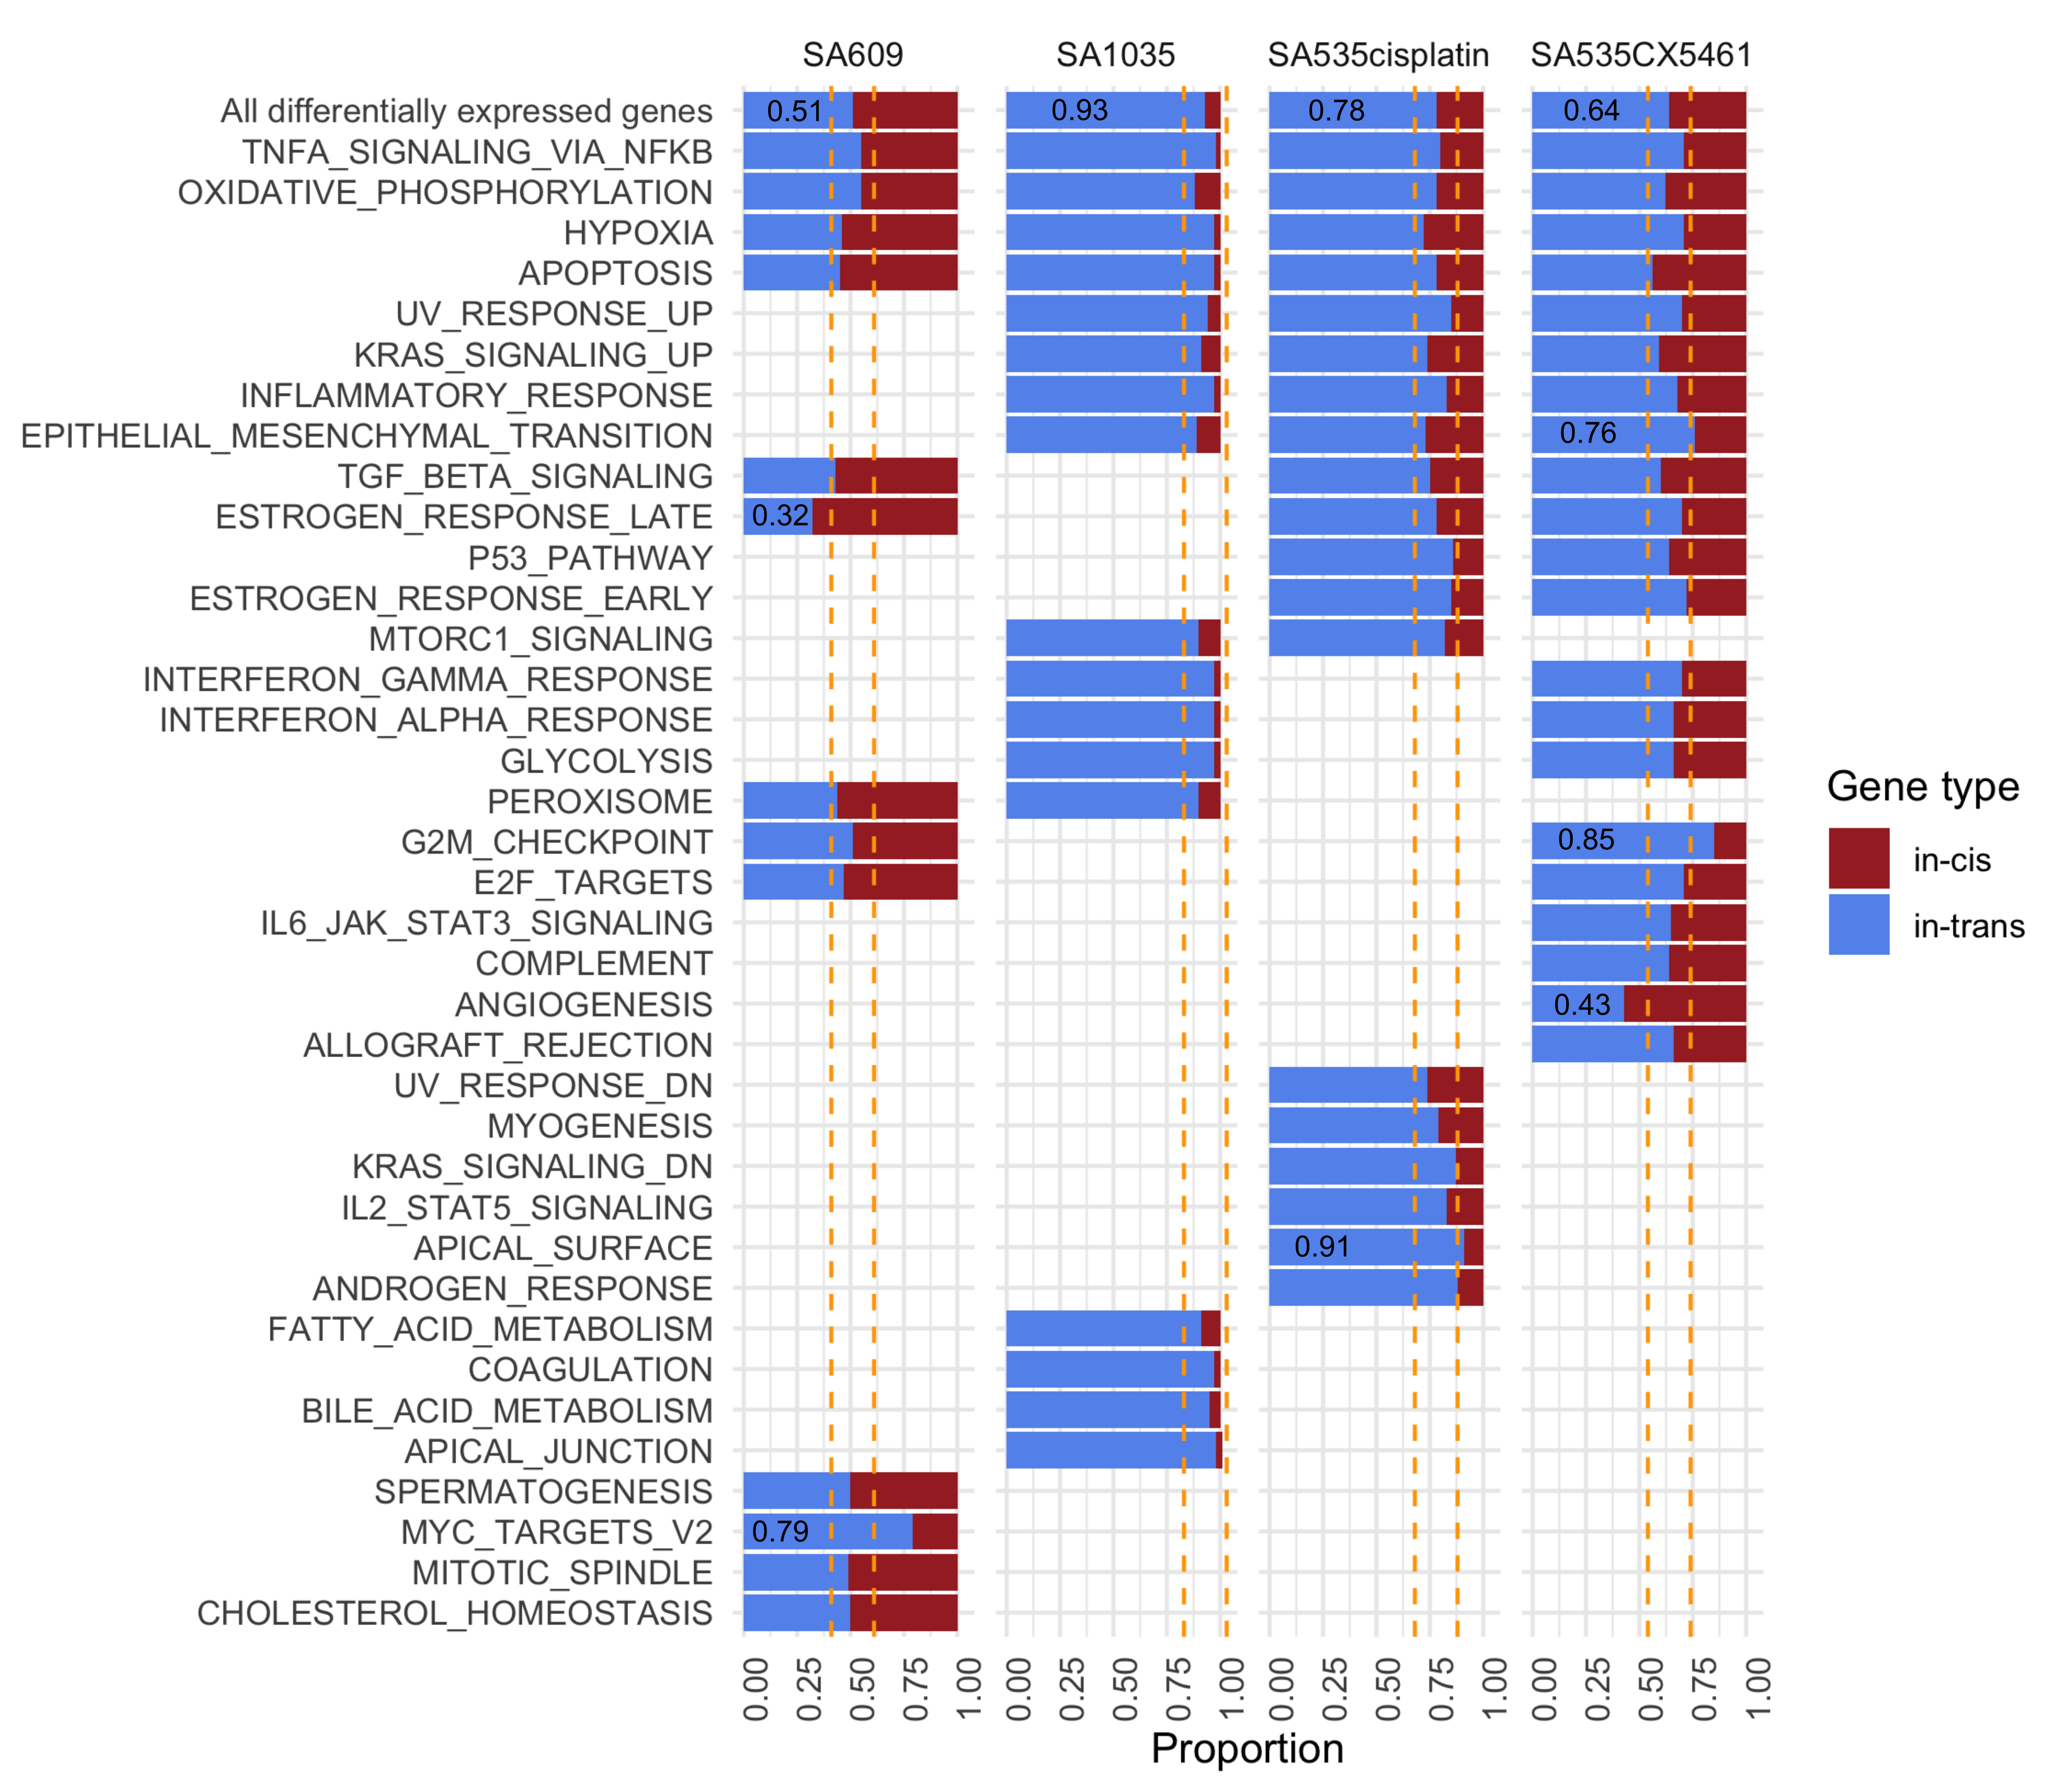
\includegraphics[width=\textwidth]{Figures/chap5/cistransproportionsinpathways.png}
\caption[Proportions of \textit{in cis} and \textit{in trans} regulated genes in pathways]
	{\small
	\textbf{Proportions of \textit{in cis} and \textit{in trans} regulated genes in pathways.}
	 	Vertical axis on the left enlists the gene set enrichment analysis (GSEA) pathways in the same order as in \textbf{\autoref{fig:pathwaysnetwork}}, with the addition of a new row on top for all the differentially expressed genes. For each set of genes and each series, the proportion of \textit{in cis} (red) and \textit{in trans} (blue) genes was calculated. The \textit{in trans} proportions for all genes (top row) are given. Vertical dashed lines show the expected proportions, defined as the proportions in all genes (top row), plus or minus 10\%. The observed proportions outside of this range are identified. 
	}
	\label{fig:cistransproportionsinpathways}
\end{figure}


%---------------------------------------------------------------------

% text about the in-cis in-trans proportions figure 
The proportions of \textit{in cis} and \textit{in trans} genes in the gene set enrichment pathways are within 10\% of the proportion in the entire population of genes for most pathways, with only a few exceptions (\textbf{\autoref{fig:cistransproportionsinpathways}}). In TNBC-SA609 (expected \textit{in trans} proportion 0.51), \textbf{Estrogen response late} pathway has a lower percentage of \textit{in trans} genes (0.32), while \textbf{MYC targets V2} has a higher percentage of \textit{in trans} genes (0.79). In TNBC-SA1035 all pathway proportions are within the expected range (0.93 \textit{in trans} proportion). In TNBC-SA535-cisplatin (expected \textit{in trans} proportion 0.78), only \textbf{Apical surface} pathway has a higher \textit{in trans} proportion of 0.91. Finally, in TNBC-SA535-CX-5461 (expected \textit{in trans} proportion 0.78), \textbf{EMT} and \textbf{G2M checkpoint} pathways have a higher \textit{in trans} proportion (0.76 and 0.85, respectively), and \textbf{Angiogenesis} has a lower \textbf{in trans} proportion of 0.43.

To portray pathway specificity in resistant versus sensitive clones, we explored \textbf{SA609 TNBC PDX}, which was  comprised of \textbf{TGF Beta signaling, Hypoxia, TNFA signaling via NF-$\kappa$B, Cholesterol homeostasis, Peroxisome} and \textbf{Apoptosis} (\textbf{\autoref{fig:pathwaysnetwork} b}). In addition to these, \textbf{G2M checkpoint} and \textbf{E2F targets} were found to be upregulated with $>$40 common genes between these two pathways. \textbf{Mitotic spindle} pathway upregulation was also associated with sharing of $>$10 genes with \textbf{E2F} and \textbf{G2M check point} pathways \textbf{\autoref{fig:genenetworkanalysis} a}.

%--------------------------------------------------------------------

\subsubsection{TNBC-SA535 PDX reveals specificity of drugs in pathway network inference} 
As \textbf{TNBC-SA535 PDX} was treated with two different drugs, cisplatin and CX-5461 in parallel (\textbf{\autoref{fig:SA535CX5461} a}), we explored how many pathways are comparable in these two series and which ones are distinct or unique to each specific drug. 
We found that \textbf{11 pathways} were upregulated and only one, which was \textbf{\ac{OXPHOS}}, was down regulated in both series, suggesting their specificity to the tumor itself. The list of these pathways encompass \textbf{TNFA signaling via NF-$\kappa$B, Hypoxia, Apoptosis, UV response up, KRAS signaling up, Inflammatory response, Epithelial mesenchymal transition, TGF Beta signaling, Estrogen response} and \textbf{p53} pathways ({\textbf{\autoref{fig:pathwaysnetwork} a} third \& fourth column upper half and \textbf{\autoref{fig:pathwaysnetwork} d, e}). However, there were certain pathways that were definitive to one of the two drugs. The cisplatin treated resistant clone was found to have exclusively upregulated pathways including \textbf{MTORC1 signaling \cite{peng2010role}, KRAS signaling down} \cite{tao2014oncogenic}, \textbf{IL-2\_STAT5 signaling \cite{wu2020activation, gutierrez2020role}, Apical surface} (genes encoding proteins over-represented on the apical surface of epithelial cells, e.g., apical area important for cell polarity) \cite{halaoui2015rewiring, wodarz2007cell}, \textbf{UV response down} (including \textbf{UV\_response\_Via\_ERCC3\_TTD\_DN}
and \textbf{UV\_response\_Via\_ERCC3\_XPCS\_DN}) and \textbf{Androgen response} pathways \cite{rampurwala2016role, michmerhuizen2020we}.}

Within cisplatin treated activated pathways, \textbf{Hypoxia, TNFA signaling via NF-$\kappa$B, MTORC1, Estrogen response} and \textbf{Inflammatory response} related pathways share the most common genes among their network (\textbf{\autoref{fig:pathwaysnetwork} e}). The genes that are expressed are shown in  \textbf{\autoref{fig:genenetworkanalysis} c}. However, CX-5461 treated resistant clone came up particularly with \textbf{G2M checkpoint, E2F targets, IL-6\_JAK\_STAT3 signaling, Angiogenesis, Complement system} (genes encoding components of the complement system, which is part of the innate immune system), \textbf{Interferon alpha response, Interferon gamma response} and \textbf{Glycolysis} (\textbf{\autoref{fig:pathwaysnetwork} d}). Among these pathways, \textbf{G2M checkpoint} and \textbf{E2F targets} pathways share $>$30 genes, whereas, \textbf{\ac{EMT}, TNFA signaling via NF-$\kappa$B, Hypoxia} and \textbf{Glycolysis} share $>$ 15 genes. The gene network with related pathways are shown in  \textbf{\autoref{fig:genenetworkanalysis} d}. 

%-------------------------------------------------------------------
\begin{figure}
\centering
 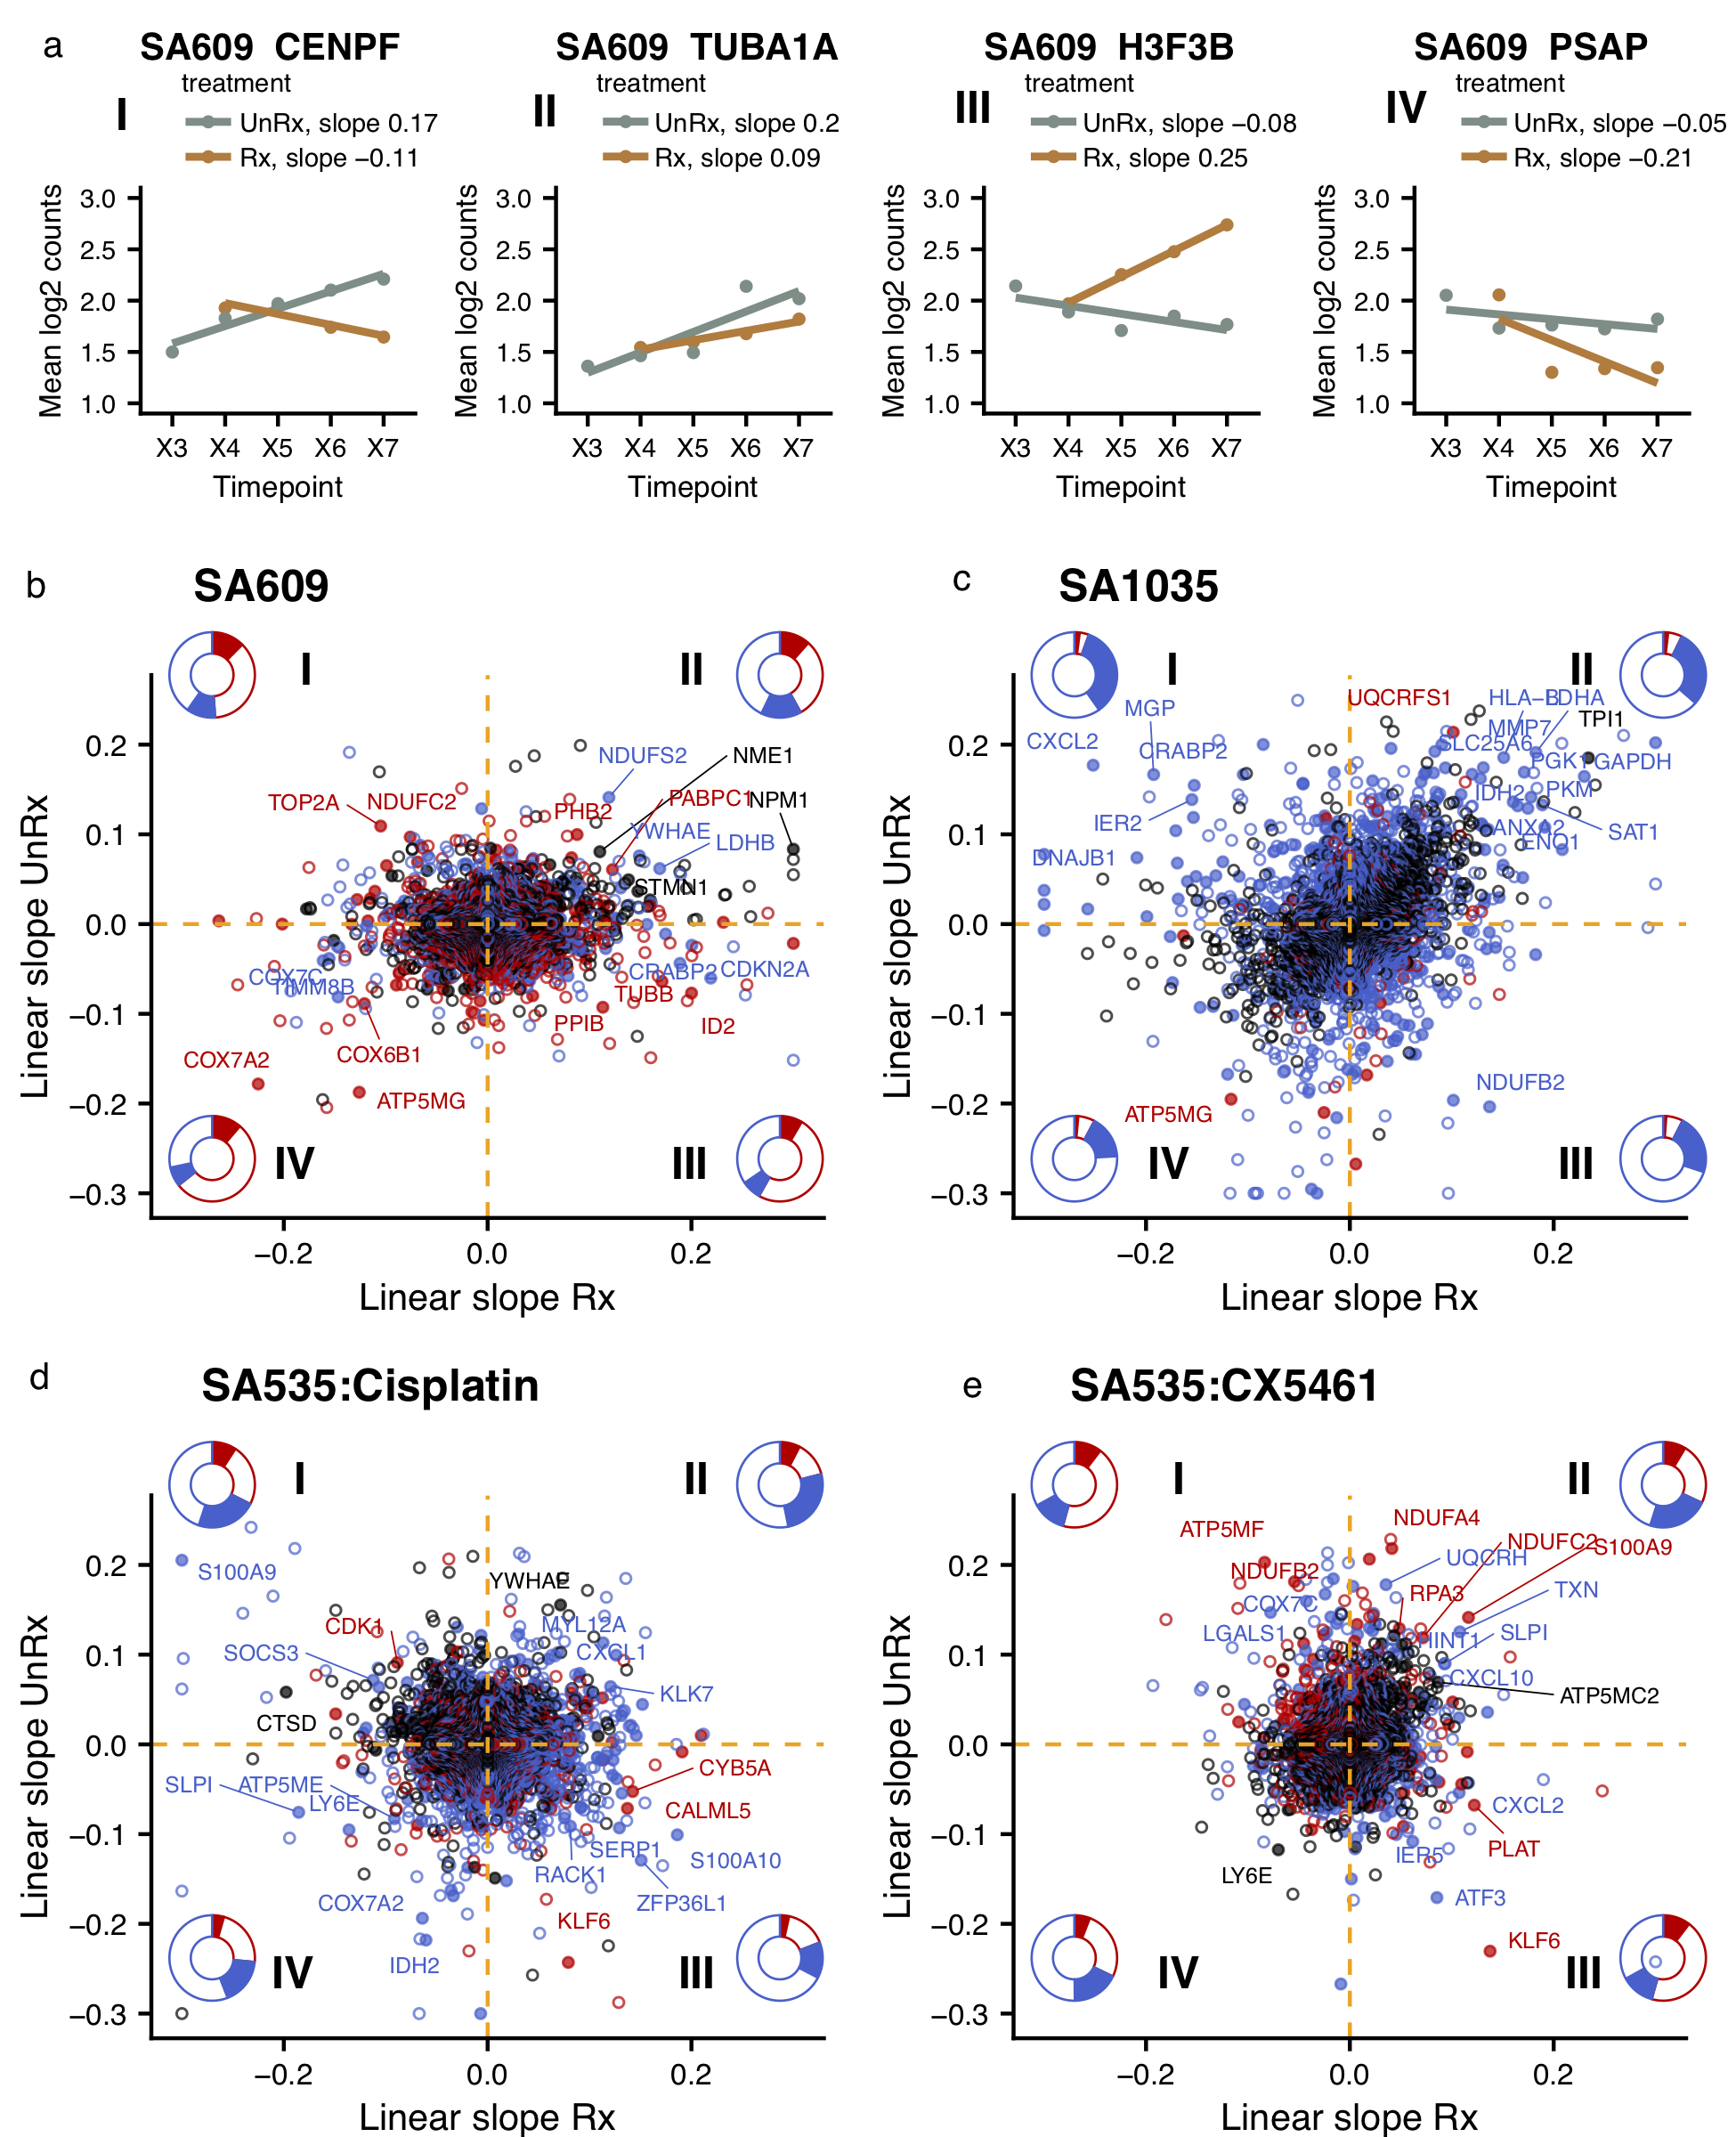
\includegraphics[width=\textwidth]{Figures/chap5/GeneschanginginRxclouds.png}
\caption[Gene expression changes over time with or without treatment in all 4 TNBC PDX timseries]
	{\small
	 \textbf{Gene expression changes over time with or without treatment in all 4 TNBC PDX timseries}.
Density plots of linear slopes showing the gene expression change across treatment cycles (x-axis) versus linear slopes showing gene expression change across untreated time points (y-axis). Unless otherwise noted, the slopes were calculated by fitting a linear model to mean SCTransform log2 normalized gene expression levels at time points UT, UTT, UTTT and UTTTT for treated, and at time points U, UU, UUU, UUUU and UUUUU for untreated. Each of the four quadrants are numbered as I (includes genes increasing in untreated passaging and decreasing with treatment), II (increasing both in untreated as well as with treatment), III (increasing expression only with treatment and decreasing without drug) and  IV (decreasing with passaging over time in both untreated and treated tumors).  \textbf{(a)} TNBC-SA609 . \textbf{(b)} TNBC-SA1035, UT and UU were eliminated from the slope calculation due to lower data quality. \textbf{(c)} TNBC-SA535-cisplatin. \textbf{(d)} TNBC-SA535-CX-5461, slopes were calculated at time points UX, UXX and UXXXX, the available data for this series.}

	\label{fig:GeneschanginginRxclouds}
\end{figure}

%-------------------------------------------------------------------

\subsubsection{Gene specific expression trajectories exemplified systematic response to sustained treatment}
%To understand the stability of gene expression throughout the treatment, we performed gene regression analysis on the top 500 resistant clone related genes and plotted their trend along various timepoints. All four treated PDX series manifested 2-3 distinct clusters with monotonically increasing, monotonically decreasing, remaining constant or irregular patterns \textbf{\autoref{fig:GeneschanginginRxclouds}}. Some of the gene clusters were found to be increasing or decreasing along the time series of the PDX models and require detailed investigation at individual gene level to get enough evidence.

To understand the gene expression dynamics over several treatment cycles in comparison with gene expression in consecutive untreated time points, we performed linear model fitting over the mean SCTransform log2 normalized gene expression levels at 3-5 time points (\textbf{\autoref{fig:GeneschanginginRxclouds}}). The slope of the linear fitting signifies the overall magnitude of change from one time point to the next. Since the y axis is on a log2 scale, a slope of 1 means that, on average over time, the expression level doubles with every time point. Similarly, slopes 0.1 and 0.2 mean that, on average, the expression level increases by 7\% and 15\%, respectively, at every time point.

\textbf{\autoref{fig:GeneschanginginRxclouds}} shows the untreated slope (y axis) versus the treated slope (x axis) for each gene in our four series, with the \textit{in cis} and \textit{in trans} genes shown in red and blue colours, respectively. The genes in quadrants II and IV changed in the same direction in both treated and untreated (up in II and down in IV), suggesting dynamics due to passage, and not due to treatment status. Conversely, the genes in quadrants I and III changed in the opposite direction in the treated samples versus the untreated samples, suggesting dynamics due to treatment status. While the vast majority of genes form a "cloud" around the origin, a number of genes display significant changes.

 
To evaluate the spectrum of single gene expression at each time point, we designated at least 4 genes from each of the 4 TNBC PDX from the linear model analysis (\textbf{\autoref{fig:GeneschanginginRxclouds},\autoref{tab:selected4genestable}}). Summary of top 20 significantly upregulated and downregulated genes of all cisplatin treated PDX timeseries are enlisted in \textbf{\autoref{tab:SA609upregulatedgenesinclusters}, \autoref{tab:SA609downrregulatedgenesinclusters}, \autoref{tab:SA1035upregulatedgenesinclusters}, \autoref{tab:SA1035downregulatedgenesinclusters}, \autoref{tab:SA535upregulatedgenesinclusters}, \autoref{tab:SA535downregulatedgenesinclusters}}.

%-------------------------------------------------------------

 % Table generated by Excel2LaTeX from sheet 'Sheet1'
 \begin{table}[htbp]
   \centering
   \caption{Upregulated 4 cancer related significant genes selected from cloud plots in each of 4 PDX timeseries}
     \begin{tabular}{|r|l|l|}
     \hline
     \multicolumn{1}{|l|}{TNBC PDX ID} & Selected gene ID & Gene\_Regulation \\
     \hline
     \multicolumn{1}{|l|}{TNBC-SA609} & ID2 & in trans-upregulated \\
       & FIS1  & in cis-upregulated \\
       & CRABP1  & in trans-upregulated \\
       & MYC  & in trans-upregulated \\
     \multicolumn{1}{|l|}{TNBC-SA1035} & MDK & in trans-upregulated \\
       & NDUFB4  & in cis-upregulated \\
       & COX6C  & in cis-upregulated \\
       & UQCRB  & in cis-upregulated \\
     \multicolumn{1}{|l|}{TNBC-535-cisplatin} & BCAP31 & in cis-upregulated \\
       & RHOB  & in cis-decrease-upregulated \\
       & OLA1  & in cis-upregulated \\
       & METTL5  & in cis-upregulated \\
     \multicolumn{1}{|l|}{TNBC-535-CX-5461} & ID2  & in cis-decrease-upregulated \\
       & TOP2A  & in trans-upregulated \\
       & MARCKS  & in trans-upregulated \\
       & BUB1  & in trans-upregulated \\
       \hline
     \end{tabular}%
   \label{tab:selected4genestable}%
 \end{table}%
%-------------------------------------------------------------
\begin{figure}
\centering
 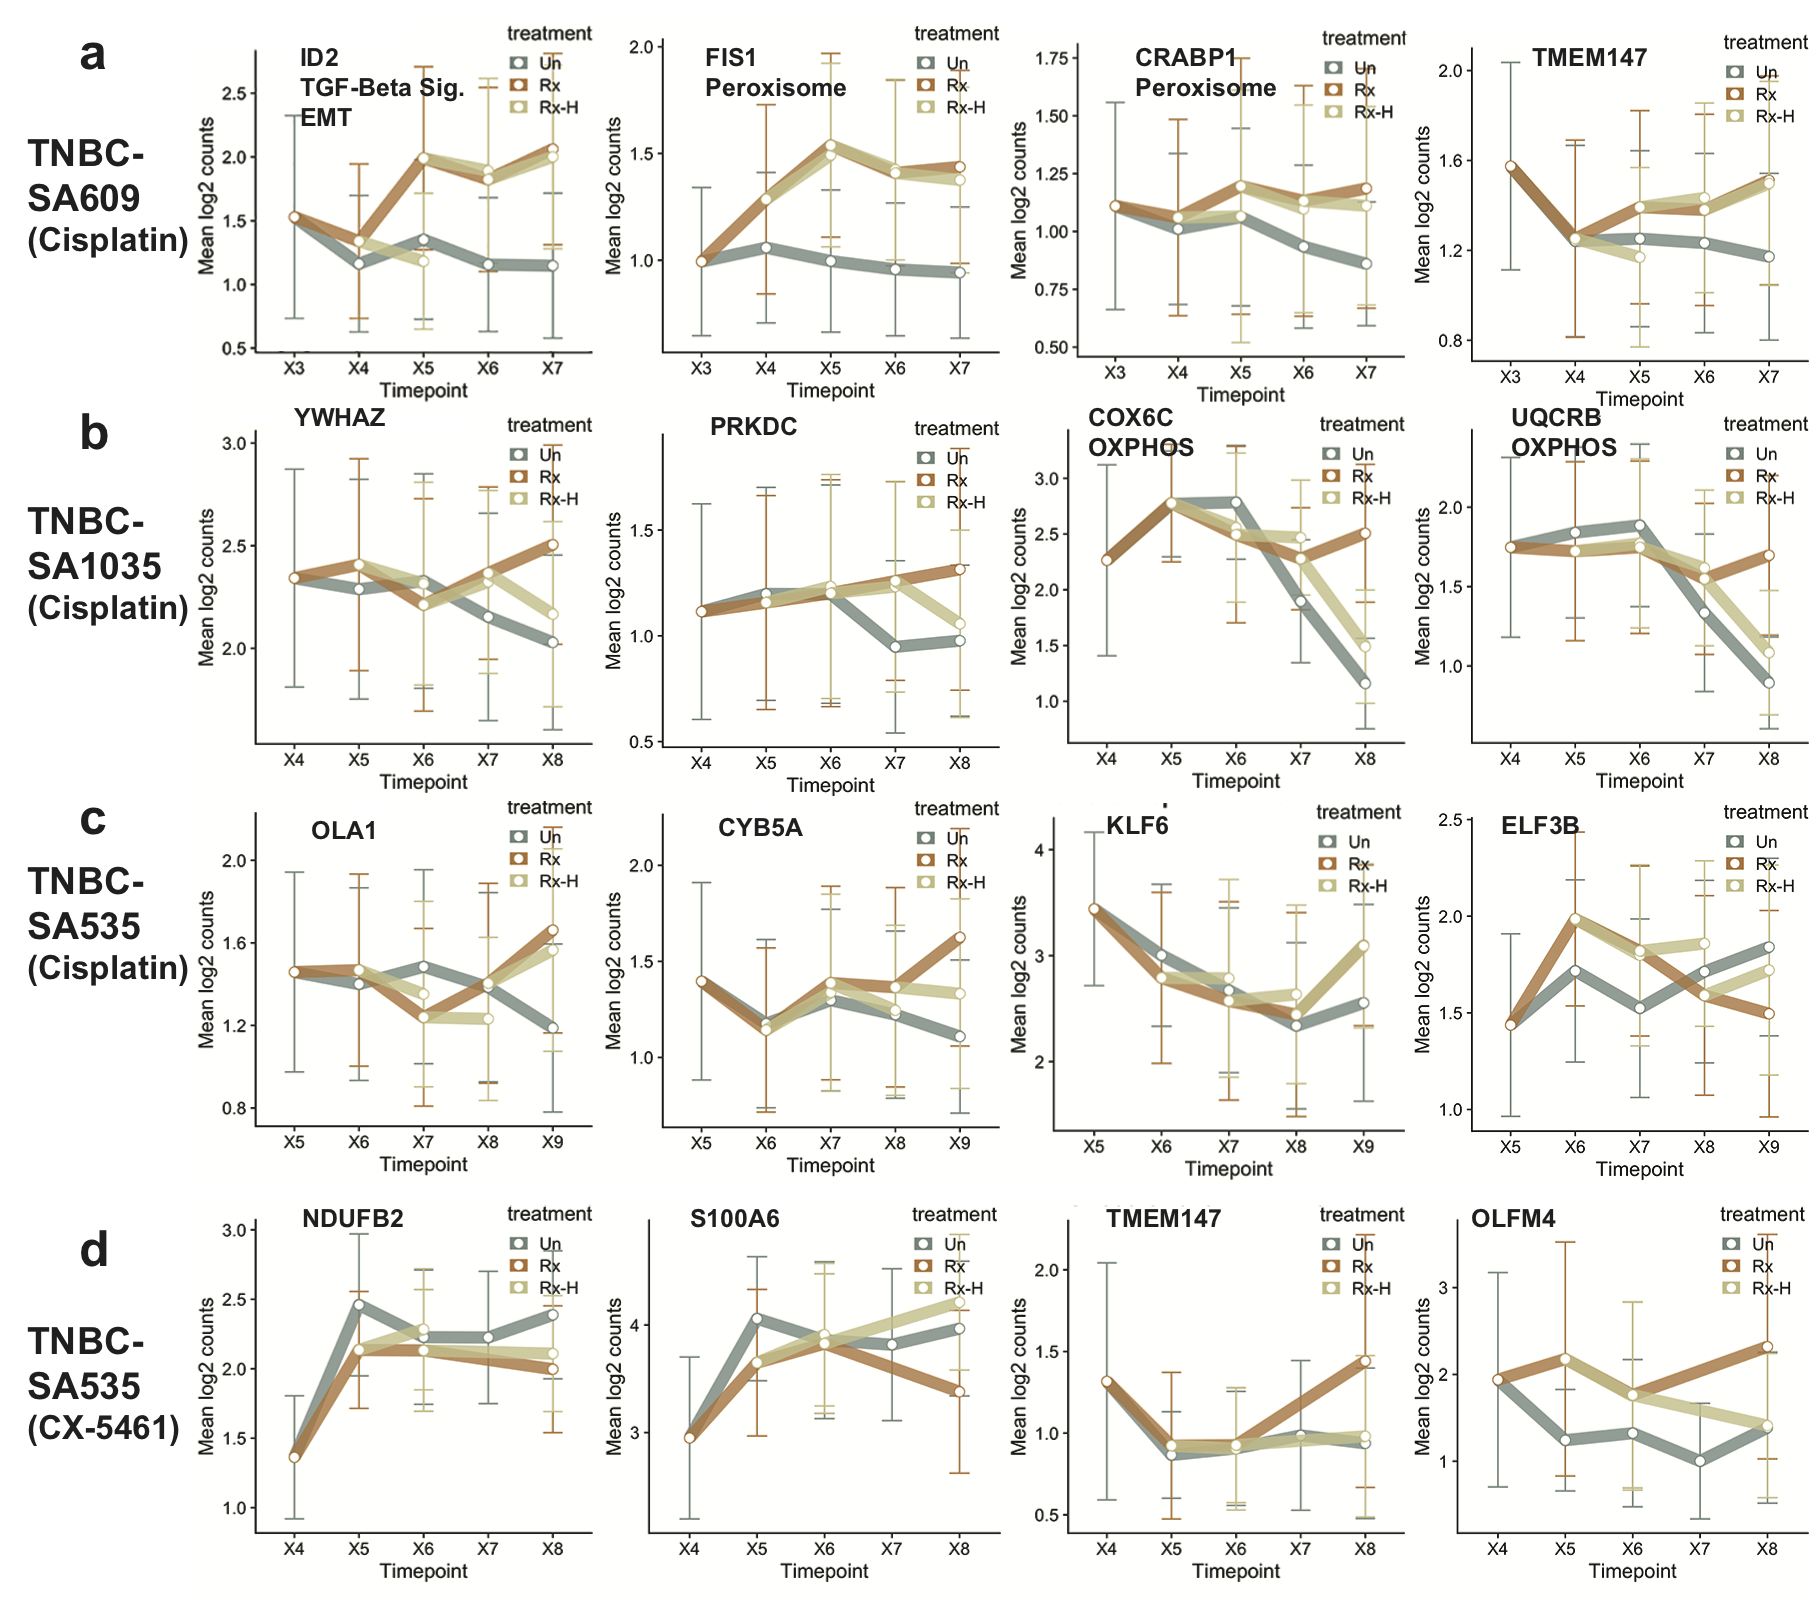
\includegraphics[width=\textwidth]{Figures/chap5/incisgenelinetrajectories.png}
	
\caption[Four \textit{in cis} gene expression changed over time]
	{\small
	 \textbf{Selected four \textit{in cis} regulated gene expression changes over time in all timeseries PDX}.
	Horizontal axis represents time point passages while vertical axis denotes SCTransform normalized mean log2 count of single cell expression level. Three line trajectories indicates treated, un-treated and drug-holiday samples. }

	\label{fig:incisgenelinetrajectories}
\end{figure}
%----------------------------------------------------------------

\begin{figure}
\centering
 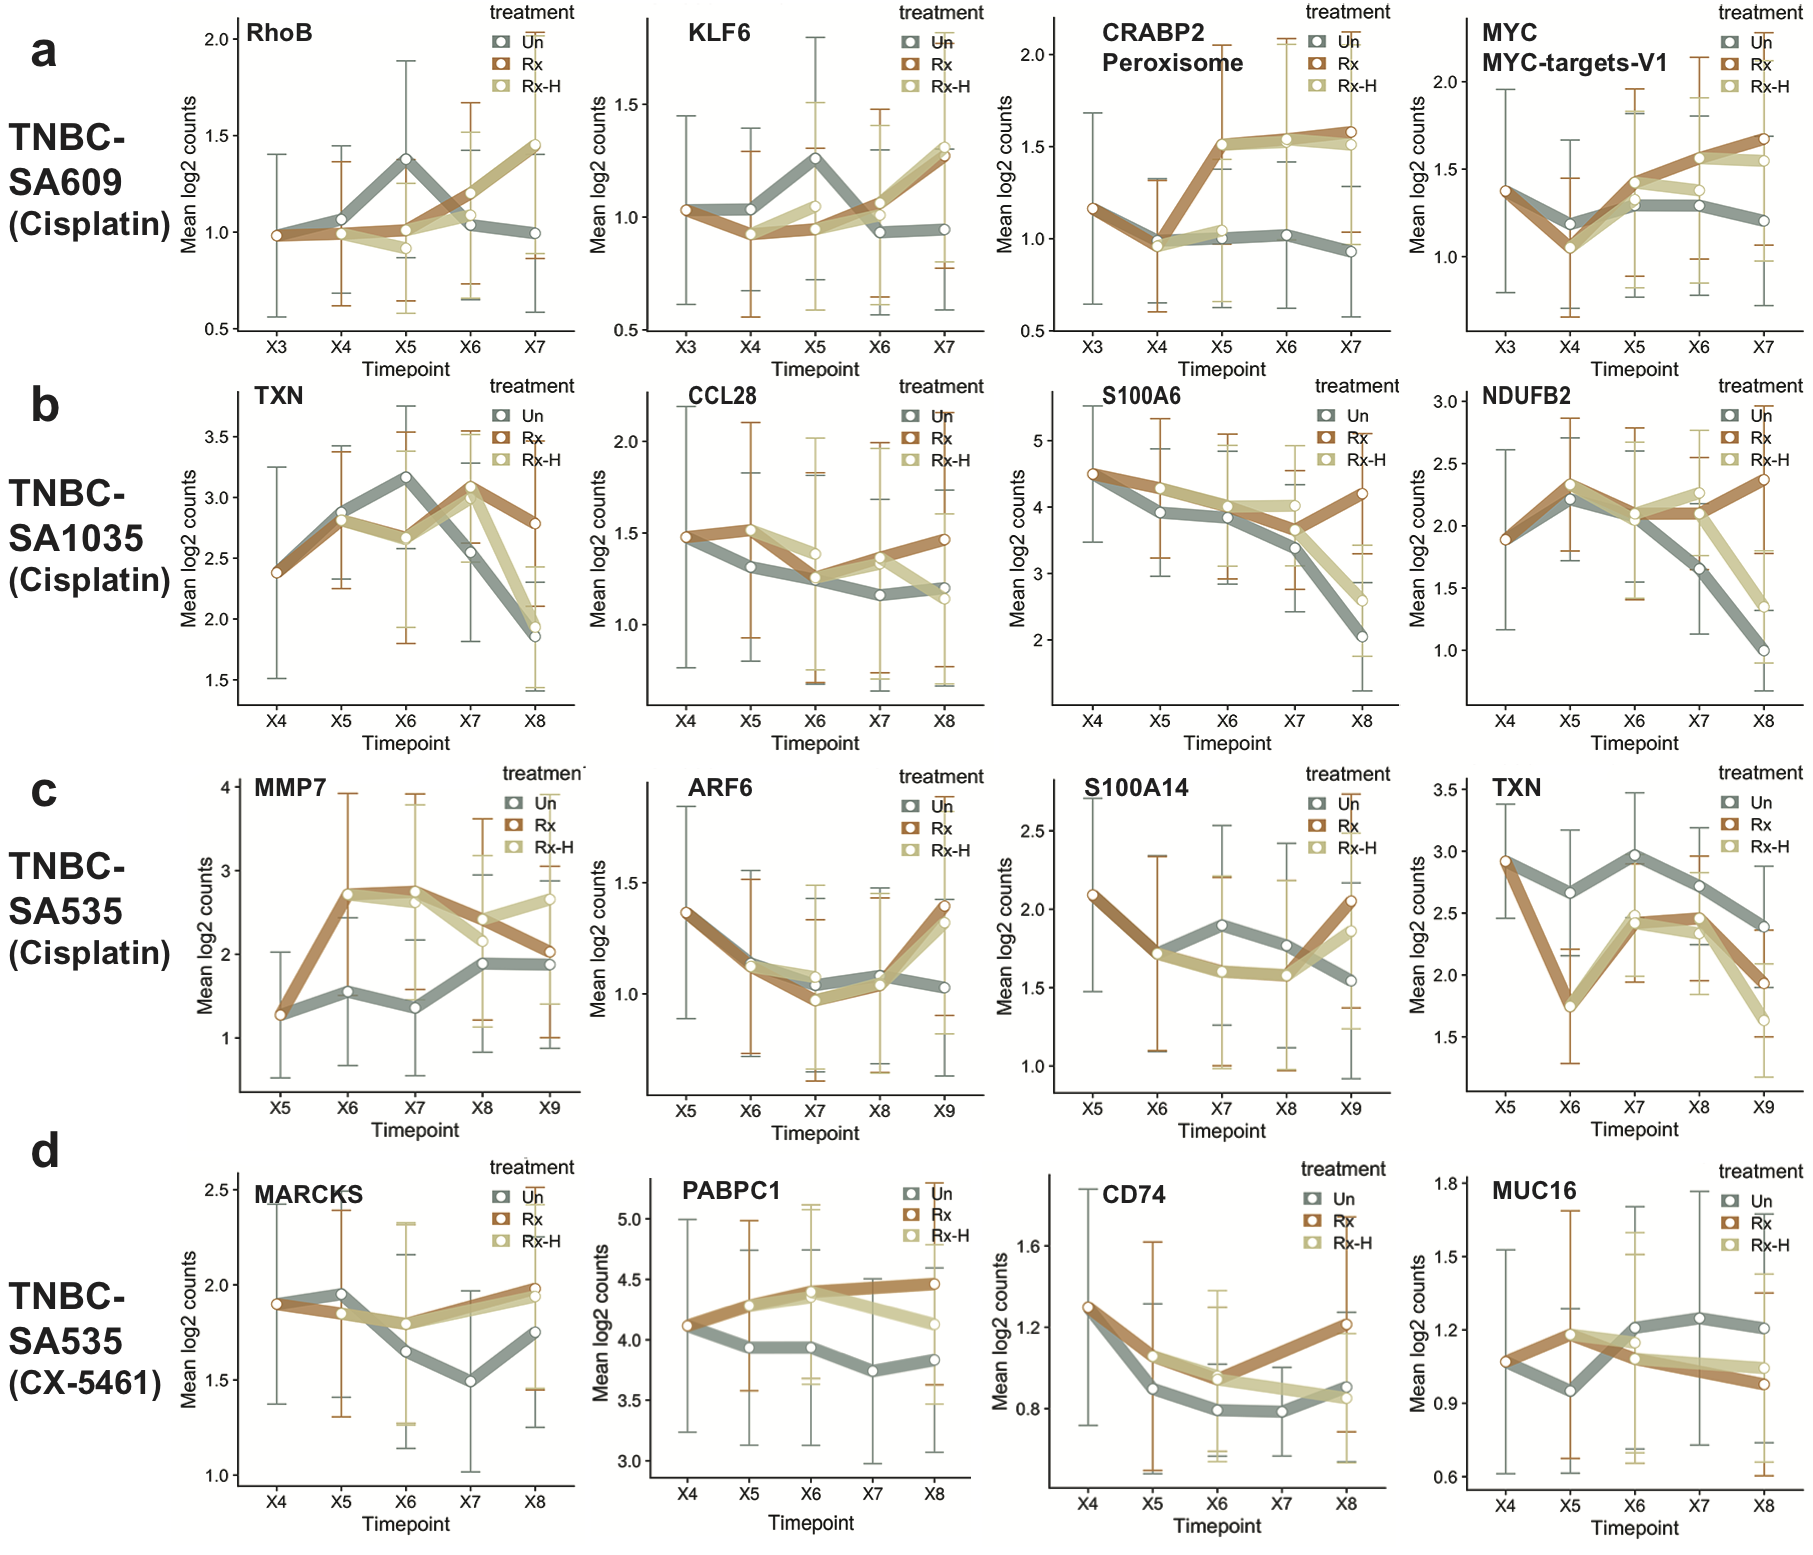
\includegraphics[width=\textwidth]{Figures/chap5/Intransgenelinetrajectories.png}
	
\caption[Four \textit{in trans} gene expression changed over time]
	{\small
	 \textbf{Selected four \textit{in trans} regulated gene expression changes over time in all timeseries PDX}.
	Horizontal axis represents time point passages while vertical axis denotes SCTransform normalized mean log2 count of single cell expression level. Three line trajectories indicates treated, un-treated and drug-holiday samples. }

	\label{fig:Intransgenelinetrajectories}
\end{figure} 

 
 From TNBC-SA609, \textbf{DNA binding2 (ID2)} is shared between \textbf{TGF-Beta signaling and EMT} in our dataset. It is a key regulator of breast cancer metastasis to the brain. Overexpression of ID2 is known to increase proliferation, self-renewal, and expression of the putative stemness markers and inhibitors of DNA binding 2 represents a novel and promising therapeutic target for treating some of the cancers \cite{bae2017inhibitor, kijewska2019using}. This gene seems to be monotonically increasing from first cisplatin treatment cycle to the fourth. \textbf{Mitochondrial fission 1 (FIS1), peroxisome pathway}, is a mitochondrial dynamics-regulating gene, also found to be monotonically increasing with treatment cycle. Its overexpression prevents mitochondria elongation, which would otherwise lead to cell cycle delay or arrest \cite{fan2015mir, anderson2018dysregulation}. \textbf{CRABP1, peroxisome pathway} is an adverse prognostic factor and a potent inhibitor of retinoic acid (RA) action in breast cancer. It could serve as a biomarker to predict RA response \cite{liu2015crabp1}. \textbf{MYC} from \textbf{MYC targets V1}, another example of having monotonically increasing expression \textbf{\autoref{fig:generegressionanalysis} a-first panel}. It has been recently recognized that high MYC mRNA expression is more Clinically relevant than MYC DNA Amplification in triple-negative breast cancer \cite{chen2008myc, katsuta2020high}.

From TNBC-SA1035, we plotted timepoint trajectories of \textbf{MDK}, a growth factor, is recently reported as a key player in cancer progression and a promising therapeutic target \cite{filippou2020midkine}. It showed positive dynamics with continuous drug treatment. 
\textbf{NDUFB4, COX6C and UQCRB}, all from \ac{OXPHOS} pathway stayed very close to untreated expression levels in the initial few cycles but at the last time point, all of them diverges from untreated \textbf{\autoref{fig:generegressionanalysis} b.} Mitochondrial \textbf{UQCRB} is known as a molecular prognostic biomarker in colorectal cancer \cite{kim2017mitochondrial}.

From TNBC-SA535, we pulled out in total of 8 genes to demonstrate the change in expression in a time dependent manner. Cisplatin treated cycles includes, \textbf{BCAP31}, cancer/testis antigen-like protein, which drives TNBC development by modulating ligand-independent EGFR trafficking and spontaneous EGFR phosphorylation and it is known to act as a probe for non-small-cell lung cancer metastasis
\cite{fu2019bcap31, wang2020bcap31}. \textbf{TPT1} promotes tumorigenesis and metastasis in epithelial ovarian cancer \cite{wu2019lncrna}, seem to stay lower than the untreated but gradually kept on increasing till the last time point. \textbf{Obg-like ATPase 1 (OLA1)} overexpression predicts poor prognosis and promotes tumor progression by regulating P21/CDK2 in hepatocellular carcinoma \cite{huang2020obg}. Its expression was found to be increased in the last two cycles of cisplatin. \textbf{METTL5}, is known to promote translation initiation and breast cancer growth \cite{zeng2020roles}, also found to be increasing with increasing time points of treatment \textbf{\autoref{fig:generegressionanalysis} c.}

%----------------------------------------------------------------
\begin{figure}
\centering
  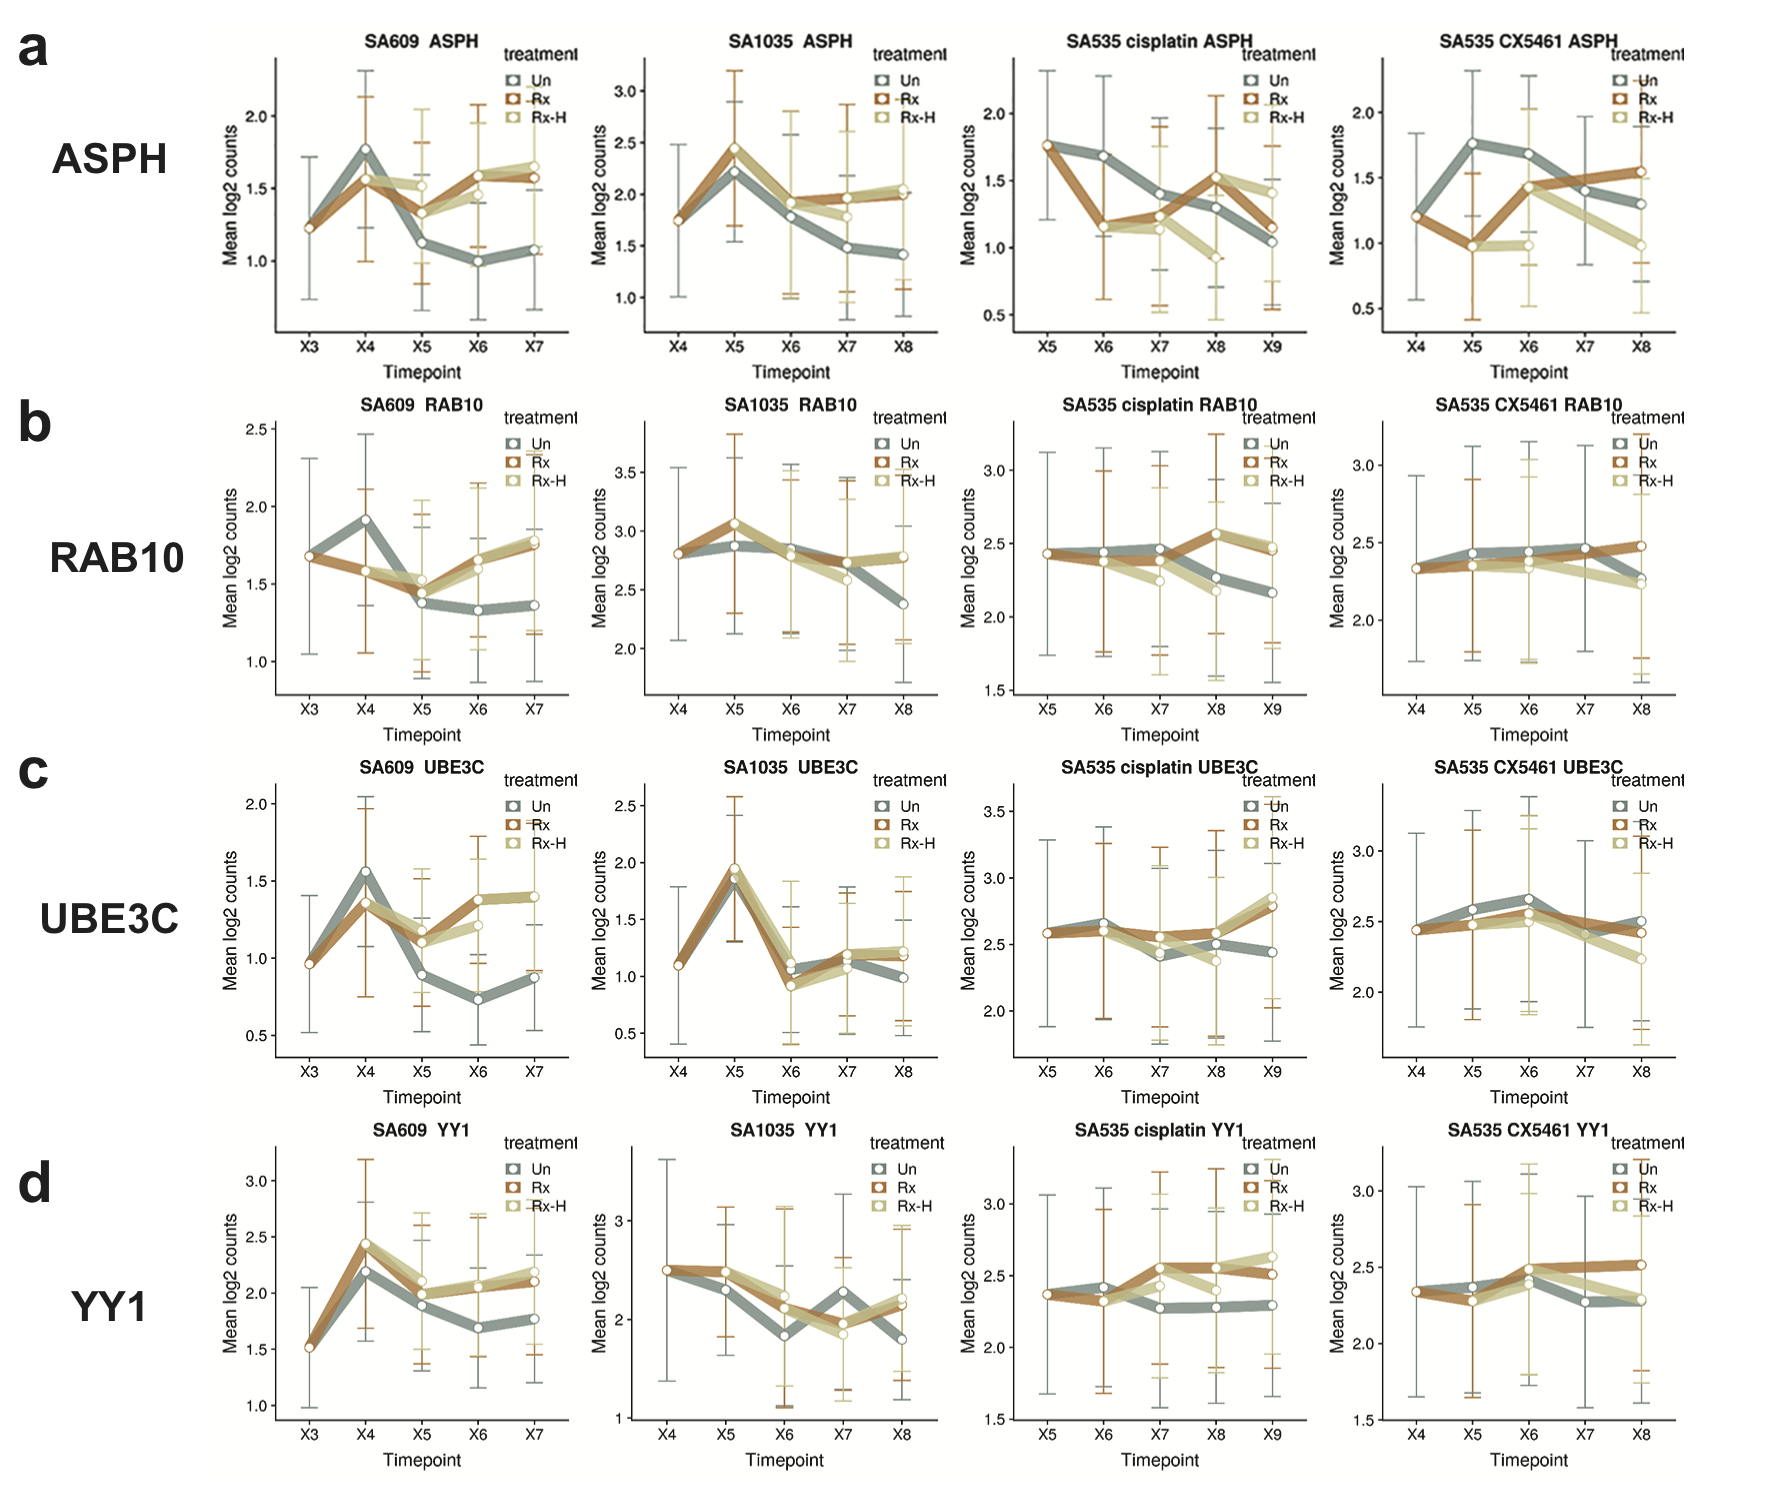
\includegraphics[width=\textwidth]{Figures/chap5/commongenesfromvolcanoplots.png}
	
\caption[Representative trajectories of 4 common genes upregulated in all PDX]
	{\small
	\textbf{Representative trajectories of 4 common genes upregulated in all PDX.}
	   Horizontal axis shows timepoints passages of tumors. First time point is the baseline untreated value and from second timepoint onwards, depicts increasing cycles of chemotherapy or untreated cycles. Vertical axis represents the SCTransform normalized mean log2 counts of gene expression at that time point. Genes upregulated are selected from \ac{DE} of resistant vs sensitive clones and \textbf{\autoref{tab:UpregulatedgenesinalltreatedPDX}}.
	   \textbf{(a)} \textit{ASPH} expression trajectories.
	    \textbf{(b)} \textit{RAB10} expression trajectories.
	    \textbf{(c)} \textit{UBE3C} expression trajectories.
	     \textbf{d)} \textit{YY1} expression trajectories.
	}
	\label{fig:commongenesfromvolcanoplots}
\end{figure}
%----------------------------------------------------------------


CX-5461 treated time dependent expression of \textbf{ID2, TOP2A, MARKCS and PABPC1} are shown in \textbf{\autoref{fig:generegressionanalysis} h}.
\textbf{PABPC1} is known to exert carcinogenesis in gastric carcinoma by targeting miR-34c and it is correlated with tumor progression and has a prognostic role in esophageal cancer \cite{zhu2015pabpc1,takashima2006expression}. \textbf{MARCKS} is known to be over expressed in lung cancers and is known as a novel predictor of cancer malignancy \cite{reddy2014marcks, chen2014novel} \textbf{\autoref{fig:generegressionanalysis} d.}

All these genes found in our timeseries datasets, could act as a potential candidates to be further validated in triple negative breast cancers.

%-------------------------------------------------------------

\section{Discussion}

In this chapter, we began with the intention of identifying the magnitude of expression coupling the change in the copy number defined clonal proportions. By using clonealign, we were able to assign single cell RNAseq to  DLP+ clones and observed similar clonal fractions. \ac{UMAP} suggested that the clones are behaving in relatively monomorphic way. From global survey of the copy number driven change in expression, \textit{in cis} proportion was found to be less as compared to the \textit{in trans} which is consistent with the previous knowledge of mutation effects on expression. We know that cis-regulatory mutations are skewed toward decreased expression while trans-regulatory mutations are skewed toward increased expression \cite{metzger2016contrasting}. Here we show that instead of taking mutation as a marker to identify clones, copy number defined clones could be used to explore expression  space and tumor behaviour at single cell RNAseq level. The importance of studying gene expression along with its regulation 

We also evaluated the expression differences between resistant and sensitive clones across all 4 treated PDX series. We detected a range of two-fold magnitude difference \textit{in cis} and \textit{in trans} on either side of up regulated and down regulated genes. While we observed differences in expression, we sought to elucidate the signaling pathways involved . In breast cancer, so far many molecular pathways have been explicated while many others are either under investigation or to be investigated \cite{hanahan2011hallmarks}. Here, we found the top 5 cisplatin related commonly upregulated pathways in our data sets includes \textbf{TNFA signaling via NF-$\kappa$B, TGF  beta  signaling, apoptosis, hypoxia and estrogen response pathways}. Moreover, \textbf{G2M checkpoint and E2F targets} were also detected highly activated and sharing set of genes in 50\% of our datasets. 

Interestingly, BRCA1 deficient TNBC, SA535 PDX exhibited activation of \textbf{IL-2\_STAT5 signaling} with cisplatin while \textbf{IL-6\_JAK\_STAT5 signaling} was exclusively upregulated with CX-5461 in the same PDX. The potential addition of IL-6/JAK/STAT3 inhibitors with currently approved therapeutic agents directed against immune-checkpoint inhibitors are already under consideration \cite{johnson2018targeting}.

We also summarized common genes, that were found to be upregulated in all of 4 PDX series. Amid this list, we highlighted 4 interesting genes, out of which \textbf{ASPH}, monotonically increased with drug in our datasets, is contracting attention in recent literature as a potential target in cancer therapy \cite{barboro2020aspartate, li2018expression, hou2018recent, kanwal2020aspartate}. Notably, ASPH activates Notch signaling pathway and its upregulated expression stimulates the translocation of Notch to the nucleus consequently governing downstream target genes that mediate breast cancer cell adhesion and metastasis. Furthermore, these malignant phenotypes are reversed using a small molecule inhibitor (MO-I-1182) \cite{lin2019asph}. Aforementioned other genes, \textbf{RAB10}, belongs to the group of Ras-family proto-oncogenes and its knowkdown has been linked to induce cell cycle arrest and apoptosis \cite{zhou2018down}, whereas \textbf{UBE3C and YY1} are known to be uniformly highly over-expressed in a wide range of human cancers and here we nominated them in category of chemotherapy mediated increase in  differential expression in all of our time series \cite{pan2015ubiquitin, zhang2020ube3c, meliala2020biological, wan2012yin}. 

Overall, in single cell expression space, we noticed that SA1035 TNBC PDX behaves a little different as compared to the other two PDX models based on the activated pathways and proportion of individual gene expression \textit{in cis} and \textit{in trans}. This could be possibly explained based on the initial heterogeneity of this tumor from chapter 4. The DLP+ heatmap showed less heterogeneity as compared to SA609 and SA535 that were found to have more complex clonal structures.

 We were able to enumerate common genes that were upregulated in all of our models under chemotherapy exposure, however, most of the other genes were tumor specific explaining the concept of inter tumor heterogeneity.
 




%Next we compared the emerging clone under drug pressure with the clone that could not survive the repeated drug exposures. We identified the following significantly up regulated pathways:
%- Apoptosis, Epithelial mesenchymal transition, Hypoxia, mitotic spindle, MTORC1 signaling, MYC targets-V1, P53 pathway, TGF Beta signaling, TNFA signalling via NF-$\kappa$B, UV response up, UV response down, KRAS signaling, Angiogenesis, PI3K AKT MTOR signaling, unfolded protein response.








